% \documentclass[oneside,final,14pt]{extreport}
% \usepackage{vmargin}
% \setmarginsrb{2cm}{1.5cm}{1cm}{1.5cm}{0pt}{0mm}{0pt}{13mm}
\documentclass[12pt]{article}
% \usepackage[utf8x]{inputenc}
\usepackage[a4paper, total={6in, 8in}]{geometry}
\usepackage{fontspec}
\usepackage{mparhack}
\usepackage{marginnote}
\usepackage{fancyhdr}
\usepackage{hyperref}
\usepackage[stable]{footmisc}
\usepackage{titlesec}
\usepackage{graphicx}

%
% sectioning
%
\titleformat{\paragraph}[hang]{\normalfont\normalsize\bfseries}{\theparagraph}{1em}{}
\titlespacing*{\paragraph}{0pt}{12pt plus 4pt minus 2pt}{0pt plus 2pt minus 2pt}

%
% href setup
%
\hypersetup{
    colorlinks=false, %set true if you want colored links
    linktoc=all,     %set to all if you want both sections and subsections linked
    linkcolor=blue,  %choose some color if you want links to stand out
}

%
% fonts
%
\setmainfont{Arial}
\usepackage[russianb]{babel}

%
% headers/footers
%
\pagestyle{fancy}
% \fancyhead{}
\fancyhf{}

\lhead{\small\rightmark}
\lfoot{\small\leftmark}
\rfoot{\thepage}
% \fancyfoot[CE,CO]{\thepage}
%
% shortcuts
%
\newcommand\ellipsis{%
  \textbackslash\thinspace\textellipsis\textbackslash
}

%
% par spacing
%
\setlength{\parskip}{1em}
\setlength\parindent{0cm}

%
% par numbers
%

\newcommand\resetparcount{%
  \setcounter{parcount}{0}
}

\newcommand{\parnum}{(\arabic{parcount})}

\newcounter{parcount}

\newcommand\p{%
    \stepcounter{parcount}%
    \noindent\marginpar[]{\parnum}%
}

% \newenvironment{parnumbers}{%
%   % \setcounter{parcount}{0}
%    \par%
%    \everypar{\noindent \stepcounter{parcount}\parnum \hspace{1em}}%
% }{}

\newenvironment{parnumbers}{%
  \par%
  \everypar{\noindent \stepcounter{parcount}\marginpar[]{\parnum}}%
}{}

%
% end par numbers
%

%
% misc
%

% remove date from title page
\date{}

\title{%
  Краткий курс марксизма \\
  \large v\input{VERSION}}

\begin{document}

\maketitle

\tableofcontents

\newpage

\section*{Введение}
\label{sec:intro}
% \addtocounter{section}{1}
\markboth{Введение}{Введение}
\addcontentsline{toc}{section}{Введение}


Однажды я вспомнил, что имею диплом преподавателя философии (подходящего к тому же красного цвета), пошел в Ленинскую библиотеку (она для меня всегда останется “Ленинкой”), разыскал там советское методическое пособие по диалектическому и историческому материализму, выкинул из него весь схоластический мусор вроде “Партия и правительство в заботах о советском спорте” и в “сухом остатке” вырисовалась подборка отрывков по 6-ти темам, которые вы найдете ниже.

Как сегодня можно обсуждать классиков марксизма?

Однажды я вспомнил, что имею диплом преподавателя философии (подходящего к тому же красного цвета), пошел в Ленинскую библиотеку (она для меня всегда останется “Ленинкой”), разыскал там советское методическое пособие по диалектическому и историческому материализму, выкинул из него весь схоластический мусор вроде “Партия и правительство в заботах о советском спорте” и в “сухом остатке” вырисовалась подборка отрывков по 6-ти темам, которые вы найдете ниже.

Еще одним методическим принципом стала работа в “малых группах”. Мне с самого начала казалось очень важным уйти от формата “лектор перед аудиторией”, активный “эксперт” и пассивно внимающие ему слушатели. Сегодня ни у кого нет “окончательных” ответов и глупо претендовать на позицию “ментора” - поэтому разговор может быть только равного с равными.

Так что уже несколько лет, когда находится 4-5-6-10 человек, желающих читать и обсуждать эти тексты и способных договориться об общей встрече, мы собираемся с такой группой примерно раз в неделю в разных местах, иногда в профсоюзном офисе, иногда на травке в сквере, но чаще всего в любом кафе, где нет громкой музыки.

Предварительно каждый должен (1) прочитать ту тему, которая будет обсуждаться; и как минимум (2) отметить те места, которые непонятны или вызывают возражения. Так же очень важно, чтобы у каждого (3) был свою экземпляр текста (печатный или электронный). Во-первых, многие вопросы исчезают, если внимательно перечитать непонятый сразу фрагмент (замечал это множество раз). Во-вторых, трех перечисленных условий (прочитать, отметить непонятое, принести текст с пометками с собой) в абсолютном большинстве случаев достаточно, чтобы завязалась оживленная и главное плодотворная дискуссия. (Для того, чтобы быстро найти место, которое предлагается обсудить, все абзацы каждой темы пронумерованы по порядку.)

Поскольку это группа равных, я в качестве модератора в основном слежу за тем, чтобы высказывающиеся не перебивали друг друга и чтобы вопрос, поставленный кем-то, был понятен остальным (иногда для этого его надо повторить или переформулировать).


В малой тесной группе ни у кого практически нет шансов “отсидеться”, отмолчаться. Даже те, кто не любит и не собирается говорить, чаще всего самой энергией общей дискуссии увлекаются и вовлекаются в разговор. Кроме того, естественно, объяснение другим своей точки зрения приводит к лучшему уяснению ее себе самому.


В завершении обсуждения какого-либо фрагмента, перед тем как двинуться дальше или разойтись до следующей встречи, я подвожу итоги и высказываю свое мнение (если оно отлично от уже прозвучавших).


Что касается количества встреч; в принципе одну тему можно обсудить за час-полтора. Но обычно обсуждение длится гораздо дольше. Я никогда не останавливаю его словами типа “достаточно, пора двигаться дальше” (за исключением тех случаев, когда дискуссия очевидно начинает двигаться дважды по одному кругу или из-за признаков усталости присутствующих). Более того, чем больше встреч приходится на одну тему, тем более успешным я считаю обсуждение - значит его участникам было интересно, значит они находили все новые и новые повороты мысли, достйные внимания.


И несколько замечаний напоследок.


1. При первой встрече я всегда оговариваю - цель таких обсуждений не в том, чтобы сделать из участников кружка “истинных марксистов”. Это смешно и просто невозможно даже после подробного обсуждения этих самых базовых, но и самых начальных текстов. Без самостоятельного чтения в дальнейшем гораздо более широкого круга источников (в конце концов марксизм это громадная традиция с почти двухвековой историей, с множеством течений и школ) невозможно подлинное знакомство с “философией практики” и тем более овладение ее методом. Обсуждая эти 6 тем, мы знакомимся лишь с алфавитом марксизма. Для того, чтобы складывать из него слова, а тем более предложения и абзацы - нужно проработать гораздо больше книг. Но и без алфавита этот процесс не начнется.


2. С Марксом можно и нужно спорить. Но прежде чем спорить, нужно понять мысль классиков. Очень часто претензии к ним основаны или на добросовестном заблуждении или на прямом искажении их идей, и спор превращается в то, что в философии называется “логомахия”, когда один спорит о зеленом, а другой о квадратном. Так вот задача наших встреч, как я ее себе понимаю, не столько убедить в непогрешимости классиков, индоктринировать, сколько понять их - а потом уже спорить, соглашаться, развивать, может быть даже отвергать.


3. 90\% этих текстов относятся к 19 веку. Но в процессе обсуждения неизбежно возникают параллели с веком 20-м (особенно с историей СССР) и веком 21-м. Я никогда не обрываю эти уходы в другие времена, но каждый раз подчеркиваю - чтобы судить о таких экстремально сложных вопросах, как история 20 века или история СССР, недостаточно прочитать несколько десятков страниц из Маркса и Ленина. Многое из того, что происходил в 20 веке и происходит в 21-м, было “запрограммировано” в мысли классиков - но далеко не все. На основании текстов 19 века мы можем говорить о последующих событиях и процессах только в самом первом приближении. Если это условие держать в голове, то можно и нужно, конечно, при обсуждении, например, опыта Парижской коммуны говорить об Октябрьской революции или, скажем, о мексиканских сапатистах. И это вполне может стать одним из самых интересных моментов встреч в таком кружке.


4. Неизбежно множество вопросов вызывает “экономический детерминизм” в марксизме. Поэтому после обсуждения всех 6-ти тем, полезно вернтуься к этой проблеме и обсудить главу “Противоречие и сверхдетерминация” из книги Луи Альтюссера “За Маркса”, где ставится под вопрос такой детерминизм - это придает важное “стереоскопическое” измерение данной проблеме.


Не менее жаркие дискуссиии вызывает всегда вопрос определения классов в сегодняшних обществах и вообще классовой структуры общества сегодня. Аналогично, после окончания этого “краткого курса” полезно обсудить статью ведущего исследователя классов в современном мире Эрика Райта “Марксистские концепции классовой структуры”.


И, наконец, особую сложность представляет приложение в первую очередь социально-политико-экономического метода марксизма к такому “тонкому” вопросу и проблеме как искусство. Здесь я бы посоветовал в конце курса отдельно обсудить блестящий образец такого приложения, статью Льва Троцкого “Формальная школа поэзии и марксизм” из книги “Литература и революция”.


Это - лишь 3 варианта продолжения из миллиона других возможных. Они ни в коей мере не являются “завершением” марксистского образования, даже начального, а только расширяют русло, в котором надо двигаться самостоятельно.

Владислав Софронов





\section{Общественное производство}
\resetparcount

\subsection{КАРЛ МАРКС К КРИТИКЕ ПОЛИТИЧЕСКОЙ ЭКОНОМИИ}
\subsubsection*{Предисловие\footnote{Маркс К., Энгельс Ф. Сочинения. - 2-е изд. - Т.13. - С.5-9.}}

\begin{parnumbers}
    Я рассматриваю систему буржуазной экономики в следующем порядке: капитал, земельная собственность, наемный труд, государство, внешняя торговля, мировой рынок. Под первыми тремя рубриками я исследую экономические условия жизни трех больших классов, на которые распадается современное буржуазное общество; взаимная связь трех других рубрик очевидна. Первый отдел первой книги, трактующей о капитале, состоит из следующих глав: 1) товар, 2) деньги, или простое обращение, 3) капитал вообще. Первые две главы составляют содержание настоящего выпуска. Весь материал лежит предо мной в форме монографий, которые были написаны с большими перерывами в различные периоды не для печати, а для уяснения вопросов самому себе; последовательная обработка этих монографий по указанному плану будет зависеть от внешних обстоятельств.

    Общее введение, которое я было набросал, я опускаю, так как по более основательном размышлении решил, что всякое предвосхищение выводов, которые еще только должны быть доказаны, может помешать, а читатель, который вообще захочет следовать за мной, должен решиться восходить от частного к общему. Однако некоторые замечания о ходе моих собственных политико-экономических занятий представляются мне здесь уместными.

    Моим специальным предметом была юриспруденция, которую, однако, я изучал лишь как подчиненную дисциплину наряду с философией и историей. В 1842-1843 гг. мне как редактору "Rheinische Zeitung" пришлось впервые высказываться о так называемых материальных интересах, и это поставило меня в затруднительное положение. Обсуждение в рейнском ландтаге вопросов о краже леса и дроблении земельной собственности, официальная полемика, в которую г-н фон Шaпер, тогдашний обер- президент Рейнской провинции, вступил с "Rheinische Zeitung" относительно положения мозельских крестьян, наконец, дебаты о свободе торговли и покровительственных пошлинах дали первые толчки моим занятиям экономическими вопросами. С другой стороны, в это время, когда благое желание "идти вперед" во много раз превышало знание предмета, в "Rheinische Zeitung" послышались отзвуки французского социализма и коммунизма со слабой философской окраской. Я высказался против этого дилетантства, но вместе с тем в полемике с аугсбургской "Allgemeine Zeitung" откровенно признался, что мои тогдашние знания не позволяли мне отважиться на какое-либо суждение о самом содержании французских направлений. Тем с большей охотой я воспользовался иллюзией руководителей "Rheinische Zeitung", которые надеялись более умеренной позицией добиться отмены вынесенного ей смертного приговора, чтобы удалиться с общественной арены в учебную комнату.

    Первая работа, которую я предпринял для разрешения обуревавших меня сомнений, был критический разбор гегелевской философии права; введение к этой работе появилось в 1844 г. в издававшемся в Париже "Deutsch-Franzosische Jahrbucher". Мои исследования привели меня к тому результату, что правовые отношения, так же точно как и формы государства, не могут быть поняты ни из самих себя, ни из так называемого общего развития человеческого духа, что, наоборот, они коренятся в материальных жизненных отношениях, совокупность которых Гегель, по примеру английских и французских писателей XVIII века, называет "гражданским обществом", и что анатомию гражданского общества следует искать в политической экономии. Начатое мною в Париже изучение этой последней я продолжал в Брюсселе, куда я переселился вследствие приказа г-на Гизо о моей высылке из Парижа. Общий результат, к которому я пришел и который послужил затем руководящей нитью в моих дальнейших исследованиях, может быть кратко сформулирован следующим образом. В общественном производстве своей жизни люди вступают в определенные, необходимые, от их воли не зависящие отношения - производственные отношения, которые соответствуют определенной ступени развития их материальных производительных сил. Совокупность этих производственных отношений составляет экономическую структуру общества, реальный базис, на котором возвышается юридическая и политическая надстройка и которому соответствуют определенные формы общественного сознания. Способ производства материальной жизни обусловливает социальный, политический и духовный процессы жизни вообще. Не сознание людей определяет их бытие, а, наоборот, их общественное бытие определяет их сознание. На известной ступени своего развития материальные производительные силы общества приходят в противоречие с существующими производственными отношениями, или - что является только юридическим выражением последних - с отношениями собственности, внутри которых они до сих пор развивались. Из форм развития производительных сил эти отношения превращаются в их оковы. Тогда наступает эпоха социальной революции. С изменением экономической основы более или менее быстро происходит переворот во всей громадной надстройке. При рассмотрении таких переворотов необходимо всегда отличать материальный, с естественно-научной точностью констатируемый переворот в экономических условиях производства от юридических, политических, религиозных, художественных или философских, короче - от идеологических форм, в которых люди осознают этот конфликт и борются за его разрешение. Как об отдельном человеке нельзя судить на основании того, что сам он о себе думает, точно так же нельзя судить о подобной эпохе переворота по ее сознанию. Наоборот, это сознание надо объяснить из противоречий материальной жизни, из существующего конфликта между общественными производительными силами и производственными отношениями. Ни одна общественная формация не погибает раньше, чем разовьются все производительные силы, для которых она дает достаточно простора, и новые более высокие производственные отношения никогда не появляются раньше, чем созреют материальные условия их существования в недрах самого старого общества. Поэтому человечество ставит себе всегда только такие задачи, которые оно может разрешить, так как при ближайшем рассмотрении всегда оказывается, что сама задача возникает лишь тогда, когда материальные условия ее решения уже имеются налицо, или, по крайней мере, находятся в процессе становления. В общих чертах, азиатский, античный, феодальный и современный, буржуазный, способы производства можно обозначить как прогрессивные эпохи экономической общественной формации. Буржуазные производственные отношения являются последней антагонистической формой общественного процесса производства, антагонистической не в смысле индивидуального антагонизма, а в смысле антагонизма, вырастающего из общественных условий жизни индивидуумов; но развивающиеся в недрах буржуазного общества производительные силы создают вместе с тем материальные условия для разрешения этого антагонизма. Поэтому буржуазной общественной формацией завершается предыстория человеческого общества.

    Фридрих Энгельс, с которым я со времени появления его гениальных набросков к критике экономических категорий (в "Deutsch-Franzosische Jahrbucher") поддерживал постоянный письменный обмен мнениями, пришел другим путем к тому же результату, что и я (ср. его "Положение рабочего класса в Англии"; и когда весной 1845 г. он также поселился в Брюсселе, мы решили сообща разработать наши взгляды в противоположность идеологическим взглядам немецкой философии, в сущности свести счеты с нашей прежней философской совестью. Это намерение было осуществлено в форме критики послегегелевской философии. Рукопись - в объеме двух толстых томов в восьмую долю листа - давно ужо прибыла на место издания в Вестфалию, когда нас известили, что изменившиеся обстоятельства делают ее напечатание невозможным. Мы тем охотнее предоставили рукопись грызущей критике мышей, что наша главная цель - уяснение дела самим себе - была достигнута. Из отдельных работ, в которых мы в то время с той или иной стороны изложили наши взгляды публике, я упомяну лишь написанный совместно Энгельсом и мной "Манифест Коммунистической партии" и опубликованную мной "Речь о свободе торговли". Решающие пункты наших воззрений были впервые научно изложены, хотя только в полемической форме, в моей работе "Нищета философии", выпущенной в 1847 г. и направленной против Прудона. Февральская революция и последовавшее в связи с ней насильственное удаление меня из Бельгии прервали печатание написанной на немецком языке работы о "Наемном труде", в которой я собрал лекции, читанные мною в Немецком рабочем обществе в Брюсселе. Издание "Neue Rheinische Zeitung" в 1848 и 1849 гг. и последовавшие затем события прервали мои экономические занятия, которые я смог возобновить только в 1850 г. в Лондоне. Огромный материал по истории политической экономии, собранный в Британском музее, то обстоятельство, что Лондон представляет собой удобный наблюдательный пункт для изучения буржуазного общества, наконец, новая стадия развития, в которую последнее, казалось, вступило с открытием калифорнийского и австралийского золота, - все это побудило меня приняться за изучение предмета с начала и критически переработать новый материал. Эти занятия приводили, отчасти сами собой, к вопросам на первый взгляд совершенно не относящимся к предмету, но на которых я должен был останавливаться более или менее продолжительное время. Но особенно сокращалось имевшееся в моем распоряжении время вследствие настоятельной необходимости работать ради хлеба насущного. Мое теперь уже восьмилетнее сотрудничество в "New-York Daily Tribune", первой англо-американской газете (собственно газетные корреспонденции я пишу только в виде исключения), делало необходимым чрезвычайно частые перерывы в моих научных занятиях. Однако статьи о выдающихся экономических событиях в Англии и на континенте составляли настолько значительную часть моей работы для газеты, что я принужден был познакомиться с практическими деталями, лежащими за пределами собственно науки политической экономии.

    Эти заметки о ходе моих занятий в области политической экономии должны лишь показать, что мои взгляды, как бы о них ни судили и как бы мало они ни согласовались с эгоистическими предрассудками господствующих классов, составляют результат добросовестных и долголетних исследований. А у входа в науку, как и у входа в ад, должно быть выставлено требование: "Qui si convien lasciare ogni sospetto; Ogni viltа convien che qui sia morta"*. (— «Здесь нужно, чтоб душа была тверда; Здесь страх не должен подавать совета» (Данте. «Божественная комедия»).
\end{parnumbers}

\subsection{ФРИДРИХ ЭНГЕЛЬС \\
«АНТИ-ДЮРИНГ». ОТДЕЛ III: СОЦИАЛИЗМ}
\subsubsection*{ГЛ. II. ОЧЕРК ТЕОРИИ}

\begin{parnumbers}
    Материалистическое понимание истории исходит из того положения, что производство, а вслед за производством обмен его продуктов, составляет основу всякого общественного строя; что в каждом выступающем в истории обществе распределение продуктов, а вместе с ним и разделение общества на классы или сословия, определяется тем, что и как производится, и как эти продукты производства обмениваются. Таким образом, конечных причин всех общественных изменений и политических переворотов надо искать не в головах людей, не в возрастающем понимании ими вечной истины и справедливости, а в изменениях способа производства и обмена; их надо искать не в философии, а в экономике соответствующей эпохи. Пробуждающееся понимание того, что существующие общественные установления неразумны и несправедливы, что «разумное стало бессмысленным, благо стало мучением», —является лишь симптомом того, что в методах производства и в формах обмена незаметно произошли такие изменения, которым уже не соответствует общественный строй, скроенный по старым экономическим условиям. Отсюда вытекает также и то, что средства для устранения обнаруженных зол должны быть тоже налицо — в более или менее развитом виде — в самих изменившихся производственных отношениях. Надо не изобретать эти средства из головы, а открывать их при помощи головы в наличных материальных фактах производства.

    Итак, как же, в связи с этим, обстоит дело с современным социализмом? Всеми уже, пожалуй, признано, что существующий общественный строй создан господствующим теперь классом — буржуазией. Свойственный буржуазии способ производства, называемый со времени Маркса капиталистическим способом производства, был несовместим с местными и сословными привилегиями, равно как и с взаимными личными узами феодального строя; буржуазия разрушила феодальный строй и воздвигла на его развалинах буржуазный общественный строй, царство свободной конкуренции, свободы передвижения, равноправия товаровладельцев, — словом, всех буржуазных прелестей. Капиталистический способ производства мог теперь развиваться свободно. C тех пор как пар и новые рабочие машины превратили старую мануфактуру в крупную промышленность, созданные под управлением буржуазии производительные силы стали развиваться с неслыханной прежде быстротой и в небывалых размерах.

    Но точно так же, как в свое время мануфактура и усовершенствовавшиеся под ее
    влиянием ремесла пришли в конфликт с феодальными оковами цехов, так и крупная промышленность в своем более полном развитии приходит в конфликт с теми узкими рамками, в которые ее втискивает капиталистический способ производства. Новые производительные силы уже переросли буржуазную форму их использования. И этот конфликт между производительными силами и способом производства вовсе не такой конфликт, который возник только в головах людей — подобно конфликту между человеческим первородным грехом и божественной справедливостью, — а существует в действительности, объективно, вне нас, независимо от воли или поведения даже тех людей, деятельностью которых он создан. Современный социализм есть не что иное, как отражение в мышлении этого фактического конфликта, идеальное отражение его в головах прежде всего того класса, который страдает от него непосредственно, — рабочего класса.

    В чем же состоит этот конфликт? До появления капиталистического производства, т. е. в средние века, всюду существовало мелкое производство, основой которого была частная собственность работников на их средства производства: в деревне — земледелие мелких крестьян, свободных или крепостных, в городе — ремесло. Средства труда — земля, земледельческие орудия, мастерские, ремесленные инструменты — были средствами труда отдельных лиц, рассчитанными лишь на единоличное употребление, и, следовательно, по необходимости оставались мелкими, карликовыми, ограниченными. Но потому-то они, как правило, и принадлежали самому производителю. Сконцентрировать, укрупнить эти раздробленные, мелкие средства производства, превратить их в современные могучие рычаги производства — такова как раз и была историческая роль капиталистического способа производства и его носительницы — буржуазии. Как она исторически выполнила эту роль, начиная с XV века, на трех различных ступенях производства: простой кооперации, мануфактуры и крупной промышленности, — подробно изображено Марксом в IV отделе «Капитала». Но буржуазия, как установил Маркс там же, не могла превратить эти ограниченные средства производства в мощные производительные силы, не превращая их из средств производства, применяемых отдельными лицами, в общественные. средства производства, применяемые лишь совместно массой людей. Вместо самопрялки, ручного ткацкого станка, кузнечного молота появились прядильная машина, механический ткацкий станок, паровой молот; вместо отдельной мастерской — фабрика, требующая совместного труда сотен и тысяч рабочих. Подобно средствам производства, и само производство превратилось из ряда разрозненных действий в ряд общественных действий, а продукты — из продуктов отдельных лиц в продукты общественные. Пряжа, ткани, металлические товары, выходящие теперь из фабрик и заводов, представляют собой продукт совместного труда множества рабочих, через руки которых они должны были последовательно пройти, прежде чем стали готовыми. Никто в отдельности не может сказать о них: «Это сделал я, это мой продукт».

    Но там, где основной формой производства является стихийно сложившееся разделение труда в обществе, там это разделение труда неизбежно придает продуктам форму товаров, взаимный обмен которых, купля и продажа, дает возможность отдельным производителям удовлетворять свои разнообразные потребности. Так и было в средние века. Крестьянин, например, продавал ремесленнику земледельческие продукты и покупал у него ремесленные изделия. В это общество отдельных производителей, товаропроизводителей, и вклинился новый способ производства. Среди стихийно сложившегося, беспланового разделения труда, господствующего во всем обществе, он установил планомерное разделение труда, организованное на каждой отдельной фабрике; рядом с производством отдельных производителей появилось общественное производство. Продукты того и другого продавались на одном и том же рынке, а следовательно, по ценам, по крайней мере, приблизительно одинаковым. Но планомерная организация оказалась могущественнее стихийно сложившегося разделения труда; на фабриках, применявших общественный труд, изготовление продуктов обходилось дешевле, чем у разрозненных мелких производителей. Производство отдельных производителей побивалось в одной области за другой, общественное производство революционизировало весь старый способ производства.

    Однако этот революционный характер общественного производства так мало сознавался, что оно, напротив, вводилось именно ради усиления и расширения товарного производства. Оно возникло в непосредственной связи с определенными, уже до него существовавшими рычагами производства и обмена товаров: купеческим капиталом, ремеслом и наемным трудом.

    Ввиду того что оно само выступало как новая форма товарного производства, свойственные товарному производству формы присвоения сохраняли свою полную силу также и для него.

    При той форме товарного производства, которая развивалась в средние века, вопрос о том, кому должен принадлежать продукт труда, не мог даже и возникнуть. Он изготовлялся от- дельным производителем обыкновенно из собственного сырья, часто им же самим произве- денного, при помощи собственных средств труда и собственными руками или руками семьи.

    Такому производителю незачем было присваивать себе этот продукт, он принадлежал ему по самому существу дела. Следовательно, право собственности на продукты покоилось на собственном труде. Даже там, где пользовались посторонней помощью, она, как правило, играла лишь побочную роль и зачастую вознаграждалась помимо заработной платы еще и иным путем: цеховой ученик и подмастерье работали не столько ради содержания и платы, сколько ради собственного обучения и подготовки к званию самостоятельного мастера. Но вот началась концентрация средств производства в больших мастерских и мануфактурах, превращение их по сути дела в общественные средства производства. С этими общественными средствами производства и продуктами продолжали, однако, поступать так, как будто они по-прежнему оставались средствами производства и продуктами отдельных лиц. Если до сих пор собственник средств труда присваивал продукт потому, что это был, как правило, его собственный продукт, а чужой вспомогательный труд был исключением, то теперь собственник средств труда продолжал присваивать себе продукт, хотя последний являлся уже не его продуктом, а исключительно продуктом чужого труда. Таким образом, продукты общественного труда стали присваиваться не теми, кто действительно приводил в движение средства производства и действительно был производителем этих продуктов, а капиталистом.

    Средства производства и производство по существу стали общественными. Но они остаются подчиненными той форме присвоения, которая своей предпосылкой имеет частное производство отдельных производителей, когда каждый, следовательно, является владельцем своего продукта и выносит его на рынок. Способ производства подчиняется этой форме присвоения, несмотря на то, что он уничтожает ее предпосылку. (Нет надобности разъяснять здесь, что если форма присвоения и остается прежней, то характер присвоения претерпевает вследствие вышеописанного процесса не меньшую революцию, чем характер производства.

    Присваиваю ли я продукт своего собственного или продукт чужого труда — это, конечно, два весьма различных вида присвоения. Заметим мимоходом, что наемный труд, в котором уже содержится в зародыше весь капиталистический способ производства, существует с давних времен; в единичной, случайной форме он существовал в течение столетий рядом с рабством. Но этот зародыш мог развиться в капиталистический способ производства только тогда, когда были созданы необходимые для этого исторические предпосылки.) В этом противоречии, которое придает новому способу производства его капиталистический характер, уже содержатся в зародыше все коллизии современности. И чем полнее становилось господство нового способа производства во всех решающих отраслях производства и во всех экономически господствующих странах, сводя тем самым производство отдельных производителей к незначительным остаткам, тем резче должна была выступать и несовместимость общественного производства с капиталистическим присвоением.

    Первые капиталисты застали, как мы видели, форму наемного труда уже существующей. Но наемный труд существовал лишь в виде исключения, побочного занятия, подсобного промысла, переходного положения. Земледелец, нанимавшийся время от времени на поденную работу, имел свой собственный клочок земли, который на худой конец и один мог его прокормить. Цеховые уставы заботились о том, чтобы сегодняшний подмастерье завтра становился мастером. Но все изменилось, как только средства производства превратились в общественные и сконцентрировались в руках капиталистов. Средства производства и продукты мелкого отдельного производителя все более и более обесценивались, и ему не оставалось ничего иного, как наниматься к капиталисту. Наемный труд, существовавший раньше в виде исключения и подсобного промысла, стал правилом и основной формой всего производства; из побочного занятия, каким он был прежде, он превратился теперь в единственную деятельность работника. Работник, нанимающийся время от времени, превратился в пожизненного наемного рабочего. Масса пожизненных наемных рабочих к тому же чрезвычайно увеличилась благодаря одновременному крушению феодального строя, роспуску свит феодалов, изгнанию крестьян из их усадеб и т. д. Произошел полный разрыв между средствами производства, сконцентрированными в руках капиталистов, с одной стороны, и производителями, лишенными всего, кроме своей рабочей силы, с другой стороны. Противоречие между общественным производством и капиталистическим присвоением выступает наружу как антагонизм между пролетариатом и буржуазией.

    Мы видели, что капиталистический способ производства вклинился в общество, состояв- шее из товаропроизводителей, отдельных производителей, общественная связь между кото- рыми осуществлялась посредством обмена их продуктов. Но особенность каждого общества, основанного на товарном производстве, заключается в том, что в нем производители теряют власть над своими собственными общественными отношениями. Каждый производит сам по себе, случайно имеющимися у него средствами производства и для своей индивидуальной потребности в обмене. Никто не знает, сколько появится на рынке того продукта, который он производит, и в каком количестве этот продукт вообще может найти потребителей; никто не знает, существует ли действительная потребность в производимом им продукте, окупятся ли его издержки производства, да и вообще будет ли его продукт продан. В общественном производстве господствует анархия. Но товарное производство, как и всякая другая форма производства, имеет свои особые, внутренне присущие ему и неотделимые от него законы; и эти законы прокладывают себе путь вопреки анархии, в самой этой анархии, через нее. Эти законы проявляются в единственно сохранившейся форме общественной связи — в обмене — и действуют на отдельных производителей как принудительные законы конкуренции. Они, следовательно, сначала неизвестны даже самим производителям и могут быть открыты ими лишь постепенно, путем долгого опыта. Следовательно, они прокладывают себе путь помимо производителей и против производителей, как слепо действующие естественные законы их формы производства. Продукт господствует над производителями.

    В средневековом обществе, в особенности в первые столетия, производство было направлено, главным образом, на собственное потребление. Оно удовлетворяло по преимуществу только потребности самого производителя и его семьи. Там же, где, как в деревне, существовали отношения личной зависимости, производство удовлетворяло также потребности феодала. Следовательно, здесь не существовало никакого обмена, и продукты не принимали характера товаров. Крестьянская семья производила почти все, в чем она нуждалась: орудия и одежду, так же как и предметы питания. Производить на продажу она начала только тогда, когда стала производить излишек сверх собственного потребления и уплаты натуральных повинностей феодалу; этот излишек, пущенный в общественный обмен, предназначенный для продажи, становился товаром. Городские ремесленники должны были, конечно, уже с самого начала производить для обмена. Но и они добывали большую часть нужных для собственного потребления предметов своим личным трудом: они имели огороды и небольшие поля, пасли свой скот в общинном лесу, который, кроме того, доставлял им строительный материал и топливо; женщины пряли лен, шерсть и т. д. Производство с целью обмена, товарное производство еще только возникало. Отсюда — ограниченность обмена, ограниченность рынка, стабильность способа производства, местная замкнутость по отношению к внешнему миру, местное объединение внутри: марка в деревне, цех в городе.

    С расширением же товарного производства и в особенности с появлением капиталистического способа производства дремавшие раньше законы товарного производства стали действовать более открыто и властно. Старые связи были расшатаны, былые перегородки разрушены, и производители все более и более превращались в независимых, разрозненных товаропроизводителей. Анархия общественного производства выступила наружу и принимала все более и более острый характер. А между тем главное орудие, с помощью которого капиталистический способ производства усиливал анархию в общественном производстве, представляло собой прямую противоположность анархии: это была растущая организация производства как производства общественного на каждом отдельном производственном предприятии. С помощью этого рычага капиталистический способ производства покончил со старой мирной стабильностью. Проникая в ту или иную отрасль промышленности, он изгонял из нее старые методы производства. Овладевая ремеслом, он уничтожал старое ремесло. Поле труда стало полем битвы. Великие географические открытия и последовавшая за ними колонизация увеличили во много раз область сбыта и ускорили превращение ремесла в мануфактуру. Борьба разгоралась уже не только между местными отдельными производителями; местные схватки разрослись, в свою очередь, до размеров борьбы между нациями, до торговых войн XVII и XVIII веков. Наконец, крупная промышленность и возникновение мирового рынка сделали эту борьбу всеобщей и в то же время придали ей неслыханную ожесточенность. В отношениях между отдельными капиталистами, как и между целыми отраслями производства и между целыми странами, вопрос о существовании решается тем, обладают ли они выгодными, естественными или искусственно созданными, условиями производства.

    Побежденные безжалостно устраняются. Это — дарвиновская борьба за отдельное существование, перенесенная — с удесятеренной яростью — из природы в общество. Естественное состояние животных выступает как венец человеческого развития. Противоречие между общественным производством и капиталистическим присвоением воспроизводится как противоположность между организацией производства на отдельных фабриках и анархией производства во всем обществе.

    В этих обеих формах проявления противоречия, присущего капиталистическому способу производства в силу его происхождения, безвыходно движется этот способ производства, описывая «порочный круг», который открыл в нем уже Фурье. Но Фурье в свое время еще не мог, конечно, видеть, что этот круг постепенно суживается, что движение производства идет скорее по спирали и, подобно движению планет, должно закончиться столкновением с центром. Движущая сила общественной анархии производства все более и более превращает большинство человечества в пролетариев, а пролетарские массы, в свою очередь, уничтожат в конце концов анархию производства. Та же движущая сила социальной анархии производства превращает возможность бесконечного усовершенствования машин, применяемых в крупной промышленности, в принудительный закон для каждого отдельного промышленного капиталиста, в закон, повелевающий ему беспрерывно совершенствовать свои машины под страхом гибели. Но усовершенствование машин делает излишним определенное количество человеческого труда. Если введение и распространение машин означало вытеснение миллионов работников ручного труда немногими рабочими при машинах, то усовершенствование машин означает вытеснение все большего и большего количества самих рабочих машинного труда и, в конечном счете, образование усиленного предложения рабочих рук, превышающего средний спрос на них со стороны капитала. Масса незанятых рабочих образует настоящую промышленную резервную армию, как я назвал ее еще в 1845 г.*, поступающую в распоряжение производства, когда оно работает на всех парах, и выбрасываемую на мостовую в результате неизбежно следующего за этим краха; эта армия, постоянно висящая свинцовой гирей на ногах рабочего класса в борьбе за существование между ним и капиталом, служит регулятором заработной платы, удерживая ее на низком уровне, соответственно потребности капитала. Таким образом, выходит, что машина, говоря словами Маркса, становится самым мощным боевым средством капитала против рабочего класса, что средство труда постоянно вырывает из рук рабочего жизненные средства и собственный продукт рабочего превращается в орудие его порабощения. Это приводит к тому, что экономия на средствах труда с самого начала является, вместе с тем, беспощаднейшим расточением рабочей силы и хищничеством по отношению к нормальным условиям функционирования труда; что машина, это сильнейшее средство сокращения рабочего времени, превращается в самое верное средство для того, чтобы обратить всю жизнь рабочего и его семьи в потенциальное рабочее время для увеличения стоимости капитала.

    Вот почему чрезмерный труд одной части рабочего класса обусловливает полную безработицу другой его части, а крупная промышленность, по всему свету гоняющаяся за потребителями, ограничивает у себя дома потребление рабочих масс голодным минимумом и таким образом подрывает свой собственный внутренний рынок. «Закон, поддерживающий относительное перенаселение, или промышленную резервную армию, в равновесии с размерами и энергией накопления капитала, приковывает рабочего к капиталу крепче, чем молот Гефеста приковал Прометея к скале. Он обусловливает накопление нищеты, соответственное накоплению капитала. Следовательно, накопление богатства на одном полюсе есть в то же время накопление нищеты, муки труда, рабства, невежества, огрубения и моральной деградации на противоположном полюсе, т. е. на стороне класса, который производит свой собственный продукт как капитал» (Маркс, «Капитал», стр. 671). Ждать от капиталистического способа производства иного распределения продуктов имело бы такой же смысл, как требовать, чтобы электроды батареи, оставаясь соединенными с ней, перестали разлагать воду и собирать на положительном полюсе кислород, а на отрицательном — водород.

    Мы видели, как способность современных машин к усовершенствованию, доведенная до высочайшей степени, превращается, вследствие анархии производства в обществе, в принудительный закон, заставляющий отдельных промышленных капиталистов постоянно улучшать свои машины, постоянно увеличивать их производительную силу. В такой же принудительный закон превращается для них и простая фактическая возможность расширять размеры своего производства. Огромная способность крупной промышленности к расширению, перед которой расширяемость газов оказывается настоящей детской забавой, проявляется теперь в виде потребности расширять эту промышленность и качественно, и количественно, — потребности, не считающейся ни с каким противодействием. Это противодействие образуется потреблением, сбытом, рынками для продуктов крупной промышленности. Способность же рынков как к экстенсивному, так и к интенсивному расширению определяется совсем иными законами, действующими с гораздо меньшей энергией. Расширение рынков не может поспевать за расширением производства. Коллизия становится неизбежной, и так как она не в состоянии разрешить конфликт до тех пор, пока не взорвет самый капиталистический способ производства, то она становится периодической. Капиталистическое производство порождает новый «порочный круг».

    И действительно, начиная с 1825 г., когда разразился первый общий кризис, весь промышленный и торговый мир, производство и обмен всех цивилизованных народов вместе с их более или менее варварскими придатками приблизительно раз в десять лет сходят с рельсов. В торговле наступает застой, рынки переполняются массой не находящих сбыта продуктов, наличные деньги исчезают из обращения, кредит прекращается, фабрики останавливаются, рабочие лишаются жизненных средств, ибо они произвели эти средства в слишком большом количестве; банкротства следуют за банкротствами, аукционы сменяются аукционами. Застой длится годами, массы производительных сил и продуктов расточаются и уничтожаются, пока накопившиеся массы товаров по более или менее сниженным ценам не разойдутся, наконец, и не возобновится постепенно движение производства и обмена. Мало-помалу движение это ускоряется, шаг сменяется рысью, промышленная рысь переходит в галоп, уступающий свое место бешеному карьеру, настоящей скачке с препятствиями, охватывающей промышленность, торговлю, кредит и спекуляцию, чтобы в конце концов после самых отчаянных скачков снова свалиться в бездну краха. И так постоянно сызнова. С 1825 г. мы уже пять раз пережили этот круговорот и теперь (в 1877 г.) переживаем его в шестой раз. Характер этих кризисов выражен до такой степени ярко, что Фурье уловил суть всех этих кризисов, назвав первый из них crise plethorique, кризисом от изобилия.

    В кризисах с неудержимой силой прорывается наружу противоречие между общественным производством и капиталистическим присвоением. Обращение товаров на время прекращается; средство обращения — деньги — становится тормозом обращения; все законы производства и обращения товаров действуют навыворот. Экономическая коллизия достигает своей высшей точки: способ производства восстает против способа обмена, производительные силы восстают против способа производства, который они переросли.

    Тот факт, что общественная организация производства внутри фабрик достигла такой степени развития, что стала несовместимой с существующей рядом с ней и над ней анархией производства в обществе, — этот факт становится осязательным для самих капиталистов благодаря насильственной концентрации капиталов, совершающейся во время кризисов посредством разорения многих крупных и еще большего числа мелких капиталистов. Весь механизм капиталистического способа производства отказывается служить под тяжестью им же самим созданных производительных сил. Он не может уже превращать в капитал всю массу средств производства; они остаются без употребления, а потому вынуждена бездействовать и промышленная резервная армия. Средства производства, жизненные средства, рабочие, находящиеся в распоряжении капитала, — все элементы производства и общего благосостояния имеются в изобилии. Но «изобилие становится источником нужды и лишений» (Фурье), потому что именно оно-то и препятствует превращению средств производства и жизненных средств в капитал. Ибо в капиталистическом обществе средства производства не могут вступать в действие иначе, как превратившись сначала в капитал, в средство эксплуатации человеческой рабочей силы. Как призрак, стоит между рабочими, с одной стороны, и средствами производства и жизненными средствами, с другой, необходимость превращения этих средств в капитал. Она одна препятствует соединению вещественных и личных рычагов производства; она одна мешает средствам производства действовать, а рабочим — трудиться и жить. Следовательно, с одной стороны, капиталистический способ производства изобличается в своей собственной неспособности к дальнейшему управлению производительными силами. С другой стороны, сами производительные силы с возрастающей мощью стремятся к уничтожению этого противоречия, к освобождению себя от всего того, что свойственно им в качестве капитала, к фактическому признанию их характера как общественных производительных сил.

    Это противодействие мощно возрастающих производительных сил их капиталистическому характеру, эта возрастающая необходимость признания их общественной природы принуждает класс самих капиталистов все чаще и чаще обращаться с ними, насколько это вообще возможно при капиталистических отношениях, как с общественными производительными силами. Как периоды промышленной горячки с их безгранично раздутым кредитом, так и самые крахи, разрушающие крупные капиталистические предприятия, приводят к такой форме обобществления больших масс средств производства, какую мы встречаем в различного рода акционерных обществах. Некоторые из этих средств производства и сообщения, как, например, железные дороги, сами по себе до того колоссальны, что они исключают всякую другую форму капиталистической эксплуатации. На известной ступени развития становится недостаточной и эта форма: государство как официальный представитель капиталистического общества вынуждено взять на себя руководство указанными средствами производства и сообщения. Эта необходимость превращения в государственную собственность наступает прежде всего для крупных средств сообщения: почты, телеграфа и железных дорог.

    Если кризисы выявили неспособность буржуазии к дальнейшему управлению современными производительными силами, то переход крупных производственных предприятий и средств сообщения в руки акционерных обществ и в государственную собственность доказывает ненужность буржуазии для этой цели. Все общественные функции капиталиста выполняются теперь наемными служащими. Для капиталиста не осталось другой общественной деятельности, кроме загребания доходов, стрижки купонов и игры на бирже, где различные капиталисты отнимают друг у друга капиталы. Если раньше капиталистический способ производства вытеснял рабочих, то теперь он вытесняет и капиталистов, правда, пока еще не в промышленную резервную армию, а только в разряд излишнего населения.

    Но ни переход в руки акционерных обществ, ни превращение в государственную собственность не уничтожают капиталистического характера производительных сил. Относительно акционерных обществ это совершенно очевидно. А современное государство опять-таки есть лишь организация, которую создает себе буржуазное общество для охраны общих внешних условий капиталистического способа производства от посягательств как рабочих, так и отдельных капиталистов. Современное государство, какова бы ни была его форма, есть по самой своей сути капиталистическая машина, государство капиталистов, идеальный совокупный капиталист. Чем больше производительных сил возьмет оно в свою собственность, тем полнее будет его превращение в совокупного капиталиста и тем большее число граждан будет оно эксплуатировать. Рабочие останутся наемными рабочими, пролетариями. Капиталистические отношения не уничтожаются, а, наоборот, доводятся до крайности, до высшей точки. Но на высшей точке происходит переворот. Государственная собственность на производительные силы не разрешает конфликта, но она содержит в себе формальное средство, возможность его разрешения.

    Это разрешение может состоять лишь в том, что общественная природа современных производительных сил будет признана на деле и что, следовательно, способ производства, присвоения и обмена будет приведен в соответствие с общественным характером средств производства. А это может произойти только таким путем, что общество открыто и не прибегая ни к каким окольным путям возьмет в свое владение производительные силы, переросшие всякий другой способ управления ими, кроме общественного. Тем самым общественный характер средств производства и продуктов, который теперь оборачивается против самих производителей и периодически потрясает способ производства и обмена, прокладывая себе путь только как слепо действующий закон природы, насильственно и разрушительно, — этот общественный характер будет тогда использован производителями с полной сознательностью и превратится из причины расстройств и периодических крахов в сильнейший рычаг самого производства.

    Общественные силы, подобно силам природы, действуют слепо, насильственно, разрушительно, пока мы не познали их и не считаемся с ними. Но раз мы познали их, поняли их действие, направление и влияние, то только от нас самих зависит подчинять их все более и более нашей воле и с их помощью достигать наших целей. Это в особенности относится к современным могучим производительным силам. Пока мы упорно отказываемся понимать их природу и характер, — а этому пониманию противятся капиталистический способ производства и его защитники, — до тех пор производительные силы действуют вопреки нам, против нас, до тех пор они властвуют над нами, как это подробно показано выше. Но раз понята их природа, они могут превратиться в руках ассоциированных производителей из демонических повелителей в покорных слуг. Здесь та же разница, что между разрушительной силой электричества в грозовой молнии и укрощенным электричеством в телеграфном аппарате и дуговой лампе, та же разница, что между пожаром и огнем, действующим на службе человека.

    Когда с современными производительными силами станут обращаться сообразно с их познанной, наконец, природой, общественная анархия в производстве заменится общественно-планомерным регулированием производства сообразно потребностям как общества в целом, так и каждого его члена в отдельности. Тогда капиталистический способ присвоения, при котором продукт порабощает сперва производителя, а затем и присвоителя, будет заменен новым способом присвоения продуктов, основанным на самой природе современных средств производства: с одной стороны, прямым общественным присвоением продуктов в качестве средств для поддержания и расширения производства, а с другой — прямым индивидуальным присвоением их в качестве средств к жизни и наслаждению.

    Все более и более превращая громадное большинство населения в пролетариев, капиталистический способ производства создает силу, которая под угрозой гибели вынуждена совершить этот переворот. Заставляя все более и более превращать в государственную собственность крупные обобществленные средства производства, капиталистический способ производства сам указывает путь к совершению этого переворота. Пролетариат берет государственную власть и превращает средства производства прежде всего в государственную собственность. Но тем самым он уничтожает самого себя как пролетариат, тем самым он уничтожает все классовые различия и классовые противоположности, а вместе с тем и государство как государство. Существовавшему и существующему до сих пор обществу, которое движется в классовых противоположностях, было необходимо государство, т. е. организация эксплуататорского класса для поддержания его внешних условий производства, значит, в особенности для насильственного удержания эксплуатируемого класса в определяемых данным способом производства условиях подавления (рабство, крепостничество или феодальная зависимость, наемный труд). Государство было официальным представителем всего общества, его сосредоточением в видимой корпорации, но оно было таковым лишь постольку, поскольку оно было государством того класса, который для своей эпохи один представлял все общество: в древности оно было государством рабовладельцев — граждан государства, в средние века — феодального дворянства, в наше время — буржуазии. Когда государство наконец-то становится действительно представителем всего общества, тогда оно само себя делает излишним. С того времени, когда не будет ни одного общественного класса, который надо бы было держать в подавлении, с того времени, когда исчезнут вместе с классовым господством, вместе с борьбой за отдельное существование, порождаемой теперешней анархией в производстве, те столкновения и эксцессы, которые проистекают из этой борьбы, — с этого времени нечего будет подавлять, не будет и надобности в особой силе для подавления, в государстве. Первый акт, в котором государство выступает действительно как представитель всего общества — взятие во владение средств производства от имени общества, — является в то же время последним самостоятельным актом его как государства. Вмешательство государственной власти в общественные отношения становится тогда в одной области за другой излишним и само собой засыпает. На место управления лицами становится управление вещами и руководство производственными процессами. Государство не «отменяется», оно отмирает. На основании этого следует оценивать фразу про «свободное народное государство», фразу, имевшую до известной поры право на существование в качестве агитационного средства, но в конечном счете научно несостоятельную. На основании этого следует оценивать также требование так называемых анархистов, чтобы государство было отменено с сегодня на завтра.

    С тех пор как на историческую сцену выступил капиталистический способ производства, взятие обществом всех средств производства в свое владение часто представлялось в виде более или менее туманного идеала будущего как отдельным личностям, так и целым сектам.

    Но оно стало возможным, стало исторической необходимостью лишь тогда, когда материальные условия его проведения в жизнь оказались налицо. Как и всякий другой общественный прогресс, оно становится осуществимым не вследствие осознания того, что существование классов противоречит справедливости, равенству и т. д., не вследствие простого желания отменить классы, а в силу известных новых экономических условий. Разделение общества на классы — эксплуатирующий и эксплуатируемый, господствующий и угнетенный — было неизбежным следствием прежнего незначительного развития производства. Пока совокупный общественный труд дает продукцию, едва превышающую самые необходимые средства существования всех, пока, следовательно, труд отнимает все или почти все время огромного большинства членов общества, до тех пор это общество неизбежно делится на классы. Рядом с этим огромным большинством, исключительно занятым подневольным трудом, образуется класс, освобожденный от непосредственно производительного труда и ведающий такими общими делами общества, как управление трудом, государственные дела, правосудие, науки, искусства и т. д. Следовательно, в основе деления на классы лежит закон разделения труда. Это, однако, отнюдь не исключало применения насилия, хищничества, хитрости и обмана при образовании классов и не мешало господствующему классу, захватившему власть, упрочивать свое положение за счет трудящихся классов и превращать руководство обществом в эксплуатацию масс.

    Но если разделение на классы имеет, таким образом, известное историческое оправдание, то оно имеет его лишь для известного периода и при известных общественных условиях. Оно обусловливалось недостаточностью производства и будет уничтожено полным развитием современных производительных сил. И действительно, упразднение общественных классов предполагает достижение такой ступени исторического развития, на которой является анахронизмом, выступает как отжившее не только существование того или другого определенного господствующего класса, но и какого бы то ни было господствующего класса Вообще, а следовательно, и самое деление на классы. Следовательно, упразднение классов предполагает такую высокую ступень развития производства, на которой присвоение особым общественным классом средств производства и продуктов, — а с ними и политического господства, монополии образования и духовного руководства, — не только становится излишним, но и является препятствием для экономического, политического и интеллектуального развития. Эта ступень теперь достигнута. Политическое и интеллектуальное банкротство буржуазии едва ли составляет тайну даже для нее самой, а ее экономическое банкротство повторяется регулярно каждые десять лет. При каждом кризисе общество задыхается под тяжестью своих собственных производительных сил и продуктов, которые оно не может использовать, и остается беспомощным перед абсурдным противоречием, когда производители не могут потреблять потому, что недостает потребителей. Свойственная современным средствам производства сила расширения разрывает оковы, наложенные капиталистическим способом производства. Освобождение средств производства от этих оков есть единственное предварительное условие беспрерывного, постоянно ускоряющегося развития производительных сил, а благодаря этому — и практически безграничного роста самого производства.

    Но этого недостаточно. Обращение средств производства в общественную собственность устраняет не только существующее теперь искусственное торможение производства, но также и то прямое расточение и уничтожение производительных сил и продуктов, которое в на-стоящее время является неизбежным спутником производства и достигает своих высших размеров в кризисах. Сверх того, оно сберегает для общества массу средств производства и продуктов путем устранения безумной роскоши и мотовства господствующих теперь классов и их политических представителей. Возможность обеспечить всем членам общества путем общественного производства не только вполне достаточные и с каждым днем улучшающиеся материальные условия существования, но также полное свободное развитие и применение их физических и духовных способностей, — эта возможность достигнута теперь впервые, но теперь она действительно достигнута.

    Раз общество возьмет во владение средства производства, то будет устранено товарное производство, а вместе с тем и господство продукта над производителями. Анархия внутри общественного производства заменяется планомерной, сознательной организацией. Прекращается борьба за отдельное существование. Тем самым человек теперь — в известном смысле окончательно — выделяется из царства животных и из звериных условий существования переходит в условия действительно человеческие. Условия жизни, окружающие людей и до сих пор над ними господствовавшие, теперь подпадают под власть и контроль людей, которые впервые становятся действительными и сознательными повелителями природы, потому что они становятся господами своего собственного объединения в общество. Законы их собственных общественных действий, противостоявшие людям до сих пор как чуждые, господствующие над ними законы природы, будут применяться людьми с полным знанием дела и тем самым будут подчинены их господству. То объединение людей в общество, которое противостояло им до сих пор как навязанное свыше природой и историей, становится теперь их собственным свободным делом.

    Объективные, чуждые силы, господствовавшие до сих пор над историей, поступают под контроль самих людей. И только с этого момента люди начнут вполне сознательно сами творить свою историю, только тогда приводимые ими в движение общественные причины будут иметь в преобладающей и все возрастающей мере и те следствия, которых они желают. Это есть скачок человечества из царства необходимости в царство свободы. Совершить этот освобождающий мир подвиг — таково историческое призвание современного пролетариата. Исследовать исторические условия, а вместе с тем и самоё природу этого переворота и таким образом выяснить ныне угнетенному классу, призванному совершить этот подвиг, условия и природу его собственного дела — такова задача научного социализма, являющегося теоретическим выражением пролетарского движения.
\end{parnumbers}

\subsection{Ф. ЭНГЕЛЬС \\
    ПИСЬМО В. БОРГИУСУ, 25 ЯНВАРЯ 1894 г.}

\begin{parnumbers}
  Лондон, 25 января 1894 г. \\
    Милостивый государь! \\
    Отвечаю на Ваши вопросы: \\
    1. Под экономическими отношениями, которые мы считаем определяющим базисом истории общества, мы понимаем тот способ, каким люди определенного общества производят средства к жизни и обменивают между собой продукты (поскольку существует разделение труда). Таким образом, сюда входит вся техника производства и транспорта. Эта техника, согласно нашим взглядам, определяет также и способ обмена, затем способ распределения продуктов и тем самым после разложения родового строя также и разделение на классы, отношения господства и подчинения, государство, политику, право и т. д. В понятие экономических отношений включается далее и географическая основа, на которой эти отношения развиваются, и фактически перешедшие от прошлого остатки прежних ступеней экономического развития, которые продолжают сохраняться зачастую только по традиции или благодаря vis inertiae (силе инерции), а также, конечно, внешняя среда, окружающая эту общественную форму.

    Если, как Вы утверждаете, техника в значительной степени зависит от состояния науки, то в гораздо большей мере наука зависит от состояния и потребностей техники. Если у общества появляется техническая потребность, то это продвигает науку вперед больше, чем десяток университетов. Вся гидростатика (Торричелли и т. д.) была вызвана к жизни потребностью регулировать горные потоки в Италии в XVI и XVII веках. Об электричестве мы узнали кое-что разумное только с тех пор, как была открыта его техническая применимость. В Германии, к сожалению, привыкли писать историю наук так, как будто бы науки свалились с неба.

    2. Мы считаем, что экономические условия в конечном счете обусловливают историческое развитие. Раса же сама является экономическим фактором. Здесь, однако, не следует забывать о двух моментах:

    а) Политическое, правовое, философское, религиозное, литературное, художественное и т. д. развитие основано на экономическом развитии. Но все они также оказывают влияние друг на друга и на экономический базис. Дело обстоит совсем не так, что только экономическое положение является причиной, что только оно является активным, а все остальное — лишь пассивное следствие. Нет, тут взаимодействие на основе экономической необходимости, в конечном счете всегда прокладывающей себе путь. Государство, например, оказывает влияние при помощи покровительственных пошлин, свободы торговли, хорошей или дурной фискальной политики. Даже смертельная усталость и бессилие немецкого мещанина, обусловленные жалким экономическим положением Германии в период с 1648 по 1830 г. и выразившиеся сначала в пиетизме, затем в сентиментальсти или рабском пресмыкательстве перед князьями и дворянством, не остались без влияния на экономику. Это было одним из величайших препятствий для нового подъема, и препятствие это было поколеблено только благодаря тому, что революционные и наполеоновские войны сделали хроническую нищету острой. Следовательно, экономическое положение не оказывает своего воздействия автоматически, как это для удобства кое-кто себе представляет, а люди сами делают свою историю, однако в данной, их обусловливающей среде, на основе уже существующих действительных отношений, среди которых экономические условия, как бы сильно ни влияли на них прочие — политические и идеологические, — являются в конечном счете все же решающими и образуют ту красную нить, которая пронизывает все развитие и одна приводит к его пониманию.

    в) Люди сами делают свою историю, но до сих пор они делали ее, не руководствуясь общей волей, по единому общему плану, и даже не в рамках определенным образом ограниченного, данного общества. Их стремления перекрещиваются, и во всех таких обществах господствует поэтому необходимость, дополнением и формой проявления которой является случайность. Необходимость, пробивающаяся здесь сквозь все случайности, — опять-таки в конечном счете экономическая. Здесь мы подходим к вопросу о так называемых великих людях. То обстоятельство, что такой и именно вот этот великий человек появляется в определенное время в данной стране, конечно, есть чистая случайность. Но если этого человека устранить, то появляется спрос на его замену, и такая замена находится — более или менее, удачная, но с течением времени находится. Что Наполеон, именно этот корсиканец, был тем военным диктатором, который стал необходим Французской республике, истощенной войной, — это было случайностью. Но если бы Наполеона не было, то роль его выполнил бы другой. Это доказывается тем, что всегда, когда такой человек был нужен, он находился: Цезарь, Август, Кромвель и т. д. Если материалистическое понимание истории открыл Маркс, то Тьерри, Минье, Гизо, все английские историки до 1850 г. служат доказательством того, что дело шло к этому, а открытие того же самого понимания Морганом показывает, что время для этого созрело и это открытие должно было быть сделано.

    Точно так же обстоит дело со всеми другими случайностями и кажущимися случайностями в истории. Чем дальше удаляется от экономической та область, которую мы исследуем, чем больше она приближается к чисто абстрактно-идеологической, тем больше будем мы находить в ее развитии случайностей, тем более зигзагообразной является ее кривая. Если Вы начертите среднюю ось кривой, то найдете, что чем длиннее изучаемый период, чем шире изучаемая область, тем более приближается эта ось к оси экономического развития, тем более параллельно ей она идет.

    В Германии величайшим препятствием к правильному пониманию является непростительное пренебрежение в литературе к экономической истории. Не только очень трудно отвыкнуть от представлений об историческом развитии, привитых в школе, но еще труднее собрать материал, необходимый для этого. Кто читал, например, хотя бы старого Г. фон Гюлиха, который в своем сухом собрании материалов поместил столько ценного для объяснения бесчисленного множества политических фактов!

    Вообще же я думаю, что тот прекрасный образец, который Маркс дал в «Восемнадцатом брюмера», должен дать Вам довольно полный ответ на Ваши вопросы как раз потому, что это — практический пример. Большинство вопросов, как мне кажется, затронуто в «Анти- Дюринге», отдел первый, гл. IX— XI, отдел второй, гл. II—IV, отдел третий, гл. I или во введении, а кроме того, и в последней главе «Фейербаха» (Ф. Энгельс. «Людвиг Фейербах и конец классической немецкой философии»).

    Прошу Вас не относиться придирчиво к каждому слову из вышеизложенного, а все время иметь в виду общую связь; у меня, к сожалению, не было времени изложить Вам все так ясно и четко, как следовало бы, если бы это предназначалось для печати.
\end{parnumbers}




\section{Классы и классовая борьба}
\resetparcount
\subsection{К.МАРКС и Ф.ЭНГЕЛЬС.  МАНИФЕСТ КОММУНИСТИЧЕСКОЙ ПАРТИИ \footnote{ПСС, 2-е изд. Т. 4.}}
\subsubsection*{БУРЖУА И ПРОЛЕТАРИИ\footnote{Под буржуазией понимается класс современных капиталистов, собственников средств общественного производства, применяющих наемный труд. Под пролетариатом понимается класс современных наемных рабочих, которые, будучи лишены своих собственных средств производства, вынуждены, для того чтобы жить, продавать свою рабочую силу. (Примечание Энгельса к английскому изданию 1888 г.}}
\begin{parnumbers}
    История всех до сих пор существовавших обществ была историей борьбы классов. Свободный и раб, патриций и плебей, помещик и крепостной, мастер и подмастерье, короче, угнетающий и угнетаемый находились в вечном антагонизме друг к другу, вели непрерывную, то скрытую, то явную борьбу, всегда кончавшуюся революционным переустройством всего общественного здания или общей гибелью борющихся классов. В предшествующие исторические эпохи мы находим почти повсюду полное расчленение общества на различные сословия,- целую лестницу различных общественных положений. В Древнем Риме мы встречаем патрициев, всадников, плебеев, рабов; в средние века - феодальных господ, вассалов, цеховых мастеров, подмастерьев, крепостных, и к тому же почти в каждом из этих классов - еще особые градации.

    Вышедшее из недр погибшего феодального общества современное буржуазное общество не уничтожило классовых противоречий. Оно только поставило новые классы, новые условия угнетения и новые формы борьбы на место старых. Наша эпоха, эпоха буржуазии, отличается, однако, тем, что она упростила классовые противоречия: общество все более и более раскалывается на два большие враждебные лагеря, на два большие, стоящие друг против друга, класса - буржуазию и пролетариат.

    Из крепостных средневековья вышло свободное население первых городов; из этого сословия горожан развились первые элементы буржуазии.

    Открытие Америки и морского пути вокруг Африки создало для подымающейся буржуазии новое поле деятельности. Ост-индский и китайский рынки, колонизация Америки, обмен с колониями, увеличение количества средств обмена и товаров вообще дали неслыханный до тех пор толчок торговле, мореплаванию, промышленности и тем самым вызвали в распадавшемся феодальном обществе быстрое развитие революционного элемента.

    Прежняя феодальная, или цеховая, организация промышленности более не могла удовлетворить спроса, возраставшего вместе с новыми рынками. Место ее заняла мануфактура. Цеховые мастера были вытеснены промышленным средним сословием; разделение труда между различными корпорациями исчезло, уступив место разделению труда внутри отдельной мастерской. Но рынки все росли, спрос все увеличивался. Удовлетворить его не могла уже и мануфактура. Тогда пар и машина произвели революцию в промышленности. Место мануфактуры заняла современная крупная промышленность, место промышленного среднего сословия заняли миллионеры-промышленники, предводители целых промышленных армий, современные буржуа.

    Крупная промышленность создала всемирный рынок, подготовленный открытием Америки. Всемирный рынок вызвал колоссальное развитие торговли, мореплавания и средств сухопутного сообщения. Это в свою очередь оказало воздействие на расширение промышленности, и в той же мере, в какой росли промышленность, торговля, мореплавание, железные дороги, развивалась буржуазия, она увеличивала свои капиталы и оттесняла на задний план все классы, унаследованные от средневековья. Мы видим, таким образом, что современная буржуазия сама является продуктом длительного процесса развития, ряда переворотов в способе производства и обмена.

    Каждая из этих ступеней развития буржуазии сопровождалась соответствующим политическим успехом. Угнетенное сословие при господстве феодалов, вооруженная и самоуправляющаяся ассоциация в коммуне, тут - независимая городская республика, там - третье, податное сословие монархии, затем, в период мануфактуры, - противовес дворянству в сословной или в абсолютной монархии и главная основа крупных монархий вообще, наконец, со времени установления крупной промышленности и всемирного рынка, она завоевала себе исключительное политическое господство в современном представительном государстве. Современная государственная власть - это только комитет, управляющий общими делами всего класса буржуазии. Буржуазия сыграла в истории чрезвычайно революционную роль. Буржуазия, повсюду, где она достигла господства, разрушила все феодальные, патриархальные, идиллические отношения. Безжалостно разорвала она пестрые феодальные путы, привязывавшие человека к его "естественным повелителям", и не оставила между людьми никакой другой связи, кроме голого интереса, бессердечного "чистогана". В ледяной воде эгоистического расчета потопила она священный трепет религиозного экстаза, рыцарского энтузиазма, мещанской сентиментальности. Она превратила личное достоинство человека в меновую стоимость и поставила на место бесчисленных пожалованных и благоприобретенных свобод одну бессовестную свободу торговли. Словом, эксплуатацию, прикрытую религиозными и политическими иллюзиями, она заменила эксплуатацией открытой, бесстыдной, прямой, черствой.

    Буржуазия лишила священного ореола все роды деятельности, которые до тех пор считались почетными и на которые смотрели с благоговейным трепетом. Врача, юриста, священника, поэта, человека науки она превратила в своих платных наемных работников.

    Буржуазия сорвала с семейных отношений их трогательно сентиментальный покров и свела их к чисто денежным отношениям.

    Буржуазия показала, что грубое проявление силы в средние века, вызывающее такое восхищение у реакционеров, находило себе естественное дополнение в лени и неподвижности. Она впервые показала, чего может достигнуть человеческая деятельность. Она создала чудеса искусства, но совсем иного рода, чем египетские пирамиды, римские водопроводы и готические соборы; она совершила совсем иные походы, чем переселение народов и крестовые походы. Буржуазия не может существовать, не вызывая постоянно переворотов в орудиях производства, не революционизируя, следовательно, производственных отношений, а стало быть, и всей совокупности общественных отношений. Напротив, первым условием существования всех прежних промышленных классов было сохранение старого способа производства в неизменном виде. Беспрестанные перевороты в производстве, непрерывное потрясение всех общественных отношений, вечная неуверенность и движение отличают буржуазную эпоху от всех других. Все застывшие, покрывшиеся ржавчиной отношения, вместе с сопутствующими им, веками освященными представлениями и воззрениями, разрушаются, все возникающие вновь оказываются устарелыми, прежде чем успевают окостенеть. Все сословное и застойное исчезает, все священное оскверняется, и люди приходят, наконец, к необходимости взглянуть трезвыми глазами на свое жизненное положение и свои взаимные отношения.

    Потребность в постоянно увеличивающемся сбыте продуктов гонит буржуазию по всему земному шару. Всюду должна она внедриться, всюду обосноваться, всюду установить связи.

    Буржуазия путем эксплуатации всемирного рынка сделала производство и потребление всех стран космополитическим. К великому огорчению реакционеров она вырвала из-под ног промышленности национальную почву. Исконные национальные отрасли промышленности уничтожены и продолжают уничтожаться с каждым днем. Их вытесняют новые отрасли промышленности, введение которых становится вопросом жизни для всех цивилизованных наций, - отрасли, перерабатывающие уже не местное сырье, а сырье, привозимое из самых отдаленных областей земного шара, и вырабатывающие фабричные продукты, потребляемые не только внутри данной страны, но и во всех частях света. Вместо старых потребностей, удовлетворявшихся отечественными продуктами, возникают новые, для удовлетворения которых требуются продукты самых отдаленных стран и самых различных климатов. На смену старой местной и национальной замкнутости и существованию за счет продуктов собственного производства приходит всесторонняя связь и всесторонняя зависимость наций друг от друга. Это в равной мере относится как к материальному, так и к духовному производству. Плоды духовной деятельности отдельных наций становятся общим достоянием. Национальная односторонность и ограниченность становятся все более и более невозможными, и из множества национальных и местных литератур образуется одна всемирная литература.

    Буржуазия быстрым усовершенствованием всех орудий производства и бесконечным облегчением средств сообщения вовлекает в цивилизацию все, даже самые варварские, нации. Дешевые цены ее товаров - вот та тяжелая артиллерия, с помощью которой она разрушает все китайские стены и принуждает к капитуляции самую упорную ненависть варваров к иностранцам. Под страхом гибели заставляет она все нации принять буржуазный способ производства, заставляет их вводить у себя так называемую цивилизацию, т. е. становиться буржуа. Словом, она создает себе мир по своему образу и подобию.

    Буржуазия подчинила деревню господству города. Она создала огромные города, в высокой степени увеличила численность городского населения по сравнению с сельским и вырвала таким образом значительную часть населения из идиотизма деревенской жизни. Так же как деревню она сделала зависимой от города, так варварские и полуварварские страны она поставила в зависимость от стран цивилизованных, крестьянские народы - от буржуазных народов, Восток – от Запада.

    Буржуазия все более и более уничтожает раздробленность средств производства, собственности и населения. Она сгустила население, централизовала средства производства, концентрировала собственность в руках немногих. Необходимым следствием этого была политическая централизация. Независимые, связанные почти только союзными отношениями области с различными интересами, законами, правительствами и таможенными пошлинами, оказались сплоченными в одну нацию, с одним правительством, с одним законодательством, с одним национальным классовым интересом, с одной таможенной границей.

    Буржуазия менее чем за сто лет своего классового господства создала более многочисленные и более грандиозные производительные силы, чем все предшествовавшие поколения, вместе взятые. Покорение сил природы, машинное производство, применение химии в промышленности и земледелии, пароходство, железные дороги, электрический телеграф, освоение для земледелия целых частей света, приспособление рек для судоходства, целые, словно вызванные из-под земли, массы населения, - какое из прежних столетий могло подозревать, что такие производительные силы дремлют в недрах общественного труда!

    Итак, мы видели, что средства производства и обмена, на основе которых сложилась буржуазия, были созданы в феодальном обществе. На известной ступени развития этих средств производства и обмена отношения, в которых происходили производство и обмен феодального общества, феодальная организация земледелия и промышленности, одним словом, феодальные отношения собственности, уже перестали соответствовать развившимся производительным силам. Они тормозили производство, вместо того чтобы его развивать. Они превратились в его оковы. Их необходимо было разбить, и они были разбиты.

    Место их заняла свободная конкуренция, с соответствующим ей общественным и политическим строем, с экономическим и политическим господством класса буржуазии.

    Подобное же движение совершается на наших глазах. Современное буржуазное общество, с его буржуазными отношениями производства и обмена, буржуазными отношениями собственности, создавшее как бы по волшебству столь могущественные средства производства и обмена, походит на волшебника, который не в состоянии более справиться с подземными силами, вызванными его заклинаниями. Вот уже несколько десятилетий история промышленности и торговли представляет собой лишь историю возмущения современных производительных сил против современных производственных отношений, против тех отношений собственности, которые являются условием существования буржуазии и ее господства. Достаточно указать на торговые кризисы, которые, возвращаясь периодически, все более и более грозно ставят под вопрос существование всего буржуазного общества. Во время торговых кризисов каждый раз уничтожается значительная часть не только изготовленных продуктов, но даже созданных уже производительных сил. Во время кризисов разражается общественная эпидемия, которая всем предшествующим эпохам показалась бы нелепостью, - эпидемия перепроизводства. Общество оказывается вдруг отброшенным назад к состоянию внезапно наступившего варварства, как будто голод, всеобщая опустошительная война лишили его всех жизненных средств; кажется, что промышленность, торговля уничтожены, - и почему? Потому, что общество обладает слишком большой цивилизацией, имеет слишком много жизненных средств, располагает слишком большой промышленностью и торговлей.

    Производительные силы, находящиеся в его распоряжении, не служат более развитию буржуазных отношений собственности; напротив, они стали непомерно велики для этих отношений, буржуазные отношения задерживают их развитие; и когда производительные силы начинают преодолевать эти преграды, они приводят в расстройство все буржуазное общество, ставят под угрозу существование буржуазной собственности. Буржуазные отношения стали слишком узкими, чтобы вместить созданное ими богатство. - Каким путем преодолевает буржуазия кризисы?

    С одной стороны, путем вынужденного уничтожения целой массы производительных сил, с другой стороны, путем завоевания новых рынков и более основательной эксплуатации старых. Чем же, следовательно? Тем, что она подготовляет более всесторонние и более сокрушительные кризисы и уменьшает средства противодействия им.

    Оружие, которым буржуазия ниспровергла феодализм, направляется теперь против самой буржуазии.

    Но буржуазия не только выковала оружие, несущее ей смерть; она породила и людей, которые направят против нее это оружие, - современных рабочих, пролетариев.

    В той же самой степени, в какой развивается буржуазия, т. е. капитал, развивается и пролетариат, класс современных рабочих, которые только тогда и могут существовать, когда находят работу, а находят ее лишь до тех пор, пока их труд увеличивает капитал. Эти рабочие, вынужденные продавать себя поштучно, представляют собой такой же товар, как и всякий другой предмет торговли, а потому в равной мере подвержены всем случайностям конкуренции, всем колебаниям рынка.

    Вследствие возрастающего применения машин и разделения труда, труд пролетариев утратил всякий самостоятельный характер, а вместе с тем и всякую привлекательность для рабочего. Рабочий становится простым придатком машины, от него требуются только самые простые, самые однообразные, легче всего усваиваемые приемы. Издержки на рабочего сводятся поэтому почти исключительно к жизненным средствам, необходимым для его содержания и продолжения его рода. Но цена всякого товара, а следовательно и труда, равна издержкам его производства. Поэтому в той же самой мере, в какой растет непривлекательность труда, уменьшается заработная плата. Больше того: в той же мере, в какой возрастает применение машин и разделение труда, возрастает и количество труда, за счет ли увеличения числа рабочих часов, или же вследствие увеличения количества труда, требуемого в каждый данный промежуток времени, ускорения хода машин и т. д.

    Современная промышленность превратила маленькую мастерскую патриархального мастера в крупную фабрику промышленного капиталиста. Массы рабочих, скученные на фабрике, организуются по-солдатски. Как рядовые промышленной армии, они ставятся под надзор целой иерархии унтер-офицеров и офицеров. Они - рабы не только класса буржуазии, буржуазного государства, ежедневно и ежечасно порабощает их машина, надсмотрщик и прежде всего сам отдельный буржуа-фабрикант. Эта деспотия тем мелочнее, ненавистнее, она тем больше ожесточает, чем откровеннее ее целью провозглашается нажива.

    Чем менее искусства и силы требует ручной труд, т. е. чем более развивается современная промышленность, тем более мужской труд вытесняется женским и детским. По отношению к рабочему классу различия пола и возраста утрачивают всякое общественное значение. Существуют лишь рабочие инструменты, требующие различных издержек в зависимости от возраста и пола.

    Когда заканчивается эксплуатация рабочего фабрикантом и рабочий получает, наконец, наличными свою заработную плату, на него набрасываются другие части буржуазии - домовладелец, лавочник, ростовщик и т. п.

    Низшие слои среднего сословия: мелкие промышленники, мелкие торговцы и рантье, ремесленники и крестьяне - все эти классы опускаются в ряды пролетариата, частью оттого, что их маленького капитала недостаточно для ведения крупных промышленных предприятий и он не выдерживает конкуренции с более крупными капиталистами, частью потому, что их профессиональное мастерство обесценивается в результате введения новых методов производства. Так рекрутируется пролетариат из всех классов населения,

    Пролетариат проходит различные ступени развития. Его борьба против буржуазии начинается вместе с его существованием. Сначала борьбу ведут отдельные рабочие, потом рабочие одной фабрики, затем рабочие одной отрасли труда в одной местности против отдельного буржуа, который их непосредственно эксплуатирует. Рабочие направляют свои удары не только против буржуазных производственных отношений, но и против самих орудий производства; они уничтожают конкурирующие иностранные товары, разбивают машины, поджигают фабрики, силой пытаются восстановить потерянное положение средневекового рабочего.

    На этой ступени рабочие образуют рассеянную по всей стране и раздробленную конкуренцией массу. Сплочение рабочих масс пока является еще не следствием их собственного объединения, а лишь следствием объединения буржуазии, которая для достижения своих собственных политических целей должна, и пока еще может, приводить в движение весь пролетариат. На этой ступени пролетарии борются, следовательно, не со своими врагами, а с врагами своих врагов - с остатками абсолютной монархии, землевладельцами, непромышленными буржуа, мелкими буржуа.

    Все историческое движение сосредоточивается, таким образом, в руках буржуазии; каждая одержанная в таких условиях победа является победой буржуазии. Но с развитием промышленности пролетариат не только возрастает численно; он скопляется в большие массы, сила его растет, и он все более ее ощущает.

    Интересы и условия жизни пролетариата все более и более уравниваются по мере того, как машины все более стирают различия между отдельными видами труда и почти всюду низводят заработную плату до одинаково низкого уровня. Возрастающая конкуренция буржуа между собою и вызываемые ею торговые кризисы ведут к тому, что заработная плата рабочих становится все неустойчивее; все быстрее развивающееся, непрерывное совершенствование машин делает жизненное положение пролетариев все менее обеспеченным; столкновения между отдельным рабочим и отдельным буржуа все более принимают характер столкновений между двумя классами. Рабочие начинают с того, что образуют коалиции против буржуа; они выступают сообща для защиты своей заработной платы. Они основывают даже постоянные ассоциации для того, чтобы обеспечить себя средствами на случай возможных столкновений. Местами борьба переходит в открытые восстания.

    Рабочие время от времени побеждают, но эти победы лишь преходящи. Действительным результатом их борьбы является не непосредственный успех, а все шире распространяющееся объединение рабочих. Ему способствуют все растущие средства сообщения, создаваемые крупной промышленностью и устанавливающие связь между рабочими различных местностей. Лишь эта связь и требуется для того, чтобы централизовать многие местные очаги борьбы, носящей повсюду одинаковый характер, и слить их в одну национальную, классовую борьбу. А всякая классовая борьба есть борьба политическая. И объединение, для которого средневековым горожанам с их проселочными дорогами требовались столетия, достигается современными пролетариями, благодаря железным дорогам, в течение немногих лет.

    Эта организация пролетариев в класс, и тем самым - в политическую партию, ежеминутно вновь разрушается конкуренцией между самими рабочими. Но она возникает снова и снова, становясь каждый раз сильнее, крепче, могущественнее.

    Она заставляет признать отдельные интересы рабочих в законодательном порядке, используя для этого раздоры между отдельными слоями буржуазии. Например, закон о десятичасовом рабочем дне в Англии.

    Вообще столкновения внутри старого общества во многих отношениях способствуют процессу развития пролетариата. Буржуазия ведет непрерывную борьбу: сначала против аристократии, позднее против тех частей самой же буржуазии, интересы которых приходят в противоречие с прогрессом промышленности, и постоянно - против буржуазии всех зарубежных стран. Во всех этих битвах она вынуждена обращаться к пролетариату, призывать его на помощь и вовлекать его таким образом в политическое движение. Она, следовательно, сама передает пролетариату элементы своего собственного образования, т. е. оружие против самой себя.

    Далее, как мы видели, прогресс промышленности сталкивает в ряды пролетариата целые слои господствующего класса или, по крайней мере, ставит под угрозу условия их жизни. Они также приносят пролетариату большое количество элементов образования. Наконец, в те периоды, когда классовая борьба приближается к развязке, процесс разложения внутри господствующего класса, внутри всего старого общества принимает такой бурный, такой резкий характер, что небольшая часть господствующего класса отрекается от него и примыкает к революционному классу, к тому классу, которому принадлежит будущее. Вот почему, как прежде часть дворянства переходила к буржуазии, так теперь часть буржуазии переходит к пролетариату, именно - часть буржуа-идеологов, которые возвысились до теоретического понимания всего хода исторического движения.

    Из всех классов, которые противостоят теперь буржуазии, только пролетариат представляет собой действительно революционный класс. Все прочие классы приходят в упадок и уничтожаются с развитием крупной промышленности, пролетариат же есть ее собственный продукт.

    Средние сословия: мелкий промышленник, мелкий торговец, ремесленник и крестьянин - все они борются с буржуазией для того, чтобы спасти свое существование от гибели, как средних сословий. Они, следовательно, не революционны, а консервативны. Даже более, они реакционны: они стремятся повернуть назад колесо истории. Если они революционны, то постольку, поскольку им предстоит переход в ряды пролетариата, поскольку они защищают не свои настоящие, а свои будущие интересы, поскольку они покидают свою собственную точку зрения для того, чтобы встать на точку зрения пролетариата. Люмпен-пролетариат, этот пассивный продукт гниения самых низших слоев старого общества, местами вовлекается пролетарской революцией в движение, но в силу всего своего жизненного положения он гораздо более склонен продавать себя для реакционных козней.

    Жизненные условия старого общества уже уничтожены в жизненных условиях пролетариата. У пролетария нет собственности; его отношение к жене и детям не имеет более ничего общего с буржуазными семейными отношениями; современный промышленный труд, современное иго капитала, одинаковое как в Англии, так и во Франции, как в Америке, так и в Германии, стерли с него всякий национальный характер. Законы, мораль, религия - все это для него не более как буржуазные предрассудки, за которыми скрываются буржуазные интересы. Все прежние классы, завоевав себе господство, стремились упрочить уже приобретенное ими положение в жизни, подчиняя все общество условиям, обеспечивающим их способ присвоения. Пролетарии же могут завоевать общественные производительные силы, лишь уничтожив свой собственный нынешний способ присвоения, а тем самым и весь существовавший до сих пор способ присвоения в целом. У пролетариев нет ничего своего, что надо было бы им охранять, они должны разрушить все, что до сих пор охраняло и обеспечивало частную собственность.

    Все до сих пор происходившие движения были движениями меньшинства или совершались в интересах меньшинства. Пролетарское движение есть самостоятельное движение огромного большинства в интересах огромного большинства. Пролетариат, самый низший слой современного общества, не может подняться, не может выпрямиться без того, чтобы при этом не взлетела на воздух вся возвышающаяся над ним надстройка из слоев, образующих официальное общество.

    Если не по содержанию, то по форме борьба пролетариата против буржуазии является сначала борьбой национальной. Пролетариат каждой страны, конечно, должен сперва покончить со своей собственной буржуазией. Описывая наиболее общие фазы развития пролетариата, мы прослеживали более или менее прикрытую гражданскую войну внутри существующего общества вплоть до того пункта, когда она превращается в открытую революцию, и пролетариат основывает свое господство посредством насильственного ниспровержения буржуазии.

    Все доныне существовавшие общества основывались, как мы видели, на антагонизме между классами угнетающими и угнетенными. Но, чтобы возможно было угнетать какой-либо класс, необходимо обеспечить условия, при которых он мог бы влачить, по крайней мере, свое рабское существование. Крепостной в крепостном состоянии выбился до положения члена коммуны так же, как мелкий буржуа под ярмом феодального абсолютизма выбился до положения буржуа. Наоборот, современный рабочий с прогрессом промышленности не поднимается, а все более опускается ниже условий существования своего собственного класса. Рабочий становится паупером, и пауперизм растет еще быстрее, чем население и богатство. Это ясно показывает, что буржуазия неспособна оставаться долее господствующим классом общества и навязывать всему обществу условия существования своего класса в качестве регулирующего закона. Она неспособна господствовать, потому что неспособна обеспечить своему рабу даже рабского уровня существования, потому что вынуждена дать ему опуститься до такого положения, когда она сама должна его кормить, вместо того чтобы кормиться за его счет. Общество не может более жить под ее властью, т. е. ее жизнь несовместима более с обществом.

    Основным условием существования и господства класса буржуазии является накопление богатства в руках частных лиц, образование и увеличение капитала. Условием существования капитала является наемный труд. Наемный труд держится исключительно на конкуренции рабочих между собой. Прогресс промышленности, невольным носителем которого является буржуазия, бессильная ему сопротивляться, ставит на место разъединения рабочих конкуренцией революционное объединение их посредством ассоциации. Таким образом, с развитием крупной промышленности из-под ног буржуазии вырывается сама основа, на которой она производит и присваивает продукты. Она производит прежде всего своих собственных могильщиков. Ее гибель и победа пролетариата одинаково неизбежны.
\end{parnumbers}

\subsection{В.И. ЛЕНИН КАРЛ МАРКС (КРАТКИЙ БИОГРАФИЧЕСКИЙ ОЧЕРК С ИЗЛОЖЕНИЕМ МАРКСИЗМА)\\
    ТАКТИКА КЛАССОВОЙ БОРЬБЫ ПРОЛЕТАРИАТА}
\begin{parnumbers}
      Выяснив еще в 1844 - 1845 гг. один из основных недостатков старого материализма, состоящий в том, что он не умел понять условий и оценить значения революционной практической деятельности, Маркс в течение всей своей жизни, наряду с теоретическими работами, уделял неослабное внимание вопросам тактики классовой борьбы пролетариата.

    Громадный материал дают в этом отношении все сочинения Маркса и изданная в 1913 г. четырехтомная переписка его с Энгельсом в особенности. Материал этот далеко еще не собран, не сведен вместе, не изучен и не разработан. Поэтому мы должны ограничиться здесь лишь самыми общими и краткими замечаниями, подчеркивая, что без этой стороны материализма Маркс справедливо считал его половинчатым, односторонним, мертвенным.

    Основную задачу тактики пролетариата Маркс определял в строгом соответствии со всеми посылками своего материалистически-диалектического миросозерцания. Лишь объективный учет всей совокупности взаимоотношений всех без исключения классов данного общества, а, след., и учет объективной ступени развития этого общества и учет взаимоотношений между ним и другими обществами может служить опорой правильной тактики передового класса. При этом все классы и все страны рассматриваются не в статическом, а в динамическом виде, т. е. не в неподвижном состоянии, а в движении (законы которого вытекают из экономических условий существования каждого класса). Движение в свою очередь рассматривается не только с точки зрения прошлого, но и с точки зрения будущего и притом не в пошлом понимании "эволюционистов", видящих лишь медленные изменения, а диалектически: "20 лет равняются одному дню в великих исторических развитиях, - писал Маркс Энгельсу, - хотя впоследствии могут наступить такие дни, в которых сосредоточивается по 20 лет" (т. III, с. 127 "Переписки"). На каждой ступени развития, в каждый момент тактика пролетариата должна учитывать эту объективно неизбежную диалектику человеческой истории, с одной стороны, используя для развития сознания, силы и боевой способности передового класса эпохи политического застоя или черепашьего, так называемого "мирного", развития, а с другой стороны, ведя всю работу этого использования в направлении "конечной цели" движения данного класса и создания в нем способности к практическому решению великих задач в великие дни, "концентрирующие в себе по 20 лет". Два рассуждения Маркса особенно важны в данном вопросе, одно из "Нищеты философии" по поводу экономической борьбы и экономических организаций пролетариата, другое из "Коммунистического Манифеста" по поводу политических задач его. Первое гласит: "Крупная промышленность скопляет в одном месте массу неизвестных друг другу людей. Конкуренция раскалывает их интересы. Но охрана заработной платы, этот общий интерес по отношению к их хозяину, объединяет их одной общей идеей сопротивления, коалиции... Коалиции, вначале изолированные, формируются в группы, и охрана рабочими их союзов против постоянно объединенного капитала становится для них более необходимой, чем охрана заработной платы... В этой борьбе - настоящей гражданской войне - объединяются и развиваются все элементы для грядущей битвы. Достигши этого пункта, коалиция принимает политический характер". Здесь перед нами программа и тактика экономической борьбы и профессионального движения на несколько десятилетий, для всей долгой эпохи подготовки сил пролетариата "для грядущей битвы". С этим надо сопоставить многочисленные указания Маркса и Энгельса на примере английского рабочего движения, как промышленное "процветание" вызывает попытки "купить рабочих" (I, 136, "Переписка с Энгельсом"), отвлечь их от борьбы, как это процветание вообще "деморализует рабочих" (II, 218); как "обуржуазивается" английский пролетариат - "самая буржуазная из всех наций" (английская) "хочет, видимо, привести дело в конце концов к тому, чтобы рядом с буржуазией иметь буржуазную аристократию и буржуазный пролетариат" (II, 290); как исчезает у него "революционная энергия" (III, 124); как придется ждать более или менее долгое время "избавления английских рабочих от их кажущегося буржуазного развращения" (III, 127); как недостает английскому рабочему движению "пыла чартистов" (1866; III, 305); как английские вожди рабочих создаются по типу серединки "между радикальным буржуа и рабочим" (о Голиоке, IV, 209); как, в силу монополии Англии и пока эта монополия не лопнет, "ничего не поделаешь с британскими рабочими" (IV, 433).

    Тактика экономической борьбы в связи с общим ходом (и исходом) рабочего движения рассматривается здесь с замечательно широкой, всесторонней, диалектической, истинно революционной точки зрения. "Коммунистическbй Манифест" о тактике политической борьбы выдвинул основное положение марксизма: "коммунисты борются во имя ближайших целей и интересов рабочего класса, но в то же время они отстаивают и будущность движения". Во имя этого Маркс в 1848 г. поддерживал в Польше партию "аграрной революции", "ту самую партию, которая вызвала краковское восстание 1846 года". В Германии 1848 - 1849 гг.

    Маркс поддерживал крайнюю революционную демократию и никогда впоследствии не брал назад сказанного им тогда о тактике. Немецкую буржуазию он рассматривал как элемент, который "с самого начала был склонен к измене народу" (только союз с крестьянством мог бы дать буржуазии цельное осуществление ее задач) "и к компромиссу с коронованными представителями старого общества". Вот данный Марксом итоговый анализ классового положения немецкой буржуазии в эпоху буржуазно-демократической революции, анализ, являющийся между прочим образчиком материализма, рассматривающего общество в движении и притом не только с той стороны движения, которая обращена назад:... "без веры в себя, без веры в народ; ворча перед верхами, дрожа перед низами;... напуганная мировой бурей; нигде с энергией, везде с плагиатом;... без инициативы;... окаянный старик, осужденный на то, чтобы в своих старческих интересах руководить первыми порывами молодости молодого и здорового на- рода"... ("Новая Рейнская Газета" 1848 г., см. "Литературное Наследство", т. III, 212 стр.). Около 20 лет спустя в письме к Энгельсу (III, 224) Маркс объявлял причиной неуспеха революция 1848г. то, что буржуазия предпочла мир с рабством одной уже перспективе борьбы за свободу.

    Когда кончилась эпоха революций 1848 - 1849 гг., Маркс восстал против всякой игры в революцию (Шаппер - Виллих и борьба с ними), требуя уменья работать в эпоху новой полосы, готовящей якобы "мирно" новые революции. В каком духе требовал Маркс ведения этой работы, видно из следующей его оценки положения в Германии в наиболее глухое реакционное время в 1856 году: "Все дело в Германии будет зависеть от возможности поддержать пролетарскую революцию каким-либо вторым изданием крестьянской войны" ("Переписка с Энгельсом", II, 108). Пока демократическая (буржуазная) революция в Германии была не закончена, все внимание в тактике социалистического пролетариата Маркс устремлял на развитие демократической энергии крестьянства. Лассаля он считал совершающим "объективно измену рабочему движению на пользу Пруссии" (III, 210) между прочим именно потому, что Лассаль мирволил помещикам и прусскому национализму. "Подло", - писал Энгельс в 1865 г., обмениваясь мыслями с Марксом по поводу предстоящего общего выступления их в печати, - "в земледельческой стране нападать от имени промышленных рабочих только на буржуа, забывая о патриархальной "палочной эксплуатации" сельских рабочих феодальным дворянством" (III, 217).

    В период 1864 - 1870 гг., когда подходила к концу эпоха завершения буржуазно-демократической революции в Германии, эпоха борьбы эксплуататорских классов Пруссии и Австрии за тот или иной способ завершения этой революции сверху, Маркс не только осуждал Лассаля, заигрывавшего с Бисмарком, но и поправлял Либкнехта, впадавшего в "австрофильство" и в защиту партикуляризма; Маркс требовал революционной тактики, одинаково беспощадно борющейся и с Бисмарком и с австрофилами, тактики, которая не подлаживалась бы к "победителю" - прусскому юнкеру, а немедленно возобновляла революционную борьбу с ним и на почве, созданной прусскими военными победами ("Переписка с Энгельсом", III, 134, 136, 147,179, 204, 210, 215, 418, 437, 440 - 441). В знаменитом обращении Интернационала от 9 сентября 1870 г.

    Маркс предупреждал французский пролетариат против несвоевременного восстания, но, когда оно все же наступило (1871 г.), Маркс с восторгом приветствовал революционную инициативу масс, "штурмовавших небо" (письмо Маркса к Кугельману). Поражение революционного выступления в этой ситуации, как и во многих других, было, с точки зрения диалектического материализма Маркса, меньшим злом в общем ходе и исходе пролетарской борьбы, чем отказ от занятой позиции, сдача без боя: такая сдача деморализовала бы пролетариат, подрезала бы его способность к борьбе. Вполне оценивая использование легальных средств борьбы в эпохи политического застоя и господства буржуазной легальности, Маркс в 1877 - 1878 г., после того как издан был исключительный закон против социалистов, резко осуждал "революционную фразу" Моста, но не менее, если не более резко обрушивался на оппортунизм, овладевший тогда на время официальной социал-демократической партией, не проявившей сразу стойкости, твердости, революционности, готовности перейти к нелегальной борьбе в ответ на исключительный закон ("Письма Маркса к Энгельсу", IV, 397, 404, 418, 422, 424. Ср. также письма к Зорге).
  \end{parnumbers}
\subsection{В. ЛЕНИН О ЛИБЕРАЛЬНОМ И МАРКСИСТСКОМ ПОНЯТИИ КЛАССОВОЙ БОРЬБЫ\footnote{ПСС, т. 23, с. 236-241.}}

  \begin{parnumbers}
    Вопрос о классовой борьбе есть один из самых основных вопросов марксизма. Поэтому именно на понятии классовой борьбы стоит остановиться подробнее.

    Всякая классовая борьба есть борьба политическая. Известно, что эти глубокие слова Маркса оппортунисты, порабощенные идеями либерализма, понимали превратно и старались истолковать извращенно. К числу оппортунистов принадлежали, например, «экономисты», старшие братья ликвидаторов. «Экономисты» думали, что любое столкновение между классами есть уже политическая борьба. «Экономисты» признавали поэтому «классовой борьбой» борьбу за пятачок на рубль, не желая видеть более высокой, развитой, общенациональной классовой борьбы за политику. «Экономисты» признавали, таким образом, зачаточную классовую борьбу, не признавая ее в развитом виде. «Экономисты» признавали, иначе говоря, в классовой борьбе лишь то, что было наиболее терпимо с точки зрения либеральной буржуазии, отказываясь идти дальше либералов, отказываясь признавать более высокую, для либералов неприемлемую, классовую борьбу. «Экономисты» превращались этим в либеральных рабочих политиков. «Экономисты» отказывались этим от марксистского, революционного, понятия классовой борьбы.

    Далее. Мало того, что классовая борьба становится настоящей, последовательной, развитой, лишь тогда, когда она охватывает область политики. И в политике можно ограничиться мелкими частностями, можно идти глубже, вплоть до основного. Марксизм признает классовую борьбу вполне развитой, «общенациональной» лишь тогда, когда она не только охватывает политику, но и в политике берет самое существенное: устройство государственной власти.

    Наоборот, либерализм, когда рабочее движение несколько окрепло, не решается уже отрицать классовой борьбы, но старается сузить, обкорнать, кастрировать понятие классовой борьбы. Либерализм готов признать классовую борьбу и в области политики, но с одним условием, чтобы в область ее не входило устройство государственной власти. Нетрудно понять, какие классовые интересы буржуазии вызывают это либеральное искажение понятия классовой борьбы. /…/

    Буржуазия «хочет» обкорнать классовую борьбу, извратить и сузить ее понятие, притупить ее острие. Пролетариат «хочет», чтобы этот обман был разоблачен. Марксист хочет, чтобы тот, кто берется говорить от имени марксизма о классовой борьбе буржуазии, разоблачал узость, и притом корыстную узость, буржуазного понятия классовой борьбы, а не только приводил цифры, не только восторгался «большими» цифрами. Либерал «хочет» оценивать буржуазию и ее классовую борьбу так, чтобы замалчивать ее узость, замалчивать невключение в эту борьбу «основного» и наиболее существенного.

    Останавливая свой критический анализ на пороге вопроса об устройстве государственной власти, вы доказали этим либеральную ограниченность вашего понятия о классовой борьбе.

    Это и требовалось доказать. Вылазка ваша против «шаблона» великой французской революции выдает вас с головой. Ибо всякий поймет, что тут не в шаблоне дело и не во французском образце, — стачек, например, в широком масштабе тогда, в условиях «шаблона и образца», не было и быть не могло, особенно политических.

    Дело в том, что, ставши ликвидатором, вы разучились применять революционную точку зрения к оценке общественных событий. Вот где зарыта собака! Маркс отнюдь не ограничивал свою мысль «шаблонами и образцами» конца XVIII века, но точку зрения он применял всегда революционную, оценивая («квалифицируя», если вам нравится более «ученое» слово, добрый г. Ерманский!) классовую борьбу всегда наиболее глубоко, всегда вскрывая, касается ли она «основного», всегда бичуя беспощадно всякую робость мысли, всякое прикрытие недоразвитой, кастрированной, корыстно извращенной классовой борьбы.

    В конце XVIII века классовая борьба показала нам, как она становится политической, как она доходит до действительно «общенациональных» форм. С тех пор изменилась в гигантской степени высота развития и капитализма и пролетариата. «Шаблоны» старого никого не остановят в изучении, например, новых форм борьбы, отчасти уже отмеченных мною выше.

    Но точка зрения марксиста всегда будет требовать «оценки» глубокой, а не поверхностной, всегда будет вскрывать убожество либеральных извращений, недомолвок, трусливых прикрытий.
  \end{parnumbers}
\subsection{В. ЛЕНИН ВЕЛИКИЙ ПОЧИН\footnote{ПСС, Т.39.}}
  \begin{parnumbers}
    Классами называются большие группы людей, различающиеся по их месту в исторически определенной системе общественного производства, по их отношению (большей частью закрепленному и оформленному в законах) к средствам производства, по их роли в общественной организации труда, а следовательно, по способам получения и размерам той доли общественного богатства, которой они располагают. Классы, это такие группы людей, из которых одна может себе присваивать труд другой, благодаря различию их места в определенном укладе общественного хозяйства.

  \end{parnumbers}



\subsection{В. ЛЕНИН ТРИ ИСТОЧНИКА И ТРИ СОСТАВНЫЕ ЧАСТИ МАРКСИЗМА\footnote{ПСС, т. 23, с. 40-43.}}
  \begin{parnumbers}
        Гениальность Маркса состоит в том, что он сумел раньше всех сделать отсюда и провести последовательно тот вывод, которому учит всемирная история. Этот вывод есть учение о классовой борьбе.

    Люди всегда были и всегда будут глупенькими жертвами обмана и самообмана в политике, пока они не научатся за любыми нравственными, религиозными, политическими, социальными фразами, заявлениями, обещаниями разыскивать интересы тех или иных классов. Сторонники реформы и улучшений всегда будут одурачиваемы защитниками старого, пока не поймут, что всякое старое учреждение, как бы дико и гнило оно ни казалось, держится силами тех или иных господствующих классов. А чтобы сломить сопротивление этих классов, есть только одно средство: найти в самом окружающем нас обществе, просветить и организовать для борьбы такие силы, которые могут — и по своему общественному положению должны — составить силу, способную смести старое и создать новое.

    Только философский материализм Маркса указал пролетариату выход из духовного рабства, в котором прозябали доныне все угнетенные классы. Только экономическая теория Маркса разъяснила действительное положение пролетариат а в общем строе капитализма.

  \end{parnumbers}

\subsection{В. ЛЕНИН ПРОЛЕТАРСКАЯ РЕВОЛЮЦИЯ И РЕНЕГАТ КАУТСКИЙ\\
    БУРЖУАЗНАЯ И ПРОЛЕТАРСКАЯ ДЕМОКРАТИЯ\footnote{ПСС, т. 37, с. 235-338.}}
\begin{parnumbers}
Если не издеваться над здравым смыслом и над историей, то ясно, что нельзя говорить о «чистой демократии», пока существуют различные классы, а можно говорить только о классовой демократии.

«Чистая демократия» есть лживая фраза либерала, одурачивающего рабочих. История знает буржуазную демократию, которая идет на смену феодализму, и пролетарскую демократию, которая идет на смену буржуазной.

Буржуазная демократия, будучи великим историческим прогрессом по сравнению с средневековьем, всегда остается — и при капитализме не может не оставаться — узкой, урезанной, фальшивой, лицемерной, раем для богатых, ловушкой и обманом для эксплуатируемых, для бедных.

Возьмите основные законы современных государств, возьмите управление ими, возьмите свободу собраний или печати, возьмите «равенство граждан перед законом», — и вы увидите на каждом шагу хорошо знакомое всякому честному и сознательному рабочему лицемерие буржуазной демократии. Нет ни одного, хотя бы самого демократического государства, где бы не было лазеек или оговорок в конституциях, обеспечивающих буржуазии возможность двинуть войска против рабочих, ввести военное положение и т. п. «в случае нарушения порядка», — на деле, в случае «нарушения» эксплуатируемым классом своего рабского положения и попыток вести себя не по-рабски. Каутский бесстыдно прикрашивает буржуазную демократию, замалчивая, например, то, что делают наиболее демократические и республиканские буржуа в Америке или Швейцарии против бастующих рабочих. Ученый господин Каутский «забыл» — вероятно, случайно забыл... — «мелочь», именно: что охрану меньшинства господствующая партия буржуазной демократии дает только другой буржуазной партии, пролетариату же при всяком серьезном, глубоком, коренном вопросе вместо «охраны меньшинства» достаются военные положения или погромы. Чем больше развита демократия, тем ближе бывает при всяком глубоком политическом расхождении, опасном для буржуазии, к погрому или к гражданской войне.

Возьмите буржуазный парламент. Можно ли допустить, что ученый Каутский никогда не слыхал о том, как биржа и банкиры тем больше подчиняют себе буржуазные парламенты, чем сильнее развита демократия? Из этого не следует, что не надо использовать буржуазный парламентаризм (и большевики так успешно использовали его, как едва ли другая партия в мире, ибо в 1912—1914 годах мы завоевали всю рабочую курию в IV Думе). Но из этого следует, что только либерал может забывать историческую ограниченность и условность буржуазного парламентаризма, как забывает об этом Каутский. На каждом шагу в самом демократическом буржуазном государстве встречают угнетенные массы вопиющее противоречие между формальным равенством, которое «демократия» капиталистов провозглашает, и тысячами фактических ограничений и ухищрений, делающих пролетариев наемными рабами. Именно это противоречие раскрывает глаза массам на гнилость, лживость, лицемерие капитализма. Именно это противоречие разоблачают постоянно агитаторы и пропагандисты социализма перед массами, чтобы приготовить их к революции! \\
МОЖЕТ ЛИ БЫТЬ РАВЕНСТВО ЭКСПЛУАТИРУЕМОГО С ЭКСПЛУАТАТОРОМ? Каутский рассуждает следующим образом: \\
(1) «Эксплуататоры составляли всегда лишь небольшое меньшинство населения» (стр. 14 книжки Каутского). \\
Это бесспорная истина. Как следует рассуждать, исходя из этой истины? Можно рассуждать по-марксистски, социалистически; тогда надо взять за основу отношение эксплуатируемых к эксплуататорам. Можно рассуждать по-либеральному, буржуазно-демократически; тогда надо взять за основу отношение большинства к меньшинству.

Если рассуждать по-марксистски, то приходится сказать: эксплуататоры неминуемо превращают государство (а речь идет о демократии, то есть об одной из форм государства) в орудие господства своего класса, эксплуататоров, над эксплуатируемыми. Поэтому и демократическое государство, пока есть эксплуататоры, господствующие над большинством эксплуатируемых, неизбежно будет демократией для эксплуататоров. Государство эксплуатируемых должно коренным образом отличаться от такого государства, должно быть демократией для эксплуатируемых и подавлением эксплуататоров, а подавление класса означает неравенство этого класса, изъятие его из «демократии». Если рассуждать по-либеральному, то придется сказать: большинство решает, меньшинство повинуется. Неповинующихся наказывают. Вот и все. Ни о каком классовом характере государства вообще, «чистой демократии» в частности, рассуждать не к чему; к делу это не относится, ибо большинство есть большинство, а меньшинство есть меньшинство. Фунт мяса есть фунт мяса, и баста.

Приведем же для наглядности, как Маркс и Энгельс говорили о диктатуре в связи с Коммуной:

Маркс: «... Если рабочие на место диктатуры буржуазии ставят свою революционную диктатуру... чтобы сломать сопротивление буржуазии... рабочие придают государству революционную и преходящую форму...»

Энгельс: «... Победившая» (в революции) «партия по необходимости бывает вынуждена удерживать свое господство посредством того страха, который внушает реакционерам ее оружие. Если бы Парижская Коммуна не опиралась на авторитет вооруженного народа против буржуазии, то разве бы она продержалась дольше одного дня? Не вправе ли мы, наоборот, порицать Коммуну за то, что она слишком мало пользовалась этим авторитетом?..»

Каутский с ученостью ученейшего кабинетного дурака или с невинностью 10-летней девочки вопрошает: зачем бы это нужна была диктатура, ежели есть большинство? А Маркс и Энгельс разъясняют:\\
Затем, чтобы сломать сопротивление буржуазии,\\
затем, чтобы внушать реакционерам страх,\\
затем, чтобы поддержать авторитет вооруженного народа против буржуазии, \\
затем, чтобы пролетариат мог насильственно подавить своих противников.

Каутский этих разъяснений не понимает. Влюбленный в «чистоту» демократии, не видящий ее буржуазности, он «последовательно» стоит на том, что большинству, раз оно большинство, не нужно «ломать сопротивления» меньшинства, не нужно «насильственно подавлять» его, — достаточно подавлять случаи нарушения демократии. Влюбленный в «чистоту» демократии, Каутский нечаянно совершает ту самую маленькую ошибку, которую всегда делают все буржуазные демократы, именно: он формальное равенство (насквозь лживое и лицемерное при капитализме) принимает за фактическое! Мелочь! \\
Эксплуататор не может быть равен эксплуатируемому. \\
Эта истина, как она ни неприятна Каутскому, составляет существеннейшее содержание социализма. \\
Другая истина: действительного, фактического равенства не может быть, пока совершенно не уничтожена всякая возможность эксплуатации одного класса другим. \\

Эксплуататоров можно разбить сразу, при удачном восстании в центре или возмущении войска. Но, за исключением разве совсем редких и особенных случаев, эксплуататоров нельзя уничтожить сразу. Нельзя сразу экспроприировать всех помещиков и капиталистов сколько-нибудь большой страны. Далее, одна экспроприация, как юридический или политический акт, далеко не решает дела, ибо нужно фактически сместить помещиков и капиталистов, фактически заменить их другим, рабочим, управлением фабриками и имениями. Не может быть равенства между эксплуататорами, которые в течение долгих поколений выделялись и образованием, и условиями богатой жизни, и навыками, — и эксплуатируемыми, масса коих даже в самых передовых и наиболее демократических буржуазных республиках забита, темна, невежественна, запугана, разрозненна. Эксплуататоры на долгое время после переворота сохраняют неизбежно ряд громадных фактических преимуществ: у них остаются деньги (уничтожить деньги сразу нельзя), кое-какое движимое имущество, часто значительное, остаются связи, навыки организации и управления, знание всех «тайн» (обычаев, приемов, средств, возможностей) управления, остается более высокое образование, близость к технически высшему (по-буржуазному живущему и мыслящему) персоналу, остается неизмеримо больший навык в военном деле (это очень важно) и так далее, и так далее.

Если эксплуататоры разбиты только в одной стране — а это, конечно, типичный случай, ибо одновременная революция в ряде стран есть редкое исключение — то они остаются сильнее эксплуатируемых, ибо международные связи эксплуататоров громадны. Что часть эксплуатируемых из наименее развитых средне-крестьянских, ремесленных и т. п. масс идет и способна идти за эксплуататорами, это показывали до сих пор все революции, Коммуна в том числе (ибо среди версальских войск, о чем «забыл» ученейший Каутский, были и пролетарии).

При таком положении вещей предполагать, что при сколько-нибудь глубокой и серьезной революции решает дело просто-напросто отношение большинства к меньшинству, есть величайшее тупоумие, есть самый глупенький предрассудок дюжинного либерала, есть обман масс, сокрытие от них заведомой исторической правды. Эта историческая правда состоит в том, что правилом является при всякой глубокой революции долгое, упорное, отчаянное сопротивление эксплуататоров, сохраняющих в течение ряда лет крупные фактические преимущества над эксплуатируемыми. Никогда — иначе, как в сладенькой фантазии сладенького дурачка Каутского — эксплуататоры не подчинятся решению большинства эксплуатируемых, не испробовав в последней, отчаянной битве, в ряде битв своего преимущества.

Переход от капитализма к коммунизму есть целая историческая эпоха. Пока она не закончилась, у эксплуататоров неизбежно остается надежда на реставрацию, а эта надежда превращается в попытки реставрации. И после первого серьезного поражения, свергнутые эксплуататоры, которые не ожидали своего свержения, не верили в него, не допускали мысли о нем, с удесятеренной энергией, с бешеной страстью, с ненавистью, возросшей во сто крат, бросаются в бой за возвращение отнятого «рая», за их семьи, которые жили так сладко и которые теперь «простонародная сволочь» осуждает на разорение и нищету (или на «простой» труд...). А за эксплуататорами-капиталистами тянется широкая масса мелкой буржуазии, про которую десятки лет исторического опыта всех стран свидетельствуют, что она шатается и колеблется, сегодня идет за пролетариатом, завтра пугается трудностей переворота, впадает в панику от первого поражения или полупоражения рабочих, нервничает, мечется, хныкает, перебегает из лагеря в лагерь... как наши меньшевики и эсеры.
\end{parnumbers}


\section{Марксистская теория государства}
\resetparcount
\subsection{В.И. ЛЕНИН.
ГОСУДАРСТВО И РЕВОЛЮЦИЯ.
УЧЕНИЕ МАРКСИЗМА О ГОСУДАРСТВЕ И ЗАДАЧИ ПРОЛЕТАРИАТА В РЕВОЛЮЦИИ}
\subsubsection*{ГЛАВА I. КЛАССОВОЕ ОБЩЕСТВО И ГОСУДАРСТВО}
\paragraph{ГОСУДАРСТВО — ПРОДУКТ НЕПРИМИРИМОСТИ КЛАССОВЫХ ПРОТИВОРЕЧИЙ}

\ellipsis

\begin{parnumbers}
  Начнем с самого распространенного сочинения Фр. Энгельса: «Происхождение семьи, частной собственности и государства», которое в 1894 году вышло в Штутгарте уже 6-ым изданием3. Нам придется переводить цитаты с немецких оригиналов, потому что русские переводы, при всей их многочисленности, большей частью либо неполны, либо сделаны крайне неудовлетворительно.

  «Государство, — говорит Энгельс, подводя итоги своему историческому анализу, — никоим образом не представляет из себя силы, извне навязанной обществу. Государство не есть также «действительность нравственной идеи», «образ и действительность разума», как утверждает Гегель4. Государство есть продукт общества на известной ступени развития; государство есть признание, что это общество запуталось в неразрешимое противоречие с самим собой, раскололось на непримиримые противоположности, избавиться от которых оно бессильно. А чтобы эти противоположности, классы с противоречивыми экономическими интересами, не пожрали друг друга и общества в бесплодной борьбе, для этого стала необходимой сила, стоящая, по-видимому, над обществом, сила, которая бы умеряла столкновение, держала его в границах «порядка». И эта сила,происшедшая из общества, но ставящая себя над ним, все более и более отчуждающая себя от него, есть государство» (стр. 177—178 шестого немецкого издания).

Здесь с полной ясностью выражена основная идея марксизма по вопросу об исторической роли и о значении государства. Государство есть продукт и проявление непримиримости классовых противоречий. Государство возникает там, тогда и постольку, где, когда и поскольку классовые противоречия объективно не могут быть примирены. И наоборот: существование государства доказывает, что классовые противоречия непримиримы.
\end{parnumbers}

\ellipsis

\paragraph{ОСОБЫЕ ОТРЯДЫ ВООРУЖЕННЫХ ЛЮДЕЙ, ТЮРЬМЫ И ПР.}
\p «... По сравнению со старой гентильной (родовой или клановой) организацией , — продолжает Энгельс, — государство отличается, во-первых, разделением подданных государства по территориальным делениям...»

\p Нам это деление кажется «естественным», но оно стоило долгой борьбы со старой организацией по коленам или по родам.

\p «... Вторая отличительная черта — учреждение общественной власти, которая уже не совпадает непосредственно с населением, организующим самое себя, как вооруженная сила. Эта особая общественная власть необходима потому, что самодействующая вооруженная организация населения сделалась невозможной со времени раскола общества на классы... Эта общественная власть существует в каждом государстве. Она состоит не только из вооруженных людей, но и из вещественных придатков, тюрем и принудительных учреждений всякого рода, которые были неизвестны родовому (клановому) устройству общества...»

\p Энгельс развертывает понятие той «силы», которая называется государством, силы, происшедшей из общества, но ставящей себя над ним и все более и более отчуждающей себя от него. В чем состоит, главным образом, эта сила? В особых отрядах вооруженных людей, имеющих в своем распоряжении тюрьмы и прочее.

\ellipsis

\paragraph{ГОСУДАРСТВО — ОРУДИЕ ЭКСПЛУАТАЦИИ УГНЕТЕННОГО КЛАССА}

\p Для содержания особой, стоящей над обществом, общественной власти нужны налоги и государственные долги.
\p «... Обладая общественной властью и правом взыскания налогов, чиновники, — пишет Энгельс, — становятся, как органы общества, над обществом. Свободное, добровольное уважение, с которым относились к органам родового (кланового) общества, им уже недостаточно — даже если бы они могли завоевать его...» Создаются особые законы о святости и неприкосновенности чиновников. «Самый жалкий полицейский служитель» имеет больше «авторитета», чем представители клана, но даже глава военной власти цивилизованного государства мог бы позавидовать старшине клана, пользующемуся «не из-под палки приобретенным уважением» общества.

\p Вопрос о привилегированном положении чиновников, как органов государственной власти, здесь поставлен. Намечено как основное: что ставит их над обществом? Мы увидим, как этот теоретический вопрос практически решался Парижской Коммуной в 1871 году и реакционно затушевывался Каутским в 1912 году. «... Так как государство возникло из потребности держать в узде противоположность классов; так как оно в то же время возникло в самых столкновениях этих классов, то оно по общему правилу является государством самого могущественного, экономически господствующего класса, который при помощи государства становится также политически господствующим классом и приобретает таким образом новые средства для подавления и эксплуатации угнетенного класса...» Не только древнее и феодальное государства были органами эксплуатации рабов и крепостных, но и «современное представительное государство есть орудие эксплуатации наемного труда капиталом. В виде исключения встречаются, однако, периоды, когда борющиеся классы достигают такого равновесия сил, что государственная власть на время получает известную самостоятельность по отношению к обоим классам, как кажущаяся посредница между ними...» Такова абсолютная монархия XVII и XVIII веков, бонапартизм первой и второй империи во Франции, Бисмарк в Германии.

\p Таково — добавим от себя — правительство Керенского в республиканской России после перехода к преследованиям революционного пролетариата, в такой момент, когда Советы благодаря руководству мелкобуржуазных демократов уже бессильны, а буржуазия еще недостаточно сильна, чтобы прямо разогнать их.

\ellipsis

\p В демократической республике — продолжает Энгельс — «богатство пользуется своей властью косвенно, но зато тем вернее», именно, во-первых, посредством «прямого подкупа чиновников» (Америка), во-вторых, посредством «союза между правительством и биржей» (Франция и Америка).

\ellipsis

\p Всевластие «богатства» и потому вернее при демократической республике, что оно не зависит от отдельных недостатков политического механизма, от плохой политической оболочки капитализма. Демократическая республика есть наилучшая возможная политическая оболочка капитализма, и потому капитал, овладев (через Пальчинских, Черновых, Церетели и К0) этой наилучшей оболочкой, обосновывает свою власть настолько надежно, настолько верно, что никакая смена ни лиц, ни учреждений, ни партий в буржуазно-демократической республике не колеблет этой власти.

\ellipsis

\p Общий итог своим взглядам Энгельс дает в своем наиболее популярном сочинении в следующих словах:

\p «Итак, государство существует не извечно. Были общества, которые обходились без него, которые понятия не имели о государстве и государственной власти. На определенной ступени экономического развития, которая необходимо связана была с расколом общества на классы, государство стало в силу этого раскола необходимостью. Мы приближаемся теперь быстрыми шагами к такой ступени развития производства, на которой существование этих классов не только перестало быть необходимостью, но становится прямой помехой производству. Классы исчезнут так же неизбежно, как неизбежно они в прошлом возникли. С исчезновением классов исчезнет неизбежно государство. Общество, которое по-новому организует производство на основе свободной и равной ассоциации производителей, отправит всю государственную машину туда, где ей будет тогда настоящее место: в музей древностей, рядом с прялкой и с бронзовым топором».

\paragraph{«ОТМИРАНИЕ» ГОСУДАРСТВА И НАСИЛЬСТВЕННАЯ РЕВОЛЮЦИЯ}
\begin{parnumbers}
Слова Энгельса об «отмирании» государства пользуются такой широкой известностью, они так часто цитируются, так рельефно показывают, в чем состоит соль обычной подделки марксизма под оппортунизм, что на них необходимо подробно остановиться. Приведем все рассуждение, из которого они взяты:

«Пролетариат берет государственную власть и превращает средства производства прежде всего в государственную собственность. Но тем самым он уничтожает самого себя как пролетариат, тем самым он уничтожает все классовые различия и классовые противоположности, а вместе с тем и государство как государство. Существовавшему и существующему до сих пор обществу, которое двигается в классовых противоположностях, было необходимо государство, т. е. организация эксплуататорского класса для поддержания его внешних условий производства, значит, в особенности для насильственного удержания эксплуатируемого класса в определяемых данным способом производства условиях подавления (рабство, крепостничество, наемный труд). Государство было официальным представителем всего общества, его сосредоточением в видимой корпорации, но оно было таковым лишь постольку, поскольку оно было государством того класса, который для своей эпохи один представлял все общество: в древности оно было государством рабовладельцев — граждан государства, в средние века — феодального дворянства, в наше время — буржуазии. Когда государство наконец-то становится действительно представителем всего общества, тогда оно само себя делает излишним. С того времени, как не будет ни одного общественного класса, который надо бы было держать в подавлении, с того времени, когда исчезнут вместе с классовым господством, вместе с борьбой за отдельное существование, порождаемой теперешней анархией в производстве, те столкновения и эксцессы (крайности), которые проистекают из этой борьбы, — с этого времени нечего будет подавлять, не будет и надобности в особой силе для подавления, в государстве. Первый акт, в котором государство выступает действительно как представитель всего общества — взятие во владение средств производства от имени общества, — является в то же время последним самостоятельным актом его как государства. Вмешательство государственной власти в общественные отношения становится тогда в одной области за другою излишним и само собою засыпает. Место правительства над лицами заступает распоряжение вещами и руководство процессами производства. Государство не «отменяется», оно отмирает. На основании этого следует оценивать фразу про «свободное народное государство», фразу, имевшую на время агитаторское право на существование, но в конечном счете научно несостоятельную. На основании этого следует оценивать также требование так называемых анархистов, чтобы государство было отменено с сегодня на завтра» («Анти-Дюринг». «Ниспровержение науки господином Евгением Дюрингом», стр. 301—303 по 3-му нем. изд.).

Не боясь ошибиться, можно сказать, что из этого, замечательно богатого мыслями, рассуждения Энгельса действительным достоянием социалистической мысли в современных социалистических партиях стало только то, что государство «отмирает», по Марксу, в отличие от анархического учения об «отмене» государства. \ellipsis

А между тем подобное «толкование» есть самое грубое, выгодное лишь для буржуазии, искажение марксизма \ellipsis.

Во-первых. В самом начале этого рассуждения Энгельс говорит, что, беря государственную власть, пролетариат «тем самым уничтожает государство как государство». \...\ На деле здесь Энгельс говорит об «уничтожении» пролетарской революцией государства буржуазии, тогда как слова об отмирании относятся к остаткам пролетарской государственности после социалистической революции. Буржуазное государство не «отмирает», по Энгельсу, а «у н и ч m о ж а е m с я» пролетариатом в революции. Отмирает после этой революции пролетарское государство или полугосударство.

Во-вторых. Государство есть «особая сила для подавления». Это великолепное и в высшей степени глубокое определение Энгельса дано им здесь с полнейшей ясностью. А из него вытекает, что «особая сила для подавления» пролетариата буржуазией, миллионов трудящихся горстками богачей должна смениться «особой силой для подавления» буржуазии пролетариатом (диктатура пролетариата). В этом и состоит «уничтожение государства как государства». В этом и состоит «акт» взятия во владение средств производства от имени общества. И само собою очевидно, что такая смена одной (буржуазной) «особой силы» другою (пролетарскою) «особою силою» никак уже не может произойти в виде «отмирания».

В-третьих. Об «отмирании» и даже еще рельефнее и красочнее — о «засыпании» Энгельс говорит совершенно ясно и определенно по отношению к эпохе после «взятия средств производства во владение государством от имени всего общества», т. е. после социалистической революции. Мы все знаем, что политической формой «государства» в это время является самая полная демократия. Но никому из оппортунистов, бесстыдно искажающих марксизм, не приходит в голову, что речь идет здесь, следовательно, у Энгельса, о «засыпании» и «отмирании» демократии. Это кажется на первый взгляд очень странным. Но «непонятно» это только для того, кто не вдумался, что демократия есть тоже государство и что, следовательно, демократия тоже исчезнет, когда исчезнет государство. Буржуазное государство может «уничтожить» только революция. Государство вообще, т. е. самая полная демократия, может только «отмереть».

В-четвертых. Выставив свое знаменитое положение: «государство отмирает», Энгельс сейчас же поясняет конкретно, что направляется это положение и против оппортунистов и против анархистов. При этом на первое место поставлен у Энгельса тот вывод из положения об «отмирании государства», который направлен против оппортунистов.\...\

В-пятых. В том же самом сочинении Энгельса, из которого все помнят рассуждение об отмирании государства, есть рассуждение о значении насильственной революции. Историческая оценка ее роли превращается у Энгельса в настоящий панегирик насильственной революции. \ellipsis

Смена буржуазного государства пролетарским невозможна без насильственной революции. Уничтожение пролетарского государства, т. е. уничтожение всякого государства, невозможно иначе, как путем «отмирания».
\end{parnumbers}

\subsubsection*{ГЛАВА II ГОСУДАРСТВО И РЕВОЛЮЦИЯ. ОПЫТ 1848—1851 ГОДОВ}
\paragraph{КАНУН РЕВОЛЮЦИИ}
\begin{parnumbers}
Первые произведения зрелого марксизма, «Нищета философии» и «Коммунистический Манифест», относятся как раз к кануну революции 1848 года. В силу этого обстоятельства, наряду с изложением общих основ марксизма, мы имеем здесь до известной степени отражение тогдашней конкретной революционной ситуации, и поэтому целесообразнее будет, пожалуй, рассмотреть то, что говорится авторами этих произведений о государстве, непосредственно перед их выводами из опыта 1848—1851 годов.

«... Рабочий класс, — пишет Маркс в «Нищете философии», — поставит, в ходе развития, на место старого буржуазного общества такую ассоциацию, которая исключает классы и их противоположность; не будет уже никакой собственно политической власти, ибо именно политическая власть есть официальное выражение противоположности классов внутри буржуазного общества» (стр. 182 нем. изд. 1885 г.).

Поучительно сопоставить с этим общим изложением мысли об исчезновении государства после уничтожения классов то изложение, которое дано в написанном Марксом и Энгельсом несколько месяцев спустя, — именно, в ноябре 1847 года, — «Коммунистическом Манифесте»:

«\ellipsis Описывая наиболее общие фазы развития пролетариата, мы прослеживали более или менее прикрытую гражданскую войну внутри существующего общества вплоть до того пункта, когда она превращается в открытую революцию, и пролетариат основывает свое господство посредством насильственного ниспровержения буржуазии \ellipsis

\ellipsis Мы видели уже выше, что первым шагом в рабочей революции является превращение» (буквально: повышение) «пролетариата в господствующий класс, завоевание демократии.

Пролетариат использует свое политическое господство для того, чтобы постепенно вырвать у буржуазии весь капитал, централизовать все орудия производства в руках государства, т. е. организованного, как господствующий класс, пролетариата, и возможно более быстро увеличить сумму производительных сил» (стр. 31 и 37 по 7-му нем. изд. 1908 года).

Здесь мы видим формулировку одной из самых замечательных и важнейших идей марксизма в вопросе о государстве, именно идеи «диктатуры пролетариата» (как стали говорить Маркс и Энгельс после Парижской Коммуны), а затем в высшей степени интересное определение государства, принадлежащее тоже к числу «забытых слов» марксизма. «Государство, то есть организованный в господствующий класс пролетариат».

Это определение государства не только никогда не разъяснялось в господствующей пропагандистской и агитационной литературе официальных социал-демократических партий. Мало того. Оно было именно забыто, так как оно совершенно непримиримо с реформизмом, оно бьет в лицо обычным оппортунистическим предрассудкам и мещанским иллюзиям насчет «мирного развития демократии».

Пролетариату нужно государство — это повторяют все оппортунисты, социал-шовинисты и каутскианцы, уверяя, что таково учение Маркса, и «забывая» добавить, что, во-первых, по Марксу, пролетариату нужно лишь отмирающее государство, т. е. устроенное так, чтобы оно немедленно начало отмирать и не могло не отмирать. А, во-вторых, трудящимся нужно «государство», «то есть организованный в господствующий класс пролетариат».

Государство есть особая организация силы, есть организация насилия для подавления какого-либо класса. Какой же класс надо подавлять пролетариату? Конечно, только эксплуататорский класс, т. е. буржуазию. Трудящимся нужно государство лишь для подавления сопротивления эксплуататоров, а руководить этим подавлением, провести его в жизнь в состоянии только пролетариат, как единственный до конца революционный класс, единственный класс, способный объединить всех трудящихся и эксплуатируемых в борьбе против буржуазии, в полном смещении ее.

Эксплуататорским классам нужно политическое господство в интересах поддержания эксплуатации, т. е. в корыстных интересах ничтожного меньшинства, против громаднейшего большинства народа. Эксплуатируемым классам нужно политическое господство в интересах полного уничтожения всякой эксплуатации, т. е. в интересах громаднейшего большинства народа, против ничтожного меньшинства современных рабовладельцев, т. е. помещиков и капиталистов.

Свержение господства буржуазии возможно только со стороны пролетариата, как особого класса, экономические условия существования которого подготовляют его к такому свержению, дают ему возможность и силу совершить его. В то время как буржуазия раздробляет, распыляет крестьянство и все мелкобуржуазные слои, она сплачивает, объединяет, организует пролетариат. Только пролетариат, — в силу экономической роли его в крупном производстве, — способен быть вождем всех трудящихся и эксплуатируемых масс, которые буржуазия эксплуатирует, гнетет, давит часто не меньше, а сильнее, чем пролетариев, по которые не способны к самостоятельной борьбе за свое освобождение.

Учение о классовой борьбе, примененное Марксом к вопросу о государстве и о социалистической революции, ведет необходимо к признанию политического господства пролетариата, его диктатуры, т. е. власти, не разделяемой ни с кем и опирающейся непосредственно на вооруженную силу масс. Свержение буржуазии осуществимо лишь превращением пролетариата в господствующий класс, способный подавить неизбежное, отчаянное сопротивление буржуазии и организовать для нового уклада хозяйства все трудящиеся и эксплуатируемые массы.

Пролетариату необходима государственная власть, централизованная организация силы, организация насилия и для подавления сопротивления эксплуататоров и для руководства громадной массой населения, крестьянством, мелкой буржуазией, полупролетариями в деле «налаживания» социалистического хозяйства.

Воспитывая рабочую партию, марксизм воспитывает авангард пролетариата, способный взять власть и веста весь народ к социализму, направлять и организовывать новый строй, быть учителем, руководителем, вождем всех трудящихся и эксплуатируемых в деле устройства своей общественной жизни без буржуазии и против буржуазии. Наоборот, господствующий ныне оппортунизм воспитывает из рабочей партии отрывающихся от массы представителей лучше оплачиваемых рабочих, «устраивающихся» сносно при капитализме, продающих за чечевичную похлебку свое право первородства, т. е. отказывающихся от роли революционных вождей народа против буржуазии.

«Государство, то есть организованный в господствующий класс пролетариат», — эта теория Маркса неразрывно связана со всем его учением о революционной роли пролетариата в истории. Завершение этой роли есть пролетарская диктатура, политическое господство пролетариата.
\end{parnumbers}
\paragraph{ИТОГИ РЕВОЛЮЦИИ}
\begin{parnumbers}
[В работе ««18-ое брюмера Луи Бонапарта»] марксизм делает громадный шаг вперед по сравнению с «Коммунистическим Манифестом». Там вопрос о государстве ставится еще крайне абстрактно, в самых общих понятиях и выражениях. Здесь вопрос ставится конкретно, и вывод делается чрезвычайно точный, определенный, практически-осязательный: все прежние революции усовершенствовали государственную машину, а ее надо разбить, сломать.

Этот вывод есть главное, основное в учении марксизма о государстве. И именно это основное не только совершенно забыто господствующими официальными социал-демократическими партиями, но и прямо извращено (как увидим ниже) виднейшим теоретиком II Интернационала К. Каутским.

В «Коммунистическом Манифесте» подведены общие итоги истории, заставляющие видеть в государстве орган классового господства и приводящие к необходимому заключению, что пролетариат не может свергнуть буржуазии, не завоевав сначала политической власти, не получив политического господства, не превратив государства в «организованный, как господствующий класс, пролетариат», и что это пролетарское государство сейчас же после его победы начнет отмирать, ибо в обществе без классовых противоречий государство не нужно и невозможно. Здесь не ставится вопрос о том, какова же должна — с точки зрения исторического развития — быть эта смена буржуазного государства пролетарским. \ellipsis

Вопрос о государстве ставится конкретно: как исторически возникло буржуазное государство, необходимая для господства буржуазии государственная машина? каковы ее изменения, какова ее эволюция в ходе буржуазных революций и перед лицом самостоятельных выступлений угнетенных классов? каковы задачи пролетариата по отношению к этой государственной машине?

Централизованная государственная власть, свойственная буржуазному обществу, возникла в эпоху падения абсолютизма. Два учреждения наиболее характерны для этой государственной машины: чиновничество и постоянная армия. О том, как тысячи нитей связывают эти учреждения именно с буржуазией, говорится неоднократно в сочинениях Маркса и Энгельса. Опыт каждого рабочего поясняет эту связь с чрезвычайной наглядностью и внушительностью. Рабочий класс на своей шкуре учится познавать эту связь, — вот почему он так легко схватывает и так твердо усваивает науку о неизбежности этой связи, науку, которую мелкобуржуазные демократы либо невежественно и легкомысленно отрицают, либо еще легкомысленнее признают «вообще», забывая делать соответствующие практические выводы.

Чиновничество и постоянная армия, это — «паразит» на теле буржуазного общества, паразит, порожденный внутренними противоречиями, которые это общество раздирают, но именно паразит, «затыкающий» жизненные поры. Господствующий ныне в официальной социал-демократии каутскианский оппортунизм считает взгляд на государство, как на паразитический организм, специальной и исключительной принадлежностью анархизма. Разумеется, это извращение марксизма чрезвычайно выгодно тем мещанам, которые довели социализм до неслыханного позора оправдания и прикрашивания империалистской войны путем применения к ней понятия «защита отечества», но все же это — безусловное извращение. \ellipsis

В особенности же империализм, эпоха банкового капитала, эпоха гигантских капиталистических монополий, эпоха перерастания монополистического капитализма в государственно-монополистический капитализм, показывает необыкновенное усиление «государственной машины», неслыханный рост ее чиновничьего и военного аппарата в связи с усилением репрессий против пролетариата как в монархических, так и в самых свободных, республиканских странах.

Всемирная история подводит теперь, несомненно, в несравненно более широком масштабе, чем в 1852 году, к «концентрации всех сил» пролетарской революции на «разрушении» государственной машины.

Чем заменит ее пролетариат, об этом поучительнейший материал дала Парижская Коммуна.
\end{parnumbers}

\subsubsection*{ГЛАВА III ГОСУДАРСТВО И РЕВОЛЮЦИЯ. ОПЫТ ПАРИЖСКОЙ КОММУНЫ 1871 ГОДА. АНАЛИЗ МАРКСА}

\ellipsis

\paragraph{2. ЧЕМ ЗАМЕНИТЬ РАЗБИТУЮ ГОСУДАРСТВЕННУЮ МАШИНУ?}
\begin{parnumbers}
На этот вопрос в 1847 году, в «Коммунистическом Манифесте», Маркс давал ответ еще совершенно абстрактный, вернее, указывающий задачи, но не способы их разрешения. Заменить «организацией пролетариата в господствующий класс», «завоеванием демократии» — таков был ответ «Коммунистического Манифеста» . Не вдаваясь в утопии, Маркс от опыта массового движения ждал ответа на вопрос о том, в какие конкретные формы эта организация пролетариата, как господствующего класса, станет выливаться, каким именно образом эта организация будет совмещена с наиболее полным и последовательным «завоеванием демократии».

Опыт Коммуны, как бы он ни был мал, Маркс подвергает в «Гражданской войне во Франции» самому внимательному анализу. Приведем важнейшие места из этого сочинения:

В XIX веке развилась происходящая от средних веков «централизованная государственная власть с ее вездесущими органами: постоянной армией, полицией, бюрократией, духовенством, судейским сословием». С развитием классового антагонизма между капиталом и трудом «государственная власть принимала все более и более характер общественной власти для угнетения труда, характер машины классового господства. После каждой революции, означающей известный шаг вперед классовой борьбы, чисто угнетательский характер государственной власти выступает наружу все более и более открыто». Государственная власть после революции 1848— 1849 гг. становится «национальным орудием войны капитала против труда». Вторая империя закрепляет это.

«Прямой противоположностью империи была Коммуна». «Она была определенной формой» «такой республики, которая должна была устранить не только монархическую форму классового господства, но и самое классовое господство...»

В чем именно состояла эта «определенная» форма пролетарской, социалистической республики? Каково было государство, которое она начала создавать?

«... Первым декретом Коммуны было уничтожение постоянного войска и замена его вооруженным народом...»

Это требование стоит теперь в программах всех, желающих называться социалистическими, партий. Но чего стоят их программы, лучше всего видно из поведения наших эсеров и меньшевиков, на деле отказавшихся как раз после революции 27 февраля от проведения в жизнь этого требования!

«...Коммуна образовалась из выбранных всеобщим избирательным правом по различным округам Парижа городских гласных. Они были ответственны и в любое время сменяемы. Большинство их состояло, само собою разумеется, из рабочих или признанных представителей рабочего класса...

... Полиция, до сих пор бывшая орудием государственного правительства, была немедленно лишена всех своих политических функций и превращена в ответственный орган Коммуны, сменяемый в любое время... То же самое — чиновники всех остальных отраслей управления... Начиная с членов Коммуны, сверху донизу, общественная служба должна была исполняться за заработную плату рабочего. Всякие привилегии и выдачи денег на представительство высшим государственным чинам исчезли вместе с этими чинами... По устранении постоянного войска и полиции, этих орудий материальной власти старого правительства, Коммуна немедленно взялась за то, чтобы сломать орудие духовного угнетения, силу попов... Судейские чины потеряли свою кажущуюся независимость... они должны были впредь избираться открыто, быть ответственными и сменяемыми...»

Итак, разбитую государственную машину Коммуна заменила как будто бы «только» более полной демократией: уничтожение постоянной армии, полная выборность и сменяемость всех должностных лиц. Но на самом деле это «только» означает гигантскую замену одних учреждений учреждениями принципиально иного рода. Здесь наблюдается как раз один из случаев «превращения количества в качество»: демократия, проведенная с такой наибольшей полнотой и последовательностью, с какой это вообще мыслимо, превращается из буржуазной демократии в пролетарскую, из государства (= особая сила для подавления определенного класса) в нечто такое, что уже не есть собственно государство.

Подавлять буржуазию и ее сопротивление все еще необходимо. Для Коммуны это было особенно необходимо, и одна из причин ее поражения состоит в том, что она недостаточно решительно это делала. Но подавляющим органом является здесь уже большинство населения, а не меньшинство, как бывало всегда и при рабстве, и при крепостничестве, и при наемном рабстве. А раз большинство народа само подавляет своих угнетателей, то «особой силы» для подавления уже не нужно! В этом смысле государство начинает отмирать. Вместо особых учреждений привилегированного меньшинства (привилегированное чиновничество, начальство постоянной армии), само большинство может непосредственно выполнять это, а чем более всенародным становится самое выполнение функций государственной власти, тем меньше становится надобности в этой власти.

Особенно замечательна в этом отношении подчеркиваемая Марксом мера Коммуны: отмена всяких выдач денег на представительство, всяких денежных привилегий чиновникам, сведение платы всем должностным лицам в государстве до уровня «заработной платы рабочего». Тут как раз всего нагляднее сказывается перелом — от демократии буржуазной к демократии пролетарской, от демократии угнетательской к демократии угнетенных классов, от государства, как «особой силы» для подавления определенного класса, к подавлению угнетателей всеобщей силой большинства народа, рабочих и крестьян. И именно на этом, особенно наглядном — по вопросу о государстве, пожалуй, наиболее важном пункте уроки Маркса наиболее забыты! В популярных комментариях — им же несть числа — об этом не говорят. «Принято» об этом умалчивать, точно о «наивности», отжившей свое время, — вроде того как христиане, получив положение государственной религии, «забыли» о «наивностях» первоначального христианства с его демократически-революционным духом. Понижение платы высшим государственным чиновникам кажется «просто» требованием наивного, примитивного демократизма. Один из «основателей» новейшего оппортунизма, бывший социал-демократ Эд. Бернштейн не раз упражнялся в повторении пошлых буржуазных насмешечек над «примитивным» демократизмом. Как и все оппортунисты, как и теперешние каутскианцы, он совершенно не понял того, что, во-первых, переход от капитализма к социализму невозможен без известного «возврата» к «примитивному» демократизму (ибо иначе как же перейти к выполнению государственных функций большинством населения и поголовно всем населением?), а во-вторых, что «примитивный демократизм» на базе капитализма и капиталистической культуры — не то, что примитивный демократизм в первобытные или в докапиталистические времена. Капиталистическая культура создала крупное производство, фабрики, железные дороги, почту, телефоны и прочее, а на этой базе громадное большинство функций старой «государственной власти» так упростилось и может быть сведено к таким простейшим операциям регистрации, записи, проверки, что эти функции станут вполне доступны всем грамотным людям, что эти функции вполне можно будет выполнять за обычную «заработную плату рабочего», что можно (и должно) отнять у этих функций всякую тень чего-либо привилегированного, «начальственного».

Полная выборность, сменяемость в любое время всех без изъятия должностных лиц, сведение их жалованья к обычной «заработной плате рабочего», эти простые и «само собою понятные» демократические мероприятия, объединяя вполне интересы рабочих и большинства крестьян, служат в то же время мостиком, ведущим от капитализма к социализму. Эти мероприятия касаются государственного, чисто политического переустройства общества, но они получают, разумеется, весь свой смысл и значение лишь в связи с осуществляемой или подготовляемой «экспроприацией экспроприаторов», т. е. переходом капиталистической частной собственности на средства производства в общественную собственность. «Коммуна, — писал Маркс, — сделала правдой лозунг всех буржуазных революций, дешевое правительство, уничтожив две самые крупные статьи расходов, армию и чиновничество».

Из крестьянства, как и из других слоев мелкой буржуазии, лишь ничтожное меньшинство «поднимается вверх», «выходит в люди» в буржуазном смысле, т. е. превращается либо в зажиточных людей, в буржуа, либо в обеспеченных и привилегированных чиновников. Громадное большинство крестьянства во всякой капиталистической стране, где только есть крестьянство (а таких капиталистических стран большинство), угнетено правительством и жаждет свержения его, жаждет «дешевого» правительства. Осуществить это может только пролетариат, и, осуществляя это, он делает вместе с тем шаг к социалистическому переустройству государства.
\end{parnumbers}
\paragraph{3. УНИЧТОЖЕНИЕ ПАРЛАМЕНТАРИЗМА}
\begin{parnumbers}
«Коммуна, — писал Маркс, — должна была быть не парламентарной, а работающей корпорацией, в одно и то же время и законодательствующей и исполняющей законы... ... Вместо того, чтобы один раз в три или в шесть лет решать, какой член господствующего класса должен представлять и подавлять (ver- und zertreten) народ в парламенте, вместо этого всеобщее избирательное право должно было служить народу, организованному в коммуны, для того, чтобы подыскивать для своего предприятия рабочих, надсмотрщиков, бухгалтеров, как индивидуальное избирательное право служит для этой цели всякому другому работодателю» . Эта замечательная критика парламентаризма, данная в 1871 году, тоже принадлежит теперь, благодаря господству социал-шовинизма и оппортунизма, к числу «забытых слов» марксизма. Министры и парламентарии по профессии, изменники пролетариату и «деляческие» социалисты наших дней предоставили критику парламентаризма всецело анархистам и на этом удивительно-разумном основании объявили всякую критику парламентаризма «анархизмом»!! \ellipsis

Но для Маркса революционная диалектика никогда не была той пустой модной фразой, побрякушкой, которой сделали ее Плеханов, Каутский и пр. Маркс умел беспощадно рвать с анархизмом за неумение использовать даже «хлев» буржуазного парламентаризма, особенно когда заведомо нет налицо революционной ситуации, — но в то же время он умел и давать действительно революционно-пролетарскую критику парламентаризма.

Раз в несколько лет решать, какой член господствующего класса будет подавлять, раздавлять народ в парламенте, — вот в чем настоящая суть буржуазного парламентаризма, не только в парламентарно-конституционных монархиях, но и в самых демократических республиках.

Но если ставить вопрос о государстве, если рассматривать парламентаризм, как одно из учреждений государства, с точки зрения задач пролетариата в этой области, то где же выход из парламентаризма? как же можно обойтись без него? \...\

Выход из парламентаризма, конечно, не в уничтожении представительных учреждений и выборности, а в превращении представительных учреждений из говорилен в «работающие» учреждения. «Коммуна должна была быть не парламентским учреждением, а работающим, в одно и то же время законодательствующим и исполняющим законы». «Не парламентское, а работающее» учреждение, это сказано не в бровь, а в глаз современным парламентариям и парламентским «комнатным собачкам» социал-демократии! Посмотрите на любую парламентскую страну, от Америки до Швейцарии, от Франции до Англии, Норвегии и проч.: настоящую «государственную» работу делают за кулисами и выполняют департаменты, канцелярии, штабы. В парламентах только болтают со специальной целью надувать «простонародье».

Продажный и прогнивший парламентаризм буржуазного общества Коммуна заменяет учреждениями, в коих свобода суждения и обсуждения не вырождается в обман, ибо парламентарии должны сами работать, сами исполнять свои законы, сами проверять то, что получается в жизни, сами отвечать непосредственно перед своими избирателями. Представительные учреждения остаются, но парламентаризма, как особой системы, как разделения труда законодательного и исполнительного, как привилегированного положения для депутатов, здесь нет. Без представительных учреждений мы не можем себе представить демократии, даже и пролетарской демократии, без парламентаризма можем и должны, если критика буржуазного общества для нас не пустые слова, если стремление свергнуть господство буржуазии есть наше серьезное и искреннее стремление, а не «избирательная» фраза для уловления голосов рабочих, как у меньшевиков и эсеров, как у Шейдеманов и Легинов, Самба и Вандервельдов.

Крайне поучительно, что, говоря о функциях того чиновничества, которое нужно и Коммуне, и пролетарской демократии, Маркс берет для сравнения служащих «всякого другого работодателя», т. е. обычное капиталистическое предприятие с «рабочими, надсмотрщиками и бухгалтерами».

У Маркса нет и капельки утопизма в том смысле, чтобы он сочинял, сфантазировал «новое» общество. Нет, он изучает, как естественноисторический процесс, рождение нового общества из старого, переходные формы от второго к первому. Он берет фактический опыт массового пролетарского движения и старается извлечь из него практические уроки. Он «учится» у Коммуны, как все великие революционные мыслители не боялись учиться у опыта великих движений угнетенного класса, никогда не относясь к ним с педантскими «нравоучениями» \ellipsis

Об уничтожении чиновничества сразу, повсюду, до конца не может быть речи. Это — утопия. Но разбить сразу старую чиновничью машину и тотчас же начать строить новую, позволяющую постепенно сводить на нет всякое чиновничество, это н е утопия, это — опыт Коммуны, это прямая, очередная задача революционного пролетариата.

Капитализм упрощает функции «государственного» управления, позволяет отбросить «начальствование» и свести все дело к организации пролетариев (как господствующего класса), от имени всего общества нанимающей «рабочих, надсмотрщиков, бухгалтеров».

Мы не утописты. Мы не «мечтаем» о том, как бы сразу обойтись без всякого управления, без всякого подчинения; эти анархистские мечты, основанные на непонимании задач диктатуры пролетариата, в корне чужды марксизму и на деле служат лишь оттягиванию социалистической революции до тех пор, пока люди будут иными. Нет, мы хотим социалистической революции с такими людьми, как теперь, которые без подчинения, без контроля, без «надсмотрщиков и бухгалтеров» не обойдутся.

Но подчиняться надо вооруженному авангарду всех эксплуатируемых и трудящихся — пролетариату. Специфическое «начальствование» государственных чиновников можно и должно тотчас же, с сегодня на завтра, начать заменять простыми функциями «надсмотрщиков и бухгалтеров», функциями, которые уже теперь вполне доступны уровню развития горожан вообще и вполне выполнимы за «заработную плату рабочего».

Организуем крупное производство, исходя из того, что уже создано капитализмом, сами мы, рабочие, опираясь на свой рабочий опыт, создавая строжайшую, железную дисциплину, поддерживаемую государственной властью вооруженных рабочих, сведем государственных чиновников на роль простых исполнителей наших поручений, ответственных, сменяемых, скромно оплачиваемых «надсмотрщиков и бухгалтеров» (конечно, с техниками всех сортов, видов и степеней) — вот наша, пролетарская задача, вот с чего можно и должно начать при совершении пролетарской революции. Такое начало, на базе крупного производства, само собою ведет к постепенному «отмиранию» всякого чиновничества, к постепенному созданию такого порядка, — порядка без кавычек, порядка, не похожего на наемное рабство, — такого порядка, когда все более упрощающиеся функции надсмотра и отчетности будут выполняться всеми по очереди, будут затем становиться привычкой и, наконец, отпадут, как особые функции особого слоя людей.

Один остроумный немецкий социал-демократ семидесятых годов прошлого века назвал почту образцом социалистического хозяйства. Это очень верно. Теперь почта есть хозяйство, организованное по типу государственно-капиталистической монополии. Империализм постепенно превращает все тресты в организации подобного типа. Над «простыми» трудящимися, которые завалены работой и голодают, здесь стоит та же буржуазная бюрократия. Но механизм общественного хозяйничанья здесь уже готов. Свергнуть капиталистов, разбить железной рукой вооруженных рабочих сопротивление этих эксплуататоров, сломать бюрократическую машину современного государства — и перед нами освобожденный от «паразита» высоко технически оборудованный механизм, который вполне могут пустить в ход сами объединенные рабочие, нанимая техников, надсмотрщиков, бухгалтеров, оплачивая работу всех их, как и всех вообще «государственных» чиновников, заработной платой рабочего. Вот задача конкретная, практическая, осуществимая тотчас по отношению ко всем трестам, избавляющая трудящихся от эксплуатации, учитывающая опыт, практически уже начатый (особенно в области государственного строительства) Коммуной.

Все народное хозяйство, организованное как почта, с тем, чтобы техники, надсмотрщики, бухгалтеры, как и все должностные лица, получали жалованье не выше «заработной платы рабочего», под контролем и руководством вооруженного пролетариата — вот наша ближайшая цель. Вот какое государство, вот на какой экономической основе, нам необходимо. Вот что даст уничтожение парламентаризма и сохранение представительных учреждений, вот что избавит трудящиеся классы от проституирования этих учреждений буржуазией.
\end{parnumbers}

\paragraph{4. ОРГАНИЗАЦИЯ ЕДИНСТВА НАЦИИ}
\begin{parnumbers}
«... В том коротком очерке национальной организации, который Коммуна не имела времени разработать дальше, говорится вполне определенно, что Коммуна должна была... стать политической формой даже самой маленькой деревни»... От коммун выбиралась бы и «национальная делегация» в Париже.

«... Немногие, но очень важные функции, которые остались бы тогда еще за центральным правительством, не должны были быть отменены, — такое утверждение было сознательным подлогом, — а должны были быть переданы коммунальным, т. е. строго ответственным, чиновникам...

... Единство нации подлежало не уничтожению, а, напротив, организации посредством коммунального устройства. Единство нации должно было стать действительностью посредством уничтожения той государственной власти, которая выдавала себя за воплощение этого единства, но хотела быть независимой от нации, над нею стоящей. На деле эта государственная власть была лишь паразитическим наростом на теле нации... Задача состояла в том, чтобы отсечь чисто угнетательские органы старой правительственной власти, ее же правомерные функции отнять у такой власти, которая претендует на то, чтобы стоять над обществом, и передать ответственным слугам общества».
\end{parnumbers}

\ellipsis

\begin{parnumbers}
Маркс сходится с Прудоном в том, что они оба стоят за «разбитие» современной государственной машины. Этого сходства марксизма с анархизмом (и с Прудоном и с Бакуниным) ни оппортунисты, ни каутскианцы не хотят видеть, ибо они отошли от марксизма в этом пункте.

Маркс расходится и с Прудоном и с Бакуниным как раз по вопросу о федерализме (не говоря уже о диктатуре пролетариата). Из мелкобуржуазных воззрений анархизма федерализм вытекает принципиально. Маркс централист. И в приведенных его рассуждениях нет никакого отступления от централизма. Только люди, полные мещанской «суеверной веры» в государство, могут принимать уничтожение буржуазной государственной машины за уничтожение централизма!

Ну, а если пролетариат и беднейшее крестьянство возьмут в руки государственную власть, организуются вполне свободно по коммунам и объединят действие всех коммун в ударах капиталу, в разрушении сопротивления капиталистов, в передаче частной собственности на железные дороги, фабрики, землю и прочее всей нации, всему обществу, разве это не будет централизм? разве это не будет самый последовательный демократический централизм? и притом пролетарский централизм? Бернштейну просто не может прийти в голову, что возможен добровольный централизм, добровольное объединение коммун в нацию, добровольное слияние пролетарских коммун в деле разрушения буржуазного господства и буржуазной государственной машины. Бернштейну, как всякому филистеру, централизм рисуется, как нечто только сверху, только чиновничеством и военщиной могущее быть навязанным и сохраненным.

Маркс нарочно, как бы предвидя возможность извращения его взглядов, подчеркивает, что сознательным подлогом являются обвинения Коммуны в том, будто она хотела уничтожить единство нации, отменить центральную власть. Маркс нарочно употребляет выражение «организовать единство нации», чтобы противопоставить сознательный, демократический, пролетарский централизм буржуазному, военному, чиновничьему. \ellipsis
\end{parnumbers}

\paragraph{5. УНИЧТОЖЕНИЕ ПАРАЗИТА — ГОСУДАРСТВА}
\begin{parnumbers}
Мы привели уже соответствующие слова Маркса и должны дополнить их. «... Обычной судьбой нового исторического творчества, — писал Маркс, — является то, что его принимают за подобие старых и даже отживших форм общественной жизни, на которые новые учреждения сколько-нибудь похожи. Так и эта новая Коммуна, которая ломает (bricht — разбивает) современную государственную власть, была рассматриваема, как воскрешение средневековой коммуны... как союз мелких государств (Монтескье, жирондисты)... как преувеличенная форма старой борьбы против чрезмерной централизации...

... Коммунальное устройство вернуло бы общественному телу все те силы, которые до сих пор пожирал этот паразитический нарост «государство», кормящийся на счет общества и задерживающий его свободное движение. Одним уже этим было бы двинуто вперед возрождение Франции...

... Коммунальное устройство привело бы сельских производителей под духовное руководство главных городов каждой области и обеспечило бы им там, в лице городских рабочих, естественных представителей их интересов. Самое уже существование Коммуны вело за собой, как нечто само собою разумеющееся, местное самоуправление, но уже не в качестве противовеса государственной власти, которая теперь делается излишней».

«Уничтожение государственной власти», которая была «паразитическим наростом», «отсечение» ее, «разрушение» ее; «государственная власть делается теперь излишней» — вот в каких выражениях говорил Маркс о государстве, оценивая и анализируя опыт Коммуны.

Все это писано было без малого полвека тому назад, а теперь приходится точно раскопки производить, чтобы до сознания широких масс довести неизвращенный марксизм. Выводы, сделанные из наблюдений над последней великой революцией, которую пережил Маркс, забыли как раз тогда, когда подошла пора следующих великих революций пролетариата.

«... Разнообразие истолкований, которые вызвала Коммуна, и разнообразие интересов, нашедших в ней свое выражение, доказывают, что она была в высшей степени гибкой политической формой, между тем как все прежние формы правительства были, по существу своему, угнетательскими. Ее настоящей тайной было вот что: она была, по сути дела, правительством рабочего класса, результатом борьбы производительного класса против класса присваивающего, она была открытой, наконец, политической формой, при которой могло совершиться экономическое освобождение труда...

Без этого последнего условия коммунальное устройство было бы невозможностью и обманом...»

Утописты занимались «открыванием» политических форм, при которых должно бы произойти социалистическое переустройство общества. Анархисты отмахивались от вопроса о политических формах вообще. Оппортунисты современной социал-демократии приняли буржуазные политические формы парламентарного демократического государства за предел, его же не прейдеши, и разбивали себе лоб, молясь на этот «образец», объявляли анархизмом всякое стремление сломать эти формы. Маркс вывел из всей истории социализма и политической борьбы, что государство должно будет исчезнуть, что переходной формой его исчезновения (переходом от государства к негосударству) будет «организованный в господствующий класс пролетариат». Но открывать политические формы этого будущего Маркс не брался. Он ограничился точным наблюдением французской истории, анализом ее и заключением, к которому приводил 1851 год: дело подходит к разрушению буржуазной государственной машины.

И когда массовое революционное движение пролетариата разразилось, Маркс, несмотря на неудачу этого движения, несмотря на его кратковременность и бьющую в глаза слабость, стал изучать, какие формы открыло оно.

Коммуна — «открытая наконец» пролетарской революцией форма, при которой может произойти экономическое освобождение труда.

Коммуна — первая попытка пролетарской революции разбить буржуазную государственную машину и «открытая наконец» политическая форма, которою можно и должно заменить разбитое.

Мы увидим в дальнейшем изложении, что русские революции 1905 и 1917 годов, в иной обстановке, при иных условиях, продолжают дело Коммуны и подтверждают гениальный исторический анализ Маркса.
\end{parnumbers}


\subsection{В.И. ЛЕНИН. О ГОСУДАРСТВЕ. ЛЕКЦИЯ В СВЕРДЛОВСКОМ УНИВЕРСИТЕТЕ 11 ИЮЛЯ 1919 г.}

\ellipsis

\begin{parnumbers}
Я уже говорил о том, что едва ли найдется другой вопрос, столь запутанный умышленно и неумышленно представителями буржуазной науки, философии, юриспруденции, политической экономии и публицистики, как вопрос о государстве. Очень часто этот вопрос смешивают до сих пор с вопросами религиозными, очень часто не только представители религиозных учений (от них-то это вполне естественно ожидать), но и люди, которые считают себя от религиозных предрассудков свободными, смешивают специальный вопрос о государстве с вопросами о религии и пытаются построить — очень часто сложное, с идейным философским подходом и обоснованием — учение о том, что государство есть нечто божественное, нечто сверхъестественное, что это некоторая сила, которой жило человечество и которая дает людям или имеет дать, несет с собой нечто не от человека, а извне ему данное, что это — сила божественного происхождения. И надо сказать, что это учение так тесно связано с интересами эксплуататорских классов — помещиков и капиталистов, — так служит их интересам, так глубоко пропитало все привычки, все взгляды, всю науку господ буржуазных представителей, что с остатками его вы встретитесь на каждом шагу, вплоть до взгляда на государство у меньшевиков и эсеров, которые с негодованием отрицают мысль, что они находятся в зависимости от религиозных предрассудков, и уверены, что могут трезво смотреть на государство. Вопрос этот так запутан и усложнен потому, что он (уступая в этом отношении только основаниям экономической науки) затрагивает интересы господствующих классов больше, чем какой-нибудь другой вопрос. Учение о государстве служит оправданием общественных привилегий, оправданием существования эксплуатации, оправданием существования капитализма, — вот почему ожидать в этом вопросе беспристрастия, подходить в этом вопросе к делу так, как будто люди, претендующие на научность, могут здесь дать вам точку зрения чистой науки, — это величайшая ошибка. В вопросе о государстве, в учении о государстве, в теории о государстве вы всегда увидите, когда познакомитесь с вопросом и вникнете в него достаточно, всегда увидите борьбу различных классов между собой, борьбу, которая отражается или находит свое выражение в борьбе взглядов на государство, в оценке роли и значения государства.

Для того чтобы наиболее научным образом подойти к этому вопросу, надо бросить хотя бы беглый исторический взгляд на то, как государство возникло и как оно развивалось. Самое надежное в вопросе общественной науки и необходимое для того, чтобы действительно приобрести навык подходить правильно к этому вопросу и не дать затеряться в массе мелочей или громадном разнообразии борющихся мнений, — самое важное, чтобы подойти к этому вопросу с точки зрения научной, это — не забывать основной исторической связи, смотреть на каждый вопрос с точки зрения того, как известное явление в истории возникло, какие главные этапы в своем развитии это явление проходило, и с точки зрения этого его развития смотреть, чем данная вещь стала теперь.

Я надеюсь, что по вопросу о государстве вы ознакомитесь с сочинением Энгельса «Происхождение семьи, частной собственности и государства». Это — одно из основных сочинений современного социализма, в котором можно с доверием отнестись к каждой фразе, с доверием, что каждая фраза сказана не наобум, а написана на основании громадного исторического и политического материала. \...\ Чтобы правильно подойти к этому вопросу, как и ко всякому вопросу, например, к вопросу о возникновении капитализма, эксплуатации между людьми, к социализму, к тому, как появился социализм, какие условия его породили, — ко всякому такому вопросу можно солидно, с уверенностью подойти, лишь бросив исторический взгляд на все развитие его в целом. По этому вопросу прежде всего надо обратить внимание на то, что государство не всегда существовало. Было время, когда государства не было. Оно появляется там и тогда, где и когда появляется деление общества на классы, когда появляются эксплуататоры и эксплуатируемые.

До тех пор как возникла первая форма эксплуатации человека человеком, первая форма деления на классы — рабовладельцев и рабов, — до тех пор существовала еще патриархальная, или — как ее иногда называют — клановая (клан — поколение, род, когда люди жили родами, поколениями) семья, и следы этих первобытных времен в быту многих первобытных народов остались достаточно определенно, и если вы возьмете какое угодно сочинение по первобытной культуре, то всегда натолкнетесь на более или менее определенные описания, указания и воспоминания о том, что было время, более или менее похожее на первобытный коммунизм, когда деления общества на рабовладельцев и рабов не было. И тогда не было государства, не было особого аппарата для систематического применения насилия и подчинения людей насилию. Такой аппарат и называется государством.

В первобытном обществе, когда люди жили небольшими родами, еще находясь на самых низших ступенях развития, в состоянии, близком к дикости; в эпоху, от которой современное цивилизованное человечество отделяют несколько тысячелетий, — в то время не видно еще признаков существования государства. Мы видим господство обычаев, авторитет, уважение, власть, которой пользовались старейшины рода, видим, что эта власть признавалась иногда за женщинами, — положение женщины тогда не было похоже на теперешнее бесправное, угнетенное положение, — но нигде не видим особого разряда людей, которые выделяются, чтобы управлять другими и чтобы в интересах, в целях управления систематически, постоянно владеть известным аппаратом принуждения, аппаратом насилия, каковым являются в настоящее время, как вы все понимаете, вооруженные отряды войск, тюрьмы и прочие средства подчинения чужой воли насилию, — то, что составляет сущность государства. Если от тех так называемых религиозных учений, ухищрений, философских построений, тех разнообразных мнений, которые строят буржуазные ученые, отвлечься и поискать настоящей сути дела, то увидим, что государство сводится именно к такому выделенному из человеческого общества аппарату управления. Когда появляется такая особая группа людей, которая только тем и занята, чтобы управлять, и которая для управления нуждается в особом аппарате принуждения, подчинения чужой воли насилию — в тюрьмах, в особых отрядах людей, войске и пр., — тогда появляется государство.

Но было время, когда государства не было, когда держалась общая связь, самое общество, дисциплина, распорядок труда силой привычки, традиций, авторитетом или уважением, которым пользовались старейшины рода или женщины, в то время часто занимавшие не только равноправное положение с мужчинами, но даже нередко и более высокое, и когда особого разряда людей — специалистов, чтобы управлять, не было. История показывает, что государство, как особый аппарат принуждения людей, возникало только там и тогда, где и когда появлялось разделение общества на классы — значит, разделение на такие группы людей, из которых одни постоянно могут присваивать труд других, где один эксплуатирует другого.

И это деление общества на классы в истории должно стоять перед нами ясно всегда, как основной факт. Развитие всех человеческих обществ в течение тысячелетий во всех без изъятия странах показывает нам общую закономерность, правильность, последовательность этого развития таким образом, что вначале мы имеем общество без классов — первоначальное патриархальное, первобытное общество, в котором не было аристократов; затем — общество, основанное на рабстве, общество рабовладельческое. Через это прошла вся современная цивилизованная Европа — рабство было вполне господствующим 2 тысячи лет тому назад. Через это прошло громадное большинство народов остальных частей света. У наименее развитых народов следы рабства остались еще и теперь, и учреждения рабства, например, в Африке, вы найдете и сейчас. Рабовладельцы и рабы — первое крупное деление на классы. Первая группа владела не только всеми средствами производства — землей, орудиями, как бы слабы, примитивны они тогда ни были, — она также владела и людьми. Эта группа называлась рабовладельцами, а те, кто трудился и доставлял труд другим, назывались рабами.

За этой формой последовала в истории другая форма — крепостное право. Рабство в громадном большинстве стран в своем развитии превратилось в крепостное право. Основное деление общества — крепостники-помещики и крепостные крестьяне. Форма отношений между людьми изменилась. Рабовладельцы считали рабов своей собственностью, закон укреплял этот взгляд и рассматривал рабов как вещь, целиком находящуюся в обладании рабовладельца. По отношению к крепостному крестьянину осталось классовое угнетение, зависимость, но крепостник-помещик не считался владельцем крестьянина, как вещи, а имел лишь право на его труд и на принуждение его к отбыванию известной повинности. На практике, как вы все знаете, крепостное право, особенно в России, где оно наиболее долго держалось и приняло наиболее грубые формы, оно ничем не отличалось от рабства. Далее, — в крепостном обществе, по мере развития торговли, возникновения всемирного рынка, по мере развития денежного обращения, возникал новый класс — класс капиталистов. Из товара, из обмена товаров, из возникновения власти денег возникала власть капитала. В течение XVIII века, вернее — с конца XVIII века, и в течение XIX века произошли революции во всем мире. Крепостничество было вытеснено из всех стран Западной Европы. Позднее всех произошло это в России. В России в 1861 году тоже произошел переворот, последствием которого была смена одной формы общества другой — замена крепостничества капитализмом, при котором деление на классы осталось, остались различные следы и пережитки крепостного права, но в основном деление на классы получило иную форму.

Владельцы капитала, владельцы земли, владельцы фабрик и заводов представляли и представляют во всех капиталистических государствах ничтожное меньшинство населения, целиком распоряжающееся всем народным трудом и, значит, держащее в своем распоряжении, угнетении, эксплуатации всю массу трудящихся, из которых большинство является пролетариями, наемными рабочими, в процессе производства получающими средства к жизни только от продажи своих рабочих рук, рабочей силы. Крестьяне, разрозненные и придавленные еще в крепостное время, с переходом к капитализму превращались частью (в большинстве) в пролетариев, частью (в меньшинстве) в зажиточное крестьянство, которое само нанимало рабочих и представляло собою буржуазию деревенскую.

Этот основной факт — переход общества от первобытных форм рабства к крепостничеству и, наконец, к капитализму — вы всегда должны иметь в виду, ибо, только вспоминая этот основной факт, только вставляя в эту основную рамку все политические учения, вы в состоянии будете правильно оценить эти учения и разобраться, к чему они относятся, ибо каждый из этих крупных периодов человеческой истории — рабовладельческий, крепостнический и капиталистический — обнимает десятки и сотни столетий и представляет такую массу политических форм, разнообразных политических учений, мнений, революций, что разобраться во всей этой чрезвычайной пестроте и громадном разнообразии, — особенно связанном с учениями политическими, философскими и прочими буржуазных ученых и политиков, — можно в том только случае, если твердо держаться, как руководящей основной нити, этого деления общества на классы, изменения форм классового господства и с этой точки зрения разбираться во всех общественных вопросах — экономических, политических, духовных, религиозных и т. д.

Если вы с точки зрения этого основного деления посмотрите на государство, то увидите, что до деления общества на классы, как я уже сказал, не существовало и государства. Но по мере того, как возникает и упрочивается общественное разделение на классы, по мере того, как возникает общество классовое, по мере этого возникает и упрочивается государство. Мы имеем в истории человечества десятки и сотни стран, переживших и переживающих сейчас рабство, крепостничество и капитализм. В каждой из них, несмотря на громадные исторические перемены, которые происходили, несмотря на все политические перипетии и все революции, которые были связаны с этим развитием человечества, с переходом от рабства через крепостничество к капитализму и к теперешней всемирной борьбе против капитализма, — вы всегда видите возникновение государства. Оно всегда было известным аппаратом, который выделялся из общества и состоял из группы людей, занимавшихся только тем или почти только тем, или главным образом тем, чтобы управлять. Люди делятся на управляемых и на специалистов по управлению, на тех, которые поднимаются над обществом и которых называют правителями, представителями государства. Этот аппарат, эта группа людей, которые управляют другими, всегда забирает в свои руки известный аппарат принуждения, физической силы, — все равно, выражается ли это насилие над людьми в первобытной дубине, или в эпоху рабства в более усовершенствованном типе вооружения, или в огнестрельном оружии, которое в средние века появилось, или, наконец, в современном, которое в XX веке достигло технических чудес и целиком основано на последних достижениях современной техники. Приемы насилия менялись, но всегда, когда было государство, существовала в каждом обществе группа лиц, которые управляли, которые командовали, господствовали и для удержания власти имели в своих руках аппарат физического принуждения, аппарат насилия, того вооружения, которое соответствовало техническому уровню каждой эпохи. И, всматриваясь в эти общие явления, задаваясь вопросом, почему не существовало государство, когда не было классов, когда не было эксплуататоров и эксплуатируемых, и почему оно возникло, когда возникли классы, — мы только так находим определенный ответ на вопрос о сущности государства и его значении.

Государство — это есть машина для поддержания господства одного класса над другим. Когда в обществе не было классов, когда люди до рабской эпохи существования трудились в первобытных условиях большего равенства, в условиях еще самой низкой производительности труда, когда первобытный человек с трудом добывал себе средства, необходимые для самого грубого первобытного существования, тогда не возникало и не могло возникнуть и особой группы людей, специально выделенных для управления и господствующих над всем остальным обществом. Лишь когда появилась первая форма деления общества на классы, когда появилось рабство, когда можно было известному классу людей, сосредоточившись на самых грубых формах земледельческого труда, производить некоторый излишек, когда этот излишек не абсолютно был необходим для самого нищенского существования раба и попадал в руки рабовладельца, когда, таким образом, упрочилось существование этого класса рабовладельцев, и чтобы оно упрочилось, необходимо было, чтобы явилось государство.

И оно явилось — государство рабовладельческое, — аппарат, который давал в руки рабовладельцев власть, возможность управлять всеми рабами. И общество и государство тогда были гораздо мельче, чем теперь, располагали несравненно более слабым аппаратом связи — тогда не было теперешних средств сообщения. Горы, реки и моря служили неимоверно большими препятствиями, чем теперь, и образование государства шло в пределах географических границ, гораздо более узких. Технически слабый государственный аппарат обслуживал государство, распространявшееся на сравнительно узкие границы и узкий круг действий. Но был все же аппарат, который принуждал рабов оставаться в рабстве, удерживал одну часть общества в принуждении, угнетении у другой. Принуждать одну преобладающую часть общества к систематической работе на другую нельзя без постоянного аппарата принуждения. Пока не было классов — не было и этого аппарата. Когда появились классы, везде и всегда вместе с ростом и укреплением этого деления появлялся и особый институт — государство. Формы государства были чрезвычайно разнообразны. Во времена рабовладельческие в странах наиболее передовых, культурных и цивилизованных по-тогдашнему, например, в древней Греции и Риме, которые целиком покоились на рабстве, мы имеем уже разнообразные формы государства. Тогда уже возникает различие между монархией и республикой, между аристократией и демократией. Монархия — как власть одного, республика — как отсутствие какой-либо невыборной власти; аристократия — как власть небольшого сравнительно меньшинства, демократия — как власть народа (демократия буквально в переводе с греческого и значит: власть народа). Все эти различия возникли в эпоху рабства. Несмотря на эти различия, государство времен рабовладельческой эпохи было государством рабовладельческим, все равно — была ли это монархия или республика аристократическая или демократическая. Во всяком курсе истории древних времен, выслушав лекцию об этом предмете, вы услышите о борьбе, которая была между монархическим и республиканским государствами, но основным было то, что рабы не считались людьми; не только не считались гражданами, но и людьми. Римский закон рассматривал их как вещь. Закон об убийстве, не говоря уже о других законах охраны человеческой личности, не относился к рабам. Он защищал только рабовладельцев, как единственно признававшихся полноправными гражданами. Но учреждалась ли монархия — это была монархия рабовладельческая, или республика — это была республика рабовладельческая. В них всеми правами пользовались рабовладельцы, а рабы были вещью по закону, и над ними возможно было не только какое угодно насилие, но и убийство раба не считалось преступлением. Рабовладельческие республики различались по своей внутренней организации: были республики аристократические и демократические. В аристократической республике небольшое число привилегированных принимало участие в выборах, в демократической — участвовали все, но опять-таки все рабовладельцы, все, кроме рабов. Это основное обстоятельство надо иметь в виду, потому что оно больше всего проливает свет на вопрос о государстве и ясно показывает сущность государства. Государство есть машина для угнетения одного класса другим, машина, чтобы держать в повиновении одному классу прочие подчиненные классы. Форма этой машины бывает различна. В рабовладельческом государстве мы имеем монархию, аристократическую республику или даже демократическую республику. В действительности формы правления бывали чрезвычайно разнообразны, но суть дела оставалась одна и та же: рабы не имели никаких прав и оставались угнетенным классом, они не признавались за людей. То же самое мы видим и в крепостном государстве.

Перемена формы эксплуатации превращала рабовладельческое государство в крепостническое. Это имело громадное значение. В рабовладельческом обществе — полное бесправие раба, он не признавался за человека; в крепостническом — привязанность крестьянина к земле. Основной признак крепостного права тот, что крестьянство (а тогда крестьяне представляли большинство, городское население было крайне слабо развито) считалось прикрепленным к земле, — отсюда произошло и самое понятие — крепостное право. Крестьянин мог работать определенное число дней на себя на том участке, который давал ему помещик; другую часть дней крепостной крестьянин работал на барина. Сущность классового общества оставалась: общество держалось на классовой эксплуатации. Полноправными могли быть только помещики, крестьяне считались бесправными. Их положение на практике очень слабо отличалось от положения рабов в рабовладельческом государстве. Но все же к их освобождению, к освобождению крестьян, открывалась дорога более широкая, так как крепостной крестьянин не считался прямой собственностью помещика. Он мог проводить часть времени на своем участке, мог, так сказать, до известной степени принадлежать себе, и крепостное право при более широкой возможности развития обмена, торговых сношений все более и более разлагалось, и все более расширялся круг освобождения крестьянства. Крепостное общество всегда было более сложным, чем общество рабовладельческое. В нем был большой элемент развития торговли, промышленности, что вело еще в то время к капитализму. В средние века крепостное право преобладало. И здесь формы государства были разнообразны, и здесь мы имеем и монархию и республику, хотя гораздо более слабо выраженную, но всегда господствующими признавались единственно только помещики-крепостники. Крепостные крестьяне в области всяких политических прав были исключены абсолютно. И при рабстве и при крепостном праве господство небольшого меньшинства людей над громадным большинством их не может обходиться без принуждения. Вся история полна беспрерывных попыток угнетенных классов свергнуть угнетение. История рабства знает на многие десятилетия тянущиеся войны за освобождение от рабства. Между прочим, имя «спартаковцы», которое взято теперь коммунистами Германии, — этой единственной германской партией, действительно борющейся против ига капитализма, — это имя взято ими потому, что Спартак был одним из самых выдающихся героев одного из самых крупных восстаний рабов около двух тысяч лет тому назад. В течение ряда лет всемогущая, казалось бы, Римская империя, целиком основанная на рабстве, испытывала потрясения и удары от громадного восстания рабов, которые вооружились и собрались под предводительством Спартака, образовав громадную армию. В конце концов, они были перебиты, схвачены, подверглись пыткам со стороны рабовладельцев. Эти гражданские войны проходят через всю историю существования классового общества. Я сейчас привел пример самой крупной из таких гражданских войн в эпоху рабовладения. Вся эпоха крепостного права равным образом полна постоянных восстаний крестьян. В Германии, например, в средние века достигла широких размеров и превратилась в гражданскую войну крестьян против помещиков борьба между двумя классами: помещиками и крепостными. Вы все знаете примеры подобных многократных восстаний крестьян против помещиков-крепостников и в России.

Для удержания своего господства, для сохранения своей власти помещик должен был иметь аппарат, который бы объединил в подчинении ему громадное количество людей, подчинил их известным законам, правилам, — и все эти законы сводились в основном к одному — удержать власть помещика над крепостным крестьянином. Это и было крепостническое государство, которое в России, например, или в совершенно отсталых азиатских странах, где до сих пор крепостничество господствует — по форме оно отличалось — было или республиканское, или монархическое. Когда государство было монархическое — признавалась власть одного; когда оно было республиканское — признавалось более или менее участие выборных от помещичьего общества, — это в обществе крепостническом. Крепостническое общество представляло такое деление классов, когда громадное большинство — крепостное крестьянство — находилось в полной зависимости от ничтожного меньшинства — помещиков, которые владели землей.

Развитие торговли, развитие товарообмена привело к выделению нового класса — капиталистов. Капитал возник в конце средних веков, когда мировая торговля после открытия Америки достигла громадного развития, когда увеличилось количество драгоценных металлов, когда серебро и золото стали орудием обмена, когда денежный оборот дал возможность держать громадные богатства в одних руках. Серебро и золото признавались как богатство во всем мире. Падали экономические силы помещичьего класса, и развивалась сила нового класса — представителей капитала. Перестройка общества происходила таким образом, чтобы все граждане стали как бы равными, чтобы отпало прежнее деление на рабовладельцев и рабов, чтобы все считались равными перед законом, независимо от того, кто каким капиталом владеет — землей ли на правах частной собственности, или это голяк, у которого одни рабочие руки, — все равны перед законом. Закон одинаково охраняет всех, охраняет собственность, у кого она есть, от покушений против собственности со стороны той массы, которая, не имея собственности, не имея ничего, кроме своих рук, постепенно нищает, разоряется и превращается в пролетариев. Таково капиталистическое общество.

Я не могу на этом останавливаться подробно. К этому вопросу вы еще вернетесь, когда будете беседовать о программе партии, — там вы услышите характеристику капиталистического общества. Это общество выступило против крепостничества, против старого крепостного права с лозунгом свободы. Но это была свобода для того, кто владеет собственностью. И когда крепостное право было разрушено, что произошло к концу XVIII — началу XIX века — в России это произошло позднее других стран, в 1861 г., — тогда на смену крепостническому государству пришло государство капиталистическое, которое объявляет своим лозунгом свободу всенародную, говорит, что оно выражает волю всего народа, отрицает, что оно классовое государство, и тут между социалистами, которые борются за свободу всего народа, и капиталистическим государством развивается борьба, которая привела сейчас к созданию Советской социалистической республики и которая охватывает весь мир.

Чтобы понять борьбу, начатую с всемирным капиталом, чтобы понять сущность капиталистического государства, надо помнить, что капиталистическое государство, выступая против крепостнического, шло в бой с лозунгом свободы. Отмена крепостного права означала для представителей капиталистического государства свободу и оказывала им услугу постольку, поскольку крепостное право разрушалось и крестьяне получили возможность владеть, как полной собственностью, той землей, которую они купили путем выкупа, или частицей — из оброка, — на это государство не обращало внимания: оно охраняло собственность, каким бы путем она ни возникла, так как оно покоилось на частной собственности. Крестьяне превращались в частных собственников во всех современных цивилизованных государствах. Государство охраняло частную собственность и там, где помещик отдавал часть земли крестьянину, вознаграждало его посредством выкупа, продажи за деньги. Государство как бы заявляло: полную частную собственность мы сохраним, и оказывало ей всяческую поддержку и заступничество. Государство признавало эту собственность за каждым купцом, промышленником и фабрикантом. И это общество, основанное на частной собственности, на власти капитала, на полном подчинении всех неимущих рабочих и трудящихся масс крестьянства, — это общество объявляло себя господствующим на основании свободы. Борясь против крепостного права, оно объявило собственность свободной и особенно гордилось тем, что будто государство перестало быть классовым.

Между тем государство по-прежнему оставалось машиной, которая помогает капиталистам держать в подчинении беднейшее крестьянство и рабочий класс, но по внешности оно было свободно. Оно объявляет всеобщее избирательное право, заявляет устами своих поборников, проповедников, ученых и философов, что это государство не классовое. Даже теперь, когда против него началась борьба Советских социалистических республик, они обвиняют нас, будто мы — нарушители свободы, что мы строим государство, основанное на принуждении, на подавлении одних другими, а они представляют государство всенародное, демократическое. Вот этот вопрос — о государстве — теперь, во время начала социалистической революции во всем мире, и как раз во время победы революции в некоторых странах, когда особенно обострилась борьба с всемирным капиталом, — вопрос о государстве приобрел самое большое значение и стал, можно сказать, самым больным вопросом, фокусом всех политических вопросов и всех политических споров современности. Какую бы партию мы ни взяли в России или в любой более цивилизованной стране, — почти все политические споры, расхождения, мнения вертятся сейчас около понятия о государстве. Является ли государство в капиталистической стране, в демократической республике, — особенно вроде такой, как Швейцария или Америка, — в самых свободных демократических республиках, является ли государство выражением народной воли, сводкой общенародного решения, выражением национальной воли и т. д., — или же государство есть машина для того, чтобы тамошние капиталисты могли держать свою власть над рабочим классом и крестьянством? Это — основной вопрос, около которого сейчас вертятся во всем мире политические споры. Что говорят о большевизме? Буржуазная пресса ругает большевиков. Вы не найдете ни одной газеты, которая бы не повторила ходячего обвинения против большевиков в том, что они являются нарушителями народовластия. \...\ В настоящее время нет ни одной из богатейших газет богатейших стран, которые десятки миллионов употребляют на их распространение и в десятках миллионов экземпляров сеют буржуазную ложь и империалистическую политику, — нет ни одной из этих газет, которая не повторила бы этих основных доводов и обвинений против большевизма: что Америка, Англия и Швейцария, это — передовые государства, основанные на народовластии, большевистская же республика есть государство разбойников, что оно не знает свободы и что большевики являются нарушителями идеи народовластия и даже дошли до того, что разогнали учредилку. Эти страшные обвинения большевиков повторяются во всем мире. Обвинения эти подводят нас целиком к вопросу: что такое государство? Чтобы эти обвинения понять, чтобы в них разобраться и вполне сознательно к ним отнестись и разобраться не по слухам только, а иметь твердое мнение, надо ясно понять, что такое государство. Здесь мы имеем всякие капиталистические государства и все те учения в защиту их, которые создались до войны. Чтобы правильно подойти к решению вопроса, нужно отнестись критически ко всем этим учениям и взглядам.

Я уже назвал вам в помощь сочинение Энгельса «Происхождение семьи, частной собственности и государства». Здесь именно говорится, что всякое государство, в котором существует частная собственность на землю и на средства производства, где господствует капитал, как бы демократично оно ни было, — оно есть государство капиталистическое, оно есть машина в руках капиталистов, чтобы держать в подчинении рабочий класс и беднейшее крестьянство. А всеобщее избирательное право, Учредительное собрание, парламент — это только форма, своего рода вексель, который нисколько не меняет дела по существу.

Форма господства государства может быть различна: капитал одним образом проявляет свою силу там, где есть одна форма, и другим — где другая, но по существу власть остается в руках капитала: есть ли цензовое право или другое, есть ли республика демократическая, и даже чем она демократичнее, тем грубее, циничнее это господство капитализма. Одна из самых демократических республик в мире — Северо-Американские Соединенные Штаты — и нигде так, как в этой стране (кто там побывал после 1905 г., тот наверно имеет об этом представление), нигде власть капитала, власть кучки миллиардеров над всем обществом не проявляется так грубо, с таким открытым подкупом, как в Америке. Капитал, раз он существует, господствует над всем обществом, и никакая демократическая республика, никакое избирательное право сущности дела не меняют. Демократическая республика и всеобщее избирательное право по сравнению с крепостническим строем были громадным прогрессом: они дали возможность пролетариату достигнуть того объединения, того сплочения, которое он имеет, образовать те стройные, дисциплинированные ряды, которые ведут систематическую борьбу с капиталом. Ничего подобного даже приблизительно не было у крепостного крестьянина, не говоря уже о рабах. Рабы, как мы знаем, восставали, устраивали бунты, открывали гражданские войны, но никогда не могли создать сознательного большинства, руководящих борьбой партий, не могли ясно понять, к какой цели идут, и даже в наиболее революционные моменты истории всегда оказывались пешками в руках господствующих классов. Буржуазная республика, парламент, всеобщее избирательное право — все это с точки зрения всемирного развития общества представляет громадный прогресс. Человечество шло к капитализму, и только капитализм, благодаря городской культуре, дал возможность угнетенному классу пролетариев осознать себя и создать то всемирное рабочее движение, те миллионы рабочих, организованных по всему миру в партии, те социалистические партии, которые сознательно руководят борьбой масс. Без парламентаризма, без выборности это развитие рабочего класса было бы невозможно. Вот почему все это в глазах самых широких масс людей получило такое большое значение. Вот почему перелом кажется таким трудным. Не только сознательные лицемеры, ученые и попы поддерживают и защищают эту буржуазную ложь, что государство свободно и призвано защищать интересы всех, но и массы людей, искренне повторяющих старые предрассудки и не могущих понять перехода от старого капиталистического общества к социализму. Не только люди, находящиеся в прямой зависимости от буржуазии, не только те, которые находятся под гнетом капитала, или которые подкуплены этим капиталом (на службе у капитала состоит масса всякого рода ученых, художников, попов и т. д.), но и люди, просто находящиеся под влиянием предрассудков буржуазной свободы, все это ополчилось против большевизма во всем мире за то, что при своем основании Советская республика отбросила эту буржуазную ложь и открыто заявила: вы называете свое государство свободным, а на самом деле, пока есть частная собственность, ваше государство, хотя бы оно было демократической республикой, есть не что иное, как машина в руках капиталистов для подавления рабочих, и, чем свободнее государство, тем яснее это выражается. Пример этого — Швейцария в Европе, Северо-Американские Соединенные Штаты в Америке. Нигде капитал не господствует так цинично и беспощадно, и нигде это не видно с такой ясностью, как именно в этих странах, хотя это демократические республики, как бы ни были они изящно размалеваны, несмотря ни на какие слова о трудовой демократии, о равенстве всех граждан. На деле в Швейцарии и Америке господствует капитал, и всякие попытки рабочих добиться сколько-нибудь серьезного улучшения своего положения встречаются немедленной гражданской войной. В этих странах меньше солдат, постоянного войска, — в Швейцарии существует милиция, и каждый швейцарец имеет ружье у себя дома, в Америке до последнего времени не было постоянного войска, — и поэтому, когда случается стачка, буржуазия вооружается, нанимает солдат и подавляет стачку, и нигде это подавление рабочего движения не происходит с такой беспощадной свирепостью, как в Швейцарии и Америке, и нигде в парламенте не сказывается так сильно влияние капитала, как именно здесь. Сила капитала — все, биржа — все, а парламент, выборы — это марионетки, куклы... Но чем дальше, тем больше проясняются глаза рабочих, и тем шире распространяется идея Советской власти, особенно после той кровавой бойни, которую мы только что пережили. Все яснее становится для рабочего класса необходимость беспощадной борьбы с капиталистами.

Какими бы формами ни прикрывалась республика, пусть то будет самая демократическая республика, но если она буржуазная, если в ней осталась частная собственность на землю, на заводы и фабрики, и частный капитал держит в наемном рабстве все общество, т. е., если в ней не выполняется то, о чем заявляет программа нашей партии и Советская конституция, то это государство — машина, чтобы угнетать одних другими. И эту машину мы возьмем в руки того класса, который должен свергнуть власть капитала. Мы отбросим все старые предрассудки, что государство есть всеобщее равенство, — это обман: пока есть эксплуатация, не может быть равенства. Помещик не может быть равен рабочему, голодный — сытому. Ту машину, которая называлась государством, перед которой люди останавливаются с суеверным почтением и верят старым сказкам, что это есть общенародная власть, — пролетариат эту машину отбрасывает и говорит: это буржуазная ложь. Мы эту машину отняли у капиталистов, взяли ее себе. Этой машиной или дубиной мы разгромим всякую эксплуатацию, и, когда на свете не останется возможности эксплуатировать, не останется владельцев земли, владельцев фабрик, не будет так, что одни пресыщаются, а другие голодают, — лишь тогда, когда возможностей к этому не останется, мы эту машину отдадим на слом. Тогда не будет государства, не будет эксплуатации. Вот точка зрения нашей коммунистической партии. Надеюсь, что к этому вопросу мы в следующих лекциях вернемся — и неоднократно.
\end{parnumbers}

\section{Социальная революция}
\resetparcount

\subsection{К.МАРКС и Ф.ЭНГЕЛЬС  МАНИФЕСТ КОММУНИСТИЧЕСКОЙ ПАРТИИ}
\begin{parnumbers}
История всех доныне существовавших обществ двигалась в классовых противоположностях, которые в разные эпохи складывались различно. Но какие бы формы они ни принимали, эксплуатация одной части общества другою является фактом, общим всем минувшим столетиям. Неудивительно поэтому, что общественное сознание всех веков, несмотря на все разнообразие и все различия, движется в определенных общих формах, в формах сознания, которые вполне счезнут лишь с окончательным исчезновением противоположности классов. Коммунистическая революция есть самый решительный разрыв с унаследованными от прошлого отношениями собственности; неудивительно, что в ходе своего развития она самым решительным образом порывает с идеями, унаследованными от прошлого. Оставим, однако, возражения буржуазии против коммунизма. Мы видели уже выше, что первым шагом в абочей революции является превращение пролетариата в господствующий класс, завоевание демократии. Пролетариат использует свое политическое господство для того, чтобы вырвать у буржуазии шаг за шагом весь капитал, централизовать все орудия производства в руках государства, т. в. пролетариата, организованного как господствующий класс, и возможно более быстро увеличить сумму производительных сил. Это может, конечно, произойти сначала лишь при помощи деспотического вмешательства в право собственности и в буржуазные производственные отношения, т. е. при помощи мероприятий, которые экономически кажутся недостаточными и несостоятельными, но которые в ходе движения перерастают самих себя * и неизбежны как средство для переворота во всем способе производства.

Эти мероприятия будут, конечно, различны в различных странах. Однако в наиболее передовых странах могут быть почти повсеместно применены следующие меры:
\end{parnumbers}

1. Экспроприация земельной собственности и обращение земельной ренты на покрытие государственных расходов.

2. Высокий прогрессивный налог.

3. Отмена права наследования.

4. Конфискация имущества всех эмигрантов и мятежников. 5. Централизация кредита в руках государства посредством национального банка с государственным капиталом и с исключительной монополией.

6. Централизация всего транспорта в руках государства.

7. Увеличение числа государственных фабрик, орудий производства, расчистка под пашню и улучшение земель по общему плану.

8. Одинаковая обязательность труда для всех, учреждение промышленных армий, в особенности для земледелия.

9. Соединение земледелия с промышленностью, содействие постепенному устранению различия между городом и деревней *.

10. Общественное и бесплатное воспитание всех детей. Устранение фабричного труда детей в современной его форме. Соединение воспитания с материальным производством и т. д.

\begin{parnumbers}
Когда в ходе развития исчезнут классовые различия и все производство сосредоточится в руках ассоциации индивидов, тогда публичная власть потеряет свой политический характер. Политическая власть в собственном смысле слова - это организованное насилие одного класса для подавления другого. Если пролетариат в борьбе против буржуазии непременно объединяется в класс, если путем революции он превращает себя в господствующий класс и в качестве господствующего класса силой упраздняет старые производственные отношения, то вместе с этими производственными отношениями он уничтожает условия существования классовой противоположности, уничтожает классы вообще, а тем самым и свое собственное господство как класса. На место старого буржуазного общества с его классами и классовыми противоположностями приходит ассоциация, в которой свободное развитие каждого является условием свободного развития всех.
\end{parnumbers}

/…/

\begin{parnumbers}
Одним словом, коммунисты повсюду поддерживают всякое революционное движение, направленное против существующего общественного и политического строя. Во всех этих движениях они выдвигают на первое место вопрос о собственности, как основной вопрос движения, независимо от того, принял ли он более или менее развитую форму.

Наконец, коммунисты повсюду добиваются объединения и соглашения между демократическими партиями всех стран.

Коммунисты считают презренным делом скрывать свои взгляды и намерения. Они открыто заявляют, что их цели могут быть достигнуты лишь путем насильственного ниспровержения всего существующего общественного строя. Пусть господствующие классы содрогаются перед Коммунистической Революцией.

Пролетариям нечего в ней терять кроме своих цепей. Приобретут же они весь мир. ПРОЛЕТАРИИ ВСЕХ СТРАН, СОЕДИНЯЙТЕСЬ!
\end{parnumbers}

\subsection{В.И.ЛЕНИН  ДВЕ ТАКТИКИ СОЦИАЛ-ДЕМОКРТАИИ В ДЕМОКРАТИЧЕСКОЙ РЕВОЛЮЦИИ}
\begin{parnumbers}
Говорить надо, если вы хотите быть сторонником революции, о том, необходимо ли восстание для победы революции, необходимо ли активно выдвигать его, проповедовать, готовить немедленно и энергично.

Буржуазия, во-первых, предпочитает сторговаться с самодержавием, чем раздавить его; буржуазия во всяком случае сваливает борьбу с оружием в руках на рабочих (это во-вторых). Вот какое реальное значение имеет уклончивость г. Струве. Вот почему он пятится назад от вопроса о необходимости восстания к вопросу о его «социально-психических» условиях, о предварительной «пропаганде». Точь-в-точь, как буржуазные болтуны во Франкфуртском парламенте 1848 года занимались сочинением резолюций, деклараций, решений, «массовой пропагандой» и подготовкой «социально-психических условий» в такое время, когда дело шло об отпоре вооруженной силе правительства, когда движение «привело к необходимости» вооруженной борьбы, когда одно словесное воздействие (стократ нужное в подготовительный период) превратилось в пошлую, буржуазную бездеятельность и трусость, — точно так же и г. Струве увиливает от вопроса о восстании, прикрываясь фразами. Г. Струве наглядно показывает нам то, чего упорно не видят многие социал-демократы, именно: революционный момент тем и отличается от обыкновенных, будничных, подготовительных исторических моментов, что настроение, возбуждение, убеждение масс должны проявляться и проявляются в действии. Вульгарный революционаризм не понимает того, что слово тоже есть дело; это положение бесспорное для приложения к истории вообще или к тем эпохам истории, когда открытого политического выступления масс нет, а его никакие путчи не заменят и искусственно не вызовут. Хвостизм революционеров не понимает того, что, когда начался революционный момент, когда старая «надстройка» треснула по всем швам, когда открытое политическое выступление классов и масс, творящих себе новую надстройку, стало фактом, когда гражданская война началась, — тогда ограничиваться по-старому «словом», не давая прямого лозунга перейти к «делу», тогда отговариваться от дела ссылкой на «психические условия» да на «пропаганду» вообще есть безжизненность, мертвенность, резонерство, или же предательство революции и измена ей. Франкфуртские болтуны демократической буржуазии — незабвенный исторический образчик такого предательства или такого резонерского тупоумия.

Хотите ли вы пояснения этой разницы между вульгарным революционаризмом и хвостизмом революционеров на истории социал-демократического движения в России? Мы вам дадим такое пояснение. Припомните 1901—1902 годы, которые миновали так недавно и которые кажутся уже нам теперь каким-то отдаленным преданием. Начались демонстрации. Вульгарный революционаризм поднял крик о «штурме» («Рабочее Дело»), выпускались «кровавые листки» (берлинского, если память мне не изменяет, происхождения), нападали на «литературщину» и кабинетный характер идеи всероссийской агитации посредством газеты (Надеждин). Хвостизм революционеров выступал тогда, наоборот, с проповедью, что «экономическая борьба есть лучшее средство для политической агитации». Как держалась революционная социал-демократия? Она нападала на оба эти течения. Она осуждала вспышкопускательство и крики о штурме, ибо все ясно видели или должны были видеть, что открытое массовое выступление есть дело завтрашнего дня. Она осуждала хвостизм и выставляла прямо лозунг даже всенародного вооруженного восстания, не в смысле прямого призыва (призыва к «бунту» не нашел бы у нас г. Струве в те времена), а в смысле необходимого вывода, в смысле «пропаганды» (о которой г. Струве только теперь вспомнил, — он всегда опаздывает несколькими годами, наш почтенный г. Струве), в смысле подготовки тех именно «социально-психических условий», о которых теперь представители растерянной, торгашеской буржуазии разглагольствуют «грустно и некстати». Тогда пропаганда и агитация, агитация и пропаганда действительно выдвигались объективным положением вещей на первый план. Тогда оселком работы по подготовке восстания могла выставляться (и выставлялась в «Что делать?») работа над общерусской политической газетой, еженедельный выпуск которой казался идеалом. Тогда лозунги: массовая агитация вместо непосредственных вооруженных выступлений; подготовка социально-психических условий восстания вместо вспышкопускательства — были единственно правильными лозунгами революционной социал-демократии. Теперь эти лозунги превзойдены событиями, движение ушло вперед, они стали хламом, ветошью, годной только для прикрытия освобожденского лицемерия да новоискровского хвостизма! Революции — локомотивы истории — говорил Маркс. Революции — праздник угнетенных и эксплуатируемых. Никогда масса народа не способна выступать таким активным творцом новых общественных порядков, как во время революции. В такие времена народ способен на чудеса, с точки зрения узкой, мещанской мерки постепеновского прогресса. Но надо, чтобы и руководители революционных партий шире и смелее ставили свои задачи в такое время, чтобы их лозунги шли всегда впереди революционной самодеятельности массы, служа маяком для нее, показывая во всем его величии и во всей его прелести наш демократический и социалистический идеал, показывая самый близкий, самый прямой путь к полной, безусловной, решительной победе. Предоставим оппортунистам «освобожденской» буржуазии сочинять, из страха перед революцией и из страха перед прямым путем, обходные, окольные, компромиссные пути. Если нас силой заставят волочиться по таким путям, мы сумеем исполнить свой долг и на мелкой будничной работе. Но пусть сначала беспощадная борьба решит вопрос о выборе пути. Мы окажемся изменниками и предателями революции, если мы не используем этой праздничной энергии масс и их революционного энтузиазма для беспощадной и беззаветной борьбы за прямой и решительный путь. Пусть оппортунисты буржуазии трусливо думают о будущей реакции. Рабочих не испугает мысль ни о том, что реакция собирается быть страшной, ни о том, что буржуазия собирается отшатнуться. Рабочие не ждут сделок, не просят подачек, они стремятся к тому, чтобы беспощадно раздавить реакционные силы, т. е. к революционно-демократической диктатуре пролетариата и крестьянства.
\end{parnumbers}

\subsection{В.И. ЛЕНИН ГОСУДАРСТВО И РЕВОЛЮЦИЯ}
\begin{parnumbers}
Но если пролетариату нужно государство, как особая организация насилия против буржуазии, то отсюда сам собой напрашивается вывод, мыслимо ли создание такой организации без предварительного уничтожения, без разрушения той государственной машины, которую создала себе буржуазия? К этому выводу вплотную подводит «Коммунистический Манифест», и об этом выводе говорит Маркс, подводя итоги опыту революции 1848— 1851 годов.
\end{parnumbers}

\subsubsection*{2. ИТОГИ РЕВОЛЮЦИИ}


\p По интересующему нас вопросу о государстве Маркс подводит итоги революции 1848—1851 годов в следующем рассуждении из сочинения «18-ое брюмера Луи Бонапарта»:

«... Но революция основательна. Она еще находится в путешествии через чистилище. Она выполняет свое дело методически. До 2-го декабря 1851-го года» (день совершения государственного переворота Луи Бонапартом) «она закончила половину своей подготовительной работы, теперь она заканчивает другую половину. Сначала она доводит до совершенства парламентарную власть, чтобы иметь возможность ниспровергнуть ее. Теперь, когда она этого достигла, она доводит до совершенства исполнительную власть, сводит ее к ее самому чистому выражению, изолирует ее, противопоставляет ее себе, как единственный объект, чтобы сконцентрировать против нее все силы разрушения» (курсив наш). «И когда революция закончит эту вторую половину своей предварительной работы, тогда Европа поднимется со своего места и скажет, торжествуя: ты хорошо роешь, старый крот!

\p Эта исполнительная власть, с ее громадной бюрократической и военной организацией, с ее многосложной и искусственной государственной машиной, с этим войском чиновников в полмиллиона человек рядом с армией еще в полмиллиона, этот ужасный организм-паразит, обвивающий точно сетью все тело французского общества и затыкающий все его поры, возник в эпоху самодержавной монархии, при упадке феодализма, упадке, который этот организм помогал ускорять». Первая французская революция развила централизацию, «но вместе с тем расширила объем, атрибуты и число пособников правительственной власти. Наполеон завершил эту государственную машину». Легитимная монархия и Июльская монархия «не прибавили ничего но вого, кроме большего разделения труда Наконец, парламентарная республика оказалась в своей борьбе против революции вынужденной усилить, вместе с мерами репрессии, средства и централизацию правительственной власти. Все перевороты усовершенствовали эту машину вместо того, чтобы сломать ее» (курсив наш). «Партии, которые, сменяя друг друга, боролись за господство, рассматривали захват этого огромного государственного здания, как главную добычу при своей победе» («18-ое брюмера Луи Бонапарта», стр. 98—99, изд. 4-е, Гамбург, 1907 г.)28.

\p В этом замечательном рассуждении марксизм делает громадный шаг вперед по сравнению с «Коммунистическим Манифестом». Там вопрос о государстве ставится еще крайне абстрактно, в самых общих понятиях и выражениях. Здесь вопрос ставится конкретно, и вывод делается чрезвычайно точный, определенный, практически-осязательный: все прежние революции усовершенствовали государственную машину, а ее надо разбить, сломать.

\ellipsis

\p Но чем больше происходит «переделов» чиновничьего аппарата между различными буржуазными и мелкобуржуазными партиями (между кадетами, эсерами и меньшевиками, если взять русский пример), тем яснее становится угнетенным классам, и пролетариату во главе их, их непримиримая враждебность ко всему буржуазному обществу. Отсюда необходимость для всех буржуазных партий, даже для самых демократических и «революционно-демократических» в том числе, усиливать репрессии против революционного пролетариата, укреплять аппарат репрессий, т. е. ту же государственную машину. Такой ход событий вынуждает революцию «концентрировать все силы разрушения» против государственной власти, вынуждает поставить задачей не улучшение государственной машины, a разрушение, уничтожение ее. Не логические рассуждения, а действительное развитие событий, живой опыт 1848—1851 годов привели к такой постановке задачи. До какой степени строго держится Маркс на фактической базе исторического опыта, это видно из того, что в 1852 году он не ставит еще конкретно вопроса о том, чем заменить эту подлежащую уничтожению государственную машину. Опыт не давал еще тогда материала для такого вопроса, поставленного историей на очередь дня позже, в 1871 году. В 1852 году с точностью естественноисторического наблюдения можно было лишь констатировать, что пролетарская революция подошла к задаче «сосредоточить все силы разрушения» против государственной власти, к задаче «сломать» государственную машину. Здесь может возникнуть вопрос, правильным ли является обобщение опыта, наблюдений и заключений Маркса, перенесение их на пределы более широкие, чем история Франции затри года, 1848—1851 годы? Для разбора этого вопроса напомним сначала одно замечание Энгельса, а затем перейдем к фактическим данным.

\p «... Франция, — писал Энгельс в предисловии к 3-му изданию «18-го брюмера», — Франция есть страна, в которой историческая борьба классов больше, чем в других странах, доходила каждый раз до решительного конца. Во Франции в наиболее резких очертаниях выковывались те меняющиеся политические формы, внутри которых двигалась эта классовая борьба и в которых находили свое выражение ее результаты. Средоточие феодализма в средние века, образцовая страна единообразной сословной монархии со времени Ренессанса, Франция разгромила во время великой революции феодализм и основала чистое господство буржуазии с такой классической ясностью, как ни одна другая европейская страна. И борьба поднимающего голову пролетариата против господствующей буржуазии выступает здесь в такой острой форме, которая другим странам неизвестна» (стр. 4 в изд. 1907 г.)31.

\ellipsis

\subsubsection*{ПОСТАНОВКА ВОПРОСА МАРКСОМ В 1852 ГОДУ}

\p В 1907 году Меринг опубликовал в журнале «Neue Zeit» (XXV, 2, 164) выдержки из письма Маркса к Вейдемейеру от 5 марта 1852 г. В этом письме содержится, между прочим, следующее замечательное рассуждение:

\p «Что касается меня, то мне не принадлежит ни та заслуга, что я открыл существование классов в современном обществе, ни та, что я открыл их борьбу между собою. Буржуазные историки задолго до меня изложили историческое развитие этой борьбы классов, а буржуазные экономисты — экономическую анатомию классов. То, что я сделал нового, состояло в доказательстве следующего: 1) что существование классов связано лишь с определенными историческими фазами развития производства (historische Entwicklungsphasen der Produktion), 2) что классовая борьба необходимо ведет к диктатуре пролетариата, 3) что эта диктатура сама составляет лишь переход к уничтожению всяких классов и к обществу без классов...».

\p В этих словах Марксу удалось выразить с поразительной рельефностью, во-первых, главное и коренное отличие его учения от учения передовых и наиболее глубоких мыслителей буржуазии, а во-вторых, суть его учения о государстве. Главное в учении Маркса есть классовая борьба. Так говорят и пишут очень часто. Но это неверно. И из этой неверности сплошь да рядом получается оппортунистическое искажение марксизма, подделка его в духе приемлемости для буржуазии. Ибо учение о классовой борьбе не Марксом, а буржуазией до Маркса создано и для буржуазии, вообще говоря, приемлемо. Кто признает только борьбу классов, тот еще не марксист, тот может оказаться еще невыходящим из рамок буржуазного мышления и буржуазной политики. Ограничивать марксизм учением о борьбе классов — значит урезывать марксизм, искажать его, сводить его к тому, что приемлемо для буржуазии. Марксист лишь тот, кто распространяет признание борьбы классов до признания диктатуры пролетариата. В этом самое глубокое отличие марксиста от дюжинного мелкого (да и крупного) буржуа. На этом оселке надо испытывать действительное понимание и признание марксизма. И неудивительно, что когда история Европы подвела рабочий класс практически к данному вопросу, то не только все оппортунисты и реформисты, но и все «каутскианцы» (колеблющиеся между реформизмом и марксизмом люди) оказались жалкими филистерами и мелкобуржуазными демократами, отрицающими диктатуру пролетариата. Брошюра Каутского «Диктатура пролетариата», вышедшая в августе 1918 г., т. е. много спустя после первого издания настоящей книжки, есть образец мещанского искажения марксизма и подлого отречения от него на деле, при лицемерном признании его на словах (см. мою брошюру: «Пролетарская революция и ренегат Каутский», Петроград и Москва, 1918 г. ).

\p Современный оппортунизм в лице его главного представителя, бывшего марксиста К. Каутского, подпадает целиком под приведенную характеристику буржуазной позиции у Маркса, ибо этот оппортунизм ограничивает область признания классовой борьбы областью буржуазных отношений. (А внутри этой области, в рамках ее ни один образованный либерал не откажется «принципиально» признать классовую борьбу!) Оппортунизм не доводит признания классовой борьбы как раз до самого главного, до периода перехода от капитализма к коммунизму, до периода свержения буржуазии и полного уничтожения ее. В действительности этот период неминуемо является периодом невиданно ожесточенной классовой борьбы, невиданно острых форм ее, а следовательно, и государство этого периода неизбежно должно быть государством по-новому демократическим (для пролетариев и неимущих вообще) и по-новому диктаторским (против буржуазии).

\p Далее. Сущность учения Маркса о государстве усвоена только тем, кто понял, что диктатура одного класса является необходимой не только для всякого классового общества вообще, не только для пролетариата, свергнувшего буржуазию, но и для целого исторического периода, отделяющего капитализм от «общества без классов», от коммунизма. Формы буржуазных государств чрезвычайно разнообразны, но суть их одна: все эти государства являются так или иначе, но в последнем счете обязательно диктатурой буржуазии. Переход от капитализма к коммунизму, конечно, не может не дать громадного обилия и разнообразия политических форм, но сущность будет при этом неизбежно одна: диктатура пролетариата.

\ellipsis

\subsubsection*{2. ПОЛЕМИКА С АНАРХИСТАМИ}

\begin{parnumbers}
Эта полемика относится к 1873 году. Маркс и Энгельс дали статьи против прудонистов, «автономистов» или «антиавторитаристов», в итальянский социалистический сборник, и только в 1913 году эти статьи появились в немецком переводе в «Neue Zeit».

«... Если политическая борьба рабочего класса, — писал Маркс, высмеивая анархистов с их отрицанием политики, — принимает революционные формы, если рабочие на место диктатуры буржуазии ставят свою революционную диктатуру, то они совершают ужасное преступление оскорбления принципов, ибо для удовлетворения своих жалких, грубых потребностей дня, для того, чтобы сломать сопротивление буржуазии, рабочие придают государству революционную и преходящую форму, вместо того, чтобы сложить оружие и отменить государство...» («Neue Zeit», 1913—1914, год 32, т. 1, стр. 40)57.

Энгельс еще гораздо подробнее и популярнее излагает те же мысли. Он высмеивает прежде всего путаницу мысли у прудонистов, которые звали себя «антиавторитаристами», т. е. отрицали всякий авторитет, всякое подчинение, всякую власть. Возьмите фабрику, железную дорогу, судно в открытом море — говорит Энгельс — разве не ясно, что без известного подчинения, следовательно, без известного авторитета или власти невозможно функционирование ни одного из этих сложных технических заведений, основанных на применении машин и планомерном сотрудничестве многих лиц?

«... Если я выдвигаю эти аргументы, — пишет Энгельс, — против самых отчаянных антиавторитаристов, то они могут дать мне лишь следующий ответ: «Да! это правда, но дело идет здесь не об авторитете, которым мы наделяем наших делегатов, а об известном поручении». Эти люди думают, что мы можем изменить известную вещь, если мы изменим ее имя...».

Показав таким образом, что авторитет и автономия — понятия относительные, что область применения их меняется с различными фазами общественного развития, что за абсолюты принимать их нелепо, добавив, что область применения машин и крупного производства все расширяется, Энгельс переходит от общих рассуждений об авторитете к вопросу о государстве.

«... Если бы автономисты, — пишет он, — хотели сказать только, что социальная организация будущего будет допускать авторитет лишь в тех границах, которые с неизбежностью предписываются условиями производства, тогда с ними можно было бы столковаться. Но они слепы по отношению ко всем фактам, которые делают необходимым авторитет, и они борются страстно против слова.

Почему антиавторитаристы не ограничиваются тем, чтобы кричать против политического авторитета, против государства? Все социалисты согласны в том, что государство, а вместе с ним и политический авторитет исчезнут вследствие будущей социальной революции, то есть что общественные функции потеряют свой политический характер и превратятся в простые административные функции, наблюдающие за социальными интересами. Но анти-авторитаристы требуют, чтобы политическое государство было отменено одним ударом, еще раньше, чем будут отменены те социальные отношения, которые породили его. Они требуют, чтобы первым актом социальной революции была отмена авторитета.

Видали ли они когда-нибудь революцию, эти господа? Революция есть, несомненно, самая авторитарная вещь, какая только возможна. Революция есть акт, в котором часть населения навязывает свою волю другой части посредством ружей, штыков, пушек, т. е. средств чрезвычайно авторитарных. И победившая партия по необходимости бывает вынуждена удерживать свое господство посредством того страха, который внушает реакционерам ее оружие. Если бы Парижская Коммуна не опиралась на авторитет вооруженного народа против буржуазии, то разве бы она продержалась дольше одного дня? Не вправе ли мы, наоборот, порицать Коммуну за то, что она слишком мало пользовалась этим авторитетом? Итак: или — или. Или антиавторитаристы не знают сами, что они говорят, и в этом случае они сеют лишь путаницу. Или они это знают, и в этом случае они изменяют делу пролетариата. В обоих случаях они служат только реакции» (стр. 39).
\end{parnumbers}

\subsection{В.И. ЛЕНИН ДЕТСКАЯ БОЛЕЗНЬ «ЛЕВИЗНЫ» В КОММУНИЗМЕ}

\p Основной закон революции, подтвержденный всеми революциями и в частности всеми тремя русскими революциями в XX веке, состоит вот в чем: для революции недостаточно, чтобы эксплуатируемые и угнетенные массы сознали невозможность жить по-старому и потребовали изменения; для революции необходимо, чтобы эксплуататоры не могли жить и управлять по-старому. Лишь тогда, когда «низы» не хотят старого и когда «верхи» не могут по-старому, лишь тогда революция может победить. Иначе эта истина выражается словами: революция невозможна без общенационального (и эксплуатируемых и эксплуататоров затрагивающего) кризиса. Значит, для революции надо, во-первых, добиться, чтобы большинство рабочих (или во всяком случае большинство сознательных, мыслящих, политически активных рабочих) вполне поняло необходимость переворота и готово было идти на смерть ради него; во-вторых, чтобы правящие классы переживали правительственный кризис, который втягивает в политику даже самые отсталые массы (признак всякой настоящей революции: быстрое удесятерение или даже увеличение во сто раз количества способных на политическую борьбу представителей трудящейся и угнетенной массы, доселе апатичной), обессиливает правительство и делает возможным для революционеров быстрое свержение его.

\subsubsection*{НЕКОТОРЫЕ ВЫВОДЫ}

\begin{parnumbers}
Российская буржуазная революция 1905 года обнаружила один чрезвычайно оригинальный поворот всемирной истории: в одной из самых отсталых капиталистических стран впервые в мире достигнута была невиданная широта и сила стачечного движения. За один первый месяц 1905 года число стачечников вдесятеро превысило среднее годовое число стачечников за предыдущие 10 лет (1895—1904), а от января к октябрю 1905 года стачки росли непрерывно и в огромных размерах. Отсталая Россия, под влиянием ряда совершенно своеобразных исторических условий, первая показала миру не только скачкообразный рост самодеятельности угнетенных масс во время революции (это бывало во всех великих революциях), но и значение пролетариата, бесконечно более высокое, чем его доля в населении, сочетание экономической и политической стачки, с превращением последней в вооруженное восстание, рождение новой формы массовой борьбы и массовой организации угнетенных капитализмом классов — Советов.

Февральская и Октябрьская революции 1917 года довели Советы до всестороннего развития в национальном масштабе, затем до их победы в пролетарском, социалистическом перевороте. И менее чем через два года обнаружился интернациональный характер Советов, распространение этой формы борьбы и организации на всемирное рабочее движение, историческое призвание Советов быть могильщиком, наследником, преемником буржуазного парламентаризма, буржуазной демократии вообще.

Мало того. История рабочего движения показывает теперь, что во всех странах предстоит ему (и оно уже начало) пережить борьбу нарождающегося, крепнущего, идущего к победе коммунизма прежде всего и главным образом со своим (для каждой страны) «меньшевизмом», т. е. оппортунизмом и социал-шовинизмом; во-вторых — и в виде, так сказать, дополнения — с «левым» коммунизмом.

Но, проделывая везде однородную, по сути дела, подготовительную школу к победе над буржуазией, рабочее движение каждой страны совершает это развитие по-своему. Притом крупные, передовые капиталистические страны идут по этой дороге гораздо более быстро, чем большевизм, получивший от истории пятнадцатилетний срок на подготовку его, как организованного политического течения, к победе. Необходимо дать себе ясный отчет в том, что такой руководящий центр ни в коем случае нельзя построить на шаблонизировании, на механическом выравнивании, отождествлении тактических правил борьбы. Пока существуют национальные и государственные различия между народами и странами — а эти различия будут держаться еще очень и очень долго даже после осуществления диктатуры пролетариата во всемирном масштабе — единство интернациональной тактики коммунистического рабочего движения всех стран требует не устранения разнообразия, не уничтожения национальных различий (это — вздорная мечта для настоящего момента), а такого применения основных принципов коммунизма (Советская власть и диктатура пролетариата), которое бы правильно видоизменяло эти принципы в частностях, правильно приспособляло, применяло их к национальным и национально-государственным различиям.

Теперь надо все силы, все внимание сосредоточить на следующем шаге, который кажется — и, с известной точки зрения, действительно является — менее основным, но который зато более практически близок к практическому решению задачи, именно: на отыскании формы перехода или подхода к пролетарской революции.

Пролетарский авангард идейно завоеван. Это главное. Без этого нельзя сделать и первого шага к победе. Но от этого еще довольно далеко до победы. С одним авангардом победить нельзя. Бросить один только авангард в решительный бой, пока весь класс, пока широкие массы не заняли позиции либо прямой поддержки авангарда, либо, по крайней мере, благожелательного нейтралитета по отношению к нему и полной неспособности поддерживать его противника, было бы не только глупостью, но и преступлением. А для того, чтобы действительно весь класс, чтобы действительно широкие массы трудящихся и угнетенных капиталом дошли до такой позиции, для этого одной пропаганды, одной агитации мало. Для этого нужен собственный политический опыт этих масс. Таков — основной закон всех великих революций, подтвержденный теперь с поразительной силой и рельефностью не только Россией, но и Германией. Не только некультурным, часто безграмотным массам России, но и высококультурным, поголовно грамотным массам Германии потребовалось испытать на собственной шкуре все бессилие, всю бесхарактерность, вою беспомощность, все лакейство перед буржуазией, всю подлость правительства рыцарей II Интернационала, всю неизбежность диктатуры крайних реакционеров (Корнилов в России, Капп и К в Германии ), как единственной альтернативы по отношению к диктатуре пролетариата, чтобы решительно повернуть к коммунизму. Очередная задача сознательного авангарда в международном рабочем движении, т. е. коммунистических партий, групп, течений — уметь подвести широкие (теперь еще в большинстве случаев спящие, апатичные, рутинные, косные, не пробужденные) массы к этому новому их положению или, вернее, уметь руководить не только своей партией, но и этими массами в течение их подхода, перехода на новую позицию. Если первой исторической задачи (привлечь сознательный авангард пролетариата на сторону Советской власти и диктатуры рабочего класса) нельзя было решить без полной, идейной и политической победы над оппортунизмом и социал-шовинизмом, то второй задачи, которая ныне становится очередной и которая состоит в уменье подвести массы на новую позицию, способную обеспечить победу авангарда в революции, этой очередной задачи нельзя выполнить без ликвидации левого доктринерства, без полного преодоления его ошибок, без избавления от них. Пока речь шла (и поскольку речь еще идет) о привлечении на сторону коммунизма авангарда пролетариата, до тех пор и постольку на первое место выдвигается пропаганда; даже кружки, имеющие все слабости кружковщины, тут полезны и дают плодотворные результаты. Когда речь идет о практическом действии масс, о размещении — если позволительно так выразиться — миллионных армий, о расстановке всех классовых сил данного общества для последнего и решительного боя, тут уже с одними только пропагандистскими навыками, с одним только повторением истин «чистого» коммунизма ничего не поделаешь. Тут надо считать не до тысяч, как в сущности считает пропагандист, член маленькой группы, не руководившей еще массами; тут надо считать миллионами и десятками миллионов. Тут надо спросить себя не только о том, убедили ли мы авангард революционного класса, — а еще и о том, размещены ли исторически действенные силы всех классов, обязательно всех без изъятия классов данного общества, таким образом, чтобы решительное сражение было уже вполне назревшим, — таким образом, чтобы (1) все враждебные нам классовые силы достаточно запутались, достаточно передрались друг с другом, достаточно обессилили себя борьбой, которая им не по силам; чтобы (2) все колеблющиеся, шаткие, неустойчивые, промежуточные элементы, т. е. мелкая буржуазия, мелкобуржуазная демократия в отличие от буржуазии, достаточно разоблачили себя перед народом, достаточно опозорились своим практическим банкротством; чтобы (3) в пролетариате началось и стало могуче подниматься массовое настроение в пользу поддержки самых решительных, беззаветно смелых, революционных действий против буржуазии. Вот тогда революция назрела, вот тогда наша победа, если мы верно учли все намеченные выше, кратко обрисованные выше условия и верно выбрали момент, наша победа обеспечена. История вообще, история революций в частности всегда богаче содержанием, разнообразнее, разностороннее, живее, «хитрее», чем воображают самые лучшие партии, самые сознательные авангарды наиболее передовых классов. Это и понятно, ибо самые лучшие авангарды выражают сознание, волю, страсть, фантазию десятков тысяч, а революцию осуществляют, в моменты особого подъема и напряжения всех человеческих способностей, сознание, воля, страсть, фантазия десятков миллионов, подхлестываемых самой острой борьбой классов. Отсюда вытекают два очень важных практических вывода: первый, что революционный класс для осуществления своей задачи должен уметь овладеть всеми, без малейшего изъятия, формами или сторонами общественной деятельности (доделывая после завоевания политической власти, иногда с большим риском и огромной опасностью, то, что он не доделал до этого завоевания); второй, что революционный класс должен быть готов к самой быстрой и неожиданной смене одной формы другою.

Всякий согласится, что неразумно или даже преступно поведение той армии, которая не готовится овладеть всеми видами оружия, всеми средствами и приемами борьбы, которые есть или могут быть у неприятеля. Но к политике это еще более относится, чем к военному делу. В политике еще меньше можно знать наперед, какое средство борьбы окажется при тех или иных будущих условиях применимым и выгодным для нас. Не владея всеми средствами борьбы, мы можем потерпеть громадное — иногда даже решающее — поражение, если независящие от нашей воли перемены в положении других классов выдвинут на очередь дня такую форму деятельности, в которой мы особенно слабы. Владея всеми средствами борьбы, мы побеждаем наверняка, раз мы представляем интересы действительно передового, действительно революционного класса, даже если обстоятельства не позволят нам пустить в ход оружие, наиболее для неприятеля опасное, оружие, всего быстрее наносящее смертельные удары. Неопытные революционеры часто думают, что легальные средства борьбы оппортунистичны, ибо буржуазия на этом поприще особенно часто (наипаче в «мирные», не революционные времена) обманывала и дурачила рабочих; — нелегальные же средства борьбы революционны. Но это неверно. Верно то, что оппортунистами и предателями рабочего класса являются партии и вожди, не умеющие или не желающие (не говори: не могу, говори: не хочу) применять нелегальные средства борьбы в таких, например, условиях, как во время империалистской войны 1914—1918 годов, когда буржуазия самых свободных демократических стран с неслыханной наглостью и свирепостью обманывала рабочих, запрещая говорить правду про грабительский характер войны. Но революционеры, не умеющие соединять нелегальные формы борьбы со всеми легальными, являются весьма плохими революционерами. Нетрудно быть революционером тогда, когда революция уже вспыхнула и разгорелась, когда примыкают к революции все и всякие, из простого увлечения, из моды, даже иногда из интересов личной карьеры. «Освобождение» от таких горе-революционеров стоит пролетариату потом, после его победы, трудов самых тяжких, муки, можно сказать, мученской. Гораздо труднее — и гораздо ценнее — уметь быть революционером, когда еще нет условий для прямой, открытой, действительно массовой, действительно революционной борьбы, уметь отстаивать интересы революции (пропагандистски, агитационно, организационно) в нереволюционных учреждениях, а зачастую и прямо реакционных, в нереволюционной обстановке, среди массы, неспособной немедленно понять необходимость революционного метода действий. Уметь найти, нащупать, верно определить конкретный путь или особый поворот событий, подводящий массы к настоящей, решительной, последней, великой революционной борьбе, — в этом главная задача современного коммунизма в Западной Европе и Америке.
\end{parnumbers}



\section{Марксизм и религия}
\resetparcount

\subsection{К. МАРКС К КРИТИКЕ ГЕГЕЛЕВСКОЙ ФИЛОСОФИИ ПРАВА.}
\subsubsection*{ВВЕДЕНИЕ}
\begin{parnumbers}
Для Германии критика религии по существу окончена, а критика религии — предпосылка всякой другой критики.

Земное существование заблуждения скомпрометировано, раз опровергнута его небесная oratio pro aris et focis [самоапология]. Человек, который в фантастической действительности неба искал некое сверхчеловеческое существо, а нашёл лишь отражение себя самого, не пожелает больше находить только видимость самого себя, только не-человека — там, где он ищет и должен искать свою истинную действительность.

Основа иррелигиозной критики такова: человек создает религию, религия же не создаёт человека. А именно: религия есть самосознание и самочувствование человека, который или ещё не обрёл себя, или уже снова себя потерял. Но человек — не абстрактное, где-то вне мира ютящееся существо. Человек — это мир человека, государство, общество. Это государство, это общество порождают религию, превратное мировоззрение, ибо сами они — превратный мир. Религия есть общая теория этого мира, его энциклопедический компендиум, его логика в популярной форме, его спиритуалистический point d'honneur [вопрос чести], его энтузиазм, его моральная санкция, его торжественное восполнение, его всеобщее основание для утешения п оправдания. Она претворяет в фантастическую действительность человеческую сущность, потому что человеческая сущность не обладает истинной действительностью. Следовательно, борьба против религии есть косвенно борьба против того мира, духовной усладой которого является религия. Религиозное убожество есть в одно и то же время выражение действительного убожества и протест против этого действительного убожества. Религия — это вздох угнетённой твари, сердце бессердечного мира, подобно тому как она — дух бездушных порядков. Религия есть опиум народа.

Упразднение религии, как иллюзорного счастья народа, есть требование его действительного счастья. Требование отказа от иллюзий о своём положении есть требование отказа от такого положения, которое нуждается в иллюзиях. Критика религии есть, следовательно, в зародыше критика той юдоли плача, священным ореолом которой является религия.

Критика сбросила с цепей украшавшие их фальшивые цветы — не для того, чтобы человечество продолжало носить эти цепи в их форме, лишённой всякой радости и всякого наслаждения, а для того, чтобы оно сбросило цепи и протянуло руку за живым цветком. Критика религии освобождает человека от иллюзий, чтобы он мыслил, действовал, строил свою действительность как освободившийся от иллюзий, как ставший разумным человек; чтобы он вращался вокруг себя самого и своего действительного солнца. Религия есть лишь иллюзорное солнце, движущееся вокруг человека до тех пор, пока он не начинает двигаться вокруг себя самого. Задача истории, следовательно, — с тех пор как исчезла правда потустороннего мира, — утвердить правду посюстороннего мира. Ближайшая задача философии, находящейся на службе истории, состоит — после того как разоблачён священный образ человеческого самоотчуждения — в том, чтобы разоблачить самоотчуждение в его несвященных образах. Критика неба превращается, таким образом, в критику земли, критика религии — в критику права, критика теологии — в критику политики.
\end{parnumbers}

\subsection{В.И. ЛЕНИН СОЦИАЛИЗМ И РЕЛИГИЯ}

\begin{parnumbers}
Современное общество все построено на эксплуатации громадных масс рабочего класса ничтожным меньшинством населения, принадлежащим к классам землевладельцев и капиталистов. Это общество - рабовладельческое, ибо "свободные" рабочие, всю жизнь работающие на капитал, "имеют право" лишь на такие средства к существованию, которые необходимы для содержания рабов, производящих прибыль, для обеспечения и увековечения капиталистического рабства. Экономическое угнетение рабочих неизбежно вызывает и порождает всякие виды угнетения политического, принижения социального, огрубения и затемнения духовной и нравственной жизни масс. Рабочие могут добиться себе большей или меньшей политической свободы для борьбы за свое экономическое освобождение, но никакая свобода не избавит их от нищеты, безработицы и гнета, пока не сброшена будет власть капитала.

Религия есть один из видов духовного гнета, лежащего везде и повсюду на народных массах, задавленных вечной работой на других, нуждою и одиночеством. Бессилие эксплуатируемых классов в борьбе с эксплуататорами так же неизбежно порождает веру в лучшую загробную жизнь, как бессилие дикаря в борьбе с природой порождает веру в богов, чертей, в чудеса и т. п. Того, кто всю жизнь работает и нуждается, религия учит смирению и терпению в земной жизни, утешая надеждой на небесную награду. А тех, кто живет чужим трудом, религия учит благотворительности в земной жизни, предлагая им очень дешевое оправдание для всего их эксплуататорского существования и продавая по сходной цене билеты на небесное благополучие. Религия есть опиум народа. Религия - род духовной сивухи, в которой рабы капитала топят свой человеческий образ, свои требования на сколько-нибудь достойную человека жизнь. Но раб, сознавший свое рабство и поднявшийся на борьбу за свое освобождение, наполовину перестает уже быть рабом. Современный сознательный рабочий, воспитанный крупной фабричной промышленностью, просвещенный городской жизнью, отбрасывает от себя с презрением религиозные предрассудки, предоставляет небо в распоряжение попов и буржуазных ханжей, завоевывая себе лучшую жизнь здесь, на земле.

Современный пролетариат становится на сторону социализма, который привлекает науку к борьбе с религиозным туманом и освобождает рабочего от веры в загробную жизнь тем, что сплачивает его для настоящей борьбы за лучшую земную жизнь.

Религия должна быть объявлена частным делом - этими словами принято выражать обыкновенно отношение социалистов к религии. Но значение этих слов надо точно определить, чтобы они не могли вызывать никаких недоразумений. Мы требуем, чтобы религия была частным делом по отношению к государству, но мы никак не можем считать религию частным делом по отношению к нашей собственной партии. Государству не должно быть дела до религии, религиозные общества не должны быть связаны с государственной властью. Всякий должен быть совершенно свободен исповедовать какую угодно религию или не признавать никакой религии, т. е. быть атеистом, каковым и бывает обыкновенно всякий социалист.

Никакие различия между гражданами в их правах в зависимости от религиозных верований совершенно не допустимы. Всякие даже упоминания о том или ином вероисповедании граждан в официальных документах должны быть безусловно уничтожены. Не должно быть никакой выдачи государственной церкви, никакой выдачи государственных сумм церковным и религиозным обществам, которые должны стать совершенно свободными, независимыми от власти союзами граждан-единомышленников. Только выполнение до конца этих требований может покончить с тем позорным и проклятым прошлым, когда церковь была в крепостной зависимости от государства, а русские граждане были в крепостной зависимости у государственной церкви, когда существовали и применялись средневековые, инквизиторские законы (по ею пору остающиеся в наших уголовных уложениях и уставах), преследовавшие за веру или за неверие, насиловавшие совесть человека, связывавшие казенные местечки и казенные доходы с раздачей той или иной государственно-церковной сивухи. Полное отделение церкви от государства - вот то требование, которое предъявляет социалистический пролетариат к современному государству и современной церкви.

Русская революция должна осуществить это требование, как необходимую составную часть политической свободы. Русская революция поставлена в этом отношении в особо выгодные условия, ибо отвратительная казенщина полицейски-крепостнического самодержавия вызвала недовольство, брожение и возмущение даже в среде духовенства. Как ни забито, как ни темно было русское православное духовенство, даже его пробудил теперь гром падения старого, средневекового порядка на Руси. Даже оно примыкает к требованию свободы, протестует против казенщины и чиновнического произвола, против полицейского сыска, навязанного «служителям бога». Мы, социалисты, должны поддержать это движение, доводя до конца требования честных и искренних людей из духовенства, ловя их на словах о свободе, требуя от них, чтобы они порвали решительно всякую связь между религией и полицией. Либо вы искренни, и тогда вы должны стоять за полное отделение церкви от государства и школы от церкви, за полное и безусловное объявление религии частным делом. Либо вы не принимаете этих последовательных требований свободы, - и тогда, значит, вы всё еще в плену у традиций инквизиции, тогда, значит, вы всё еще примазываетесь к казенным местечкам и казенным доходам, тогда, значит, вы не верите в духовную силу вашего оружия, вы продолжаете брать взятки с государственной власти, - тогда сознательные рабочие всей России объявляют вам беспощадную войну. По отношению к партии социалистического пролетариата религия не есть частное дело. Партия наша есть союз сознательных, передовых борцов за освобождение рабочего класса. Такой союз не может и не должен безразлично относиться к бессознательности, темноте или мракобесничеству в виде религиозных верований. Мы требуем полного отделения церкви от государства, чтобы бороться с религиозным туманом чисто идейным и только идейным оружием, нашей прессой, нашим словом.

Но мы основали свой союз, РСДРП, между прочим, именно для такой борьбы против всякого религиозного одурачения рабочих. Для нас же идейная борьба не частное, а общепартийное, общепролетарское дело.

Если так, отчего мы не заявляем в своей программе, что мы атеисты? отчего мы не запрещаем христианам и верующим в бога поступать в нашу партию?

Ответ на этот вопрос должен разъяснить очень важную разницу в буржуазно-демократической и социал-демократической постановке вопроса о религии.

Наша программа вся построена на научном и, притом, именно материалистическом мировоззрении. Разъяснение нашей программы необходимо включает поэтому и разъяснение истинных исторических и экономических корней религиозного тумана. Наша пропаганда необходимо включает и пропаганду атеизма; издание соответственной научной литературы, которую строго запрещала и преследовала до сих пор самодержавно-крепостническая государственная власть, должно составить теперь одну из отраслей нашей партийной работы. Нам придется теперь, вероятно, последовать совету, который дал однажды Энгельс немецким социалистам: перевод и массовое распространение французской просветительной и атеистической литературы XVIII века.

Но мы ни в каком случае не должны при этом сбиваться на абстрактную, идеалистическую постановку религиозного вопроса «от разума», вне классовой борьбы, - постановку, нередко даваемую радикальными демократами из буржуазии. Было бы нелепостью думать, что в обществе, основанной на бесконечном угнетении и огрубении рабочих масс, можно чисто проповедническим путем рассеять религиозные предрассудки. Было бы буржуазной ограниченностью забывать о том, что гнет религии над человечеством есть лишь продукт и отражение экономического гнета внутри общества. Никакими книжками и никакой проповедью нельзя просветить пролетариат, если его не просветит его собственная борьба против темных сил капитализма. Единство этой действительно революционной борьбы угнетенного класса за создание рая на земле важнее для нас, чем единство мнений пролетариев о рае на небе.

Вот почему мы не заявляем и не должны заявлять в нашей программе о нашем атеизме; вот почему мы не запрещаем и не должны запрещать пролетариям, сохранившим те или иные остатки старых предрассудков, сближение с нашей партией. Проповедовать научное миросозерцание мы всегда будем, бороться с непоследовательностью каких-нибудь «христиан» для нас необходимо, но это вовсе не значит, чтобы следовало выдвигать религиозный вопрос на первое место, отнюдь ему не принадлежащее, чтобы следовало допускать раздробление сил действительно революционной, экономической и политической борьбы ради третьестепенных мнений или бредней, быстро теряющих всякое политическое значение, быстро выбрасываемых в кладовую для хлама самым ходом экономического развития.

Реакционная буржуазия везде заботилась и у нас начинает теперь заботиться о том, чтобы разжечь религиозную вражду, чтобы отвлечь в эту сторону внимание масс от действительно важных и коренных экономических и политических вопросов, которые решает теперь практически объединяющийся в своейреволюционной борьбе всероссийский пролетариат. Эта реакционная политика раздробления пролетарских сил, сегодня проявляющаяся, главным образом, в черносотенных погромах, завтра, может быть, додумается и до каких-нибудь более тонких форм. Мы, во всяком случае, противопоставим ей спокойную, выдержанную и терпеливую, чуждую всякого разжигания второстепенных разногласий, проповедь пролетарской солидарности и научного миросозерцания.

Революционный пролетариат добьется того, чтобы религия стала действительно частным делом для государства. И в этом, очищенном от средневековой плесени, политическом строе пролетариат поведет широкую, открытую борьбу за устранение экономического рабства, истинного источника религиозного одурачения человечества.
\end{parnumbers}

\subsection{В.И. ЛЕНИН КЛАССЫ И ПАРТИИ В ИХ ОТНОШЕНИИ К РЕЛИГИИ И ЦЕРКВИ}

\begin{parnumbers}
Прения в Государственной думе по вопросу о смете синода, затем о возвращении прав лицам, покинувшим духовное звание, и, наконец, о старообрядческих общинах дали чрезвычайно поучительный материал для характеристики русских политических партий со стороны их отношения к религии и церкви. Бросим общий взгляд на этот материал, останавливаясь, главным образом, на прениях по смете синода (стенографические отчеты о прениях по другим из указанных выше вопросов нами еще не получены).

Первый вывод, который особенно бросается в глаза при рассмотрении думских прений, состоит в том, что воинствующий клерикализм в России не только имеется налицо, но явно усиливается и организуется все больше. 16-го апреля епископ Митрофан заявил: «первые шаги нашей думской деятельности были направлены именно к тому, чтобы нам, почтенным высоким избранием народным, чтобы здесь в Думе стать выше партийных дроблений и образовать одну группу духовенства, которая все стороны освещала бы со своей этической точки зрения... Что же причиной, что мы не пришли к этому идеальному положению?.. Вина в тех, которые разделяют с вами» (т. е. с кадетами и «левыми») «эти скамьи, именно, депутаты духовенства, принадлежащие к оппозиции. Они первые возвысили свой голос и заговорили, что это не больше, как нарождение клерикальной партии и что это в высшей степени нежелательно.

Конечно, говорить о клерикализме русского православного духовенства не приходится — никогда тенденций подобного рода у нас не было, и мы, желая выделиться в отдельную группу, преследовали чисто моральные, этические цели, а теперь, господа, когда вследствие такого несогласия, внесенного левыми депутатами в нашу братскую среду, последовало разделение и раздробление, теперь вы» (т. е. кадеты) «обвиняете нас в этом».

Епископ Митрофан в своей неграмотной речи выболтал тайну: левые, видите, виноваты в том, что отбили часть думских попов от образования особой «моральной» (это слово, конечно, удобнее для надувания народа, чем «клерикальной») группы!

Почти месяц спустя, 13-го мая, епископ Евлогий прочел в Думе «постановление думского духовенства»: «православное думское духовенство в подавляющем большинстве находит»... что во имя «первенствующего и господствующего положения православной церкви» недопустимы ни свобода проповеди для старообрядцев, ни явочный порядок открытия старообрядческих общин, ни наименование старообрядческих духовных лиц священнослужителями. «Чисто моральная точка зрения» русских попов вполне обнаружила себя, как чистейший клерикализм. «Подавляющее большинство» думского духовенства, от имени которого говорил епископ Евлогий, составили, вероятно, 29 правых и умеренно правых священников третьей Думы, а может быть, и 8 священников октябристов. К оппозиции отошли, должно быть, 4 священника группы прогрессистов и мирнообновленцев и один из польско-литовской группы.

Какова же «чисто моральная, этическая точка зрения подавляющего большинства думского (третьеиюньского, следует добавить) духовенства»? Вот несколько выдержек из речей: «Я только говорю, что инициатива этих (т. е. церковных) преобразований должна исходить извнутри церкви, а не извне, не со стороны государства и, конечно, не со стороны бюджетной комиссии. Ведь церковь есть учреждение божественное и вечное, ее законы непреложны, а идеалы жизни государственной, как известно, подвергаются постоянным изменениям» (епископ Евлогий, 14 апреля). Оратор вспоминает «тревожную историческую параллель»: секуляризацию церковных имуществ при Екатерине II. «Кто может поручиться за то, что бюджетная комиссия, выразившая в настоящем году пожелание подчинить их (церковные средства) государственному контролю, в следующем году не выскажет пожелания переложить их в общегосударственное казначейство, а затем и совсем передать заведование их из власти церковной к власти гражданской или государственной?.. Церковные правила говорят, что если вверены епископу души христианские, то тем более должны быть вверены церковные имущества... Ныне стоит перед вами (депутатами Думы) ваша духовная мать, святая православная церковь, не только как перед народными представителями, но и как перед своими духовными детьми» (там же).

Перед нами — чистый клерикализм. Церковь выше государства, как вечное и божественное выше временного, земного. Церковь не прощает государству секуляризации церковных имуществ. Церковь требует себе первенствующего и господствующего положения. Для нее депутаты Думы не только — вернее не столько — народные представители, сколько «духовные дети».

Это не чиновники в рясах, как выразился с.-д. Сурков, а крепостники в рясах. Защита феодальных привилегий церкви, открытое отстаивание средневековья — вот суть политики большинства третьедумского духовенства. Епископ Евлогий вовсе не исключение. Гепецкий тоже вопит против «секуляризации», как недопустимой «обиды» (14 апреля). Поп Машкевич громит октябристский доклад за стремление «подорвать те исторические и канонические устои, на которых стояла и должна стоять наша церковная жизнь», «сдвинуть жизнь и деятельность русской православной церкви с канонического пути на тот путь, на котором... действительные князья церкви — епископы — должны будут уступить почти все свои права, унаследованные от апостолов, князьям светским»... «Это есть не что иное, как... посягательство на чужую собственность и на права церкви и на ее достояние». «Докладчик нас ведет к разрушению канонического строя церковной жизни, он хочет подчинить православную церковь, со всеми ее хозяйственными функциями, Государственной думе, такому учреждению, которое состоит из самых разнообразных элементов, и терпимых и нетерпимых вероисповеданий в нашем государстве» (14 апреля). Русские народники и либералы долго утешали себя или, вернее, обманывали себя «теорией», что в России нет почвы для воинствующего клерикализма, для борьбы «князей церкви» со светской властью и т. п. В числе прочих народнических и либеральных иллюзий наша революция рассеяла и эту иллюзию. Клерикализм существовал в скрытой форме, пока в целости и неприкосновенности существовало самодержавие. Всевластие полиции и бюрократии закрывало от глаз «общества» и народа классовую борьбу вообще, борьбу «крепостников в рясе» с «подлой чернью», в частности. Первая же брешь, пробитая революционным пролетариатом и крестьянством в крепостническом самодержавии, сделала тайное явным. Как только политической свободой, свободой организации масс начали пользоваться, захватив ее в конце 1905 г., пролетариат и передовые элементы буржуазной демократии, так потянулись к самостоятельной и открытой организации и реакционные классы. Они не организовывались и не выступали особенно наглядно при нераздельном абсолютизме не потому, что были слабы, а потому, что были сильны,— не потому, что они не способны были к организации и политической борьбе, а потому, что они не видели еще тогда серьезной надобности в самостоятельной классовой организации. Они не верили в возможность массового движения против самодержавия и крепостников в России. Они полагались всецело на то, что для удержания черни достаточен кнут. Первые же раны, нанесенные самодержавию, заставили социальные элементы, поддерживающие самодержавие и нуждающиеся в нем, выйти на свет божий. С массами, которые способны были создать 9-ое января, стачечное движение 1905 г. и октябрьско-декабрьскую революцию, нельзя уже бороться только старым кнутом. Надо выступать на поприще самостоятельных политических организаций; надо, чтобы Совет объединенного дворянства организовывал черные сотни и развертывал самую бесшабашную демагогию; надо, чтобы «князья церкви — епископы» организовали реакционное духовенство в самостоятельную силу.

Третья Дума и третьедумский период русской контрреволюции характеризуются как раз тем, что эта организация реакционных сил прорвалась наружу, начала развертываться в общенациональном масштабе, потребовала особого черносотенно-буржуазного «парламента». Воинствующий клерикализм показал себя воочию, и российской социал-демократии неоднократно придется теперь быть наблюдательницей и участницей конфликтов буржуазии клерикальной с буржуазией антиклерикальной. Если общая наша задача состоит в том, чтобы помогать пролетариату сплотиться в особый класс, умеющий отделить себя от буржуазной демократии, то в эту задачу входит, как часть, использование всех средств пропаганды и агитации, в том числе и думской трибуны, для разъяснения массам отличия социалистического антиклерикализма от антиклерикализма буржуазного.

Октябристы и кадеты, выступавшие в III Думе против крайних правых, против клерикалов и правительства, чрезвычайно облегчили нам эту задачу, показав наглядно отношение буржуазии к церкви и религии. Легальная печать кадетов и так называемых прогрессистов обращает теперь особенное внимание на вопрос о старообрядцах, на то, что октябристы вместе с кадетами высказались против правительства, на то, что они хоть в малом «встали на путь реформ», обещанных 17-го октября. Нас интересует гораздо больше принципиальная сторона вопроса, т. е. отношение буржуазии вообще, вплоть до претендующих на звание демократов-кадетов, к религии и церкви. Мы не должны позволять, чтобы вопрос сравнительно частный — о столкновении старообрядцев с господствующей церковью, о поведении связанных с старообрядцами и частью зависимых от них даже прямо в финансовом смысле октябристов («Голос Москвы» 167 издается, как говорят, на средства старообрядцев) — заслонял коренной вопрос об интересах и политике буржуазии, как класса.

Взгляните на речь графа Уварова, октябриста по направлению, вышедшего из фракции октябристов. Говоря после с.-д. Суркова, он сразу отказывается ставить вопрос на ту принципиальную почву, на которую его поставил рабочий депутат. Уваров только нападает на синод и обер-прокурора за нежелание дать Думе сведения о некоторых церковных доходах и о расходовании приходских сумм. Так же ставит вопрос официальный представитель октябристов Каменский (16 апреля), требующий восстановления прихода «в интересах укрепления православия». Эту мысль развивает так называемый «левый октябрист» Капустин: «Если мы обратимся к народной жизни, — восклицает он, — к жизни сельского населения, то сейчас, теперь, мы видим печальное явление — колеблется религиозная жизнь, колеблется величайшая единственная основа нравственного строя населения... Чем заменить понятие греха, чем заменить указание совести? Ведь не может же быть, чтобы это было заменено понятием классовой борьбы и прав того или другого класса. Это — печальное понятие, которое вошло в жизнь нашего обихода. Так вот, с той точки зрения, чтобы религия, как основа нравственности, продолжала существовать, была доступна всему населению, нужно, чтобы проводники этой религии пользовались надлежащим авторитетом...»

Представитель контрреволюционной буржуазии хочет укрепить религию, хочет укрепить влияние религии на массы, чувствуя недостаточность, устарелость, даже вред, приносимый правящим классам «чиновниками в рясах», которые понижают авторитет церкви. Октябрист воюет против крайностей клерикализма и полицейской опеки для усиления влияния религии на массы, для замены хоть некоторых средств оглупления народа, слишком грубых, слишком устарелых, слишком обветшавших, недостигающих цели, — более тонкими, более усовершенствованными средствами. Полицейская религия уже недостаточна для оглупления масс, давайте нам религию более культурную, обновленную, более ловкую, способную действовать в самоуправляющемся приходе, — вот чего требует капитал от самодержавия.

И кадет Караулов целиком стоит на той же самой точке зрения. Этот «либеральный» ренегат (эволюционировавший от «Народной воли» к правым кадетам) вопит против «денационализации церкви, понимая под этим изгнание народных масс, мирян, из церковного строительства». Он находит «ужасным» (буквально так!), что массы «обезвериваются». Он кричит совершенно по-меныпиковски о том, что «огромная самоценность церкви обесценивается... к громадному вреду не только для дела церковного, но и для дела государственного». Он называет «золотыми словами» отвратительное лицемерие изувера Евлогия на тему о том, что «задача церкви вечна, непреложна и, значит, связывать церковь с политикой невозможно». Он протестует против союза церкви с черной сотней во имя того, чтобы церковь «в большей силе и славе, чем теперь, делала свое великое, святое дело в духе христовом — любви и свободы».

Товарищ Белоусов очень хорошо сделал, что посмеялся с думской трибуны над этими «лирическими словами» Караулова. Но такой насмешки далеко еще и далеко не достаточно. Надо было выяснить, — и надо будет при первом удобном случае выяснить с думской трибуны, — что точка зрения кадетов совершенно тождественна с точкой зрения октябристов и выражает не что иное, как стремление «культурного» капитала организовать оглупление народа религиозным дурманом посредством более тонких средств церковного обмана, чем те, которые практиковал живущий в старине рядовой российский «батюшка».

Чтобы держать народ в духовном рабстве, нужен теснейший союз церкви с черной сотней, — говорил устами Пуришкевича дикий помещик и старый держиморда. Ошибаетесь, гг., возражает им устами Караулова контрреволюционный буржуа: вы только окончательно оттолкнете народ от религии такими средствами. Давайте-ка действовать поумнее, похитрее, поискуснее, — уберем прочь слишком глупого и грубого черносотенца, объявим борьбу с «денационализацией церкви», напишем на знамени «золотые слова» епископа Евлогия, что церковь выше политики, — только при таком способе действия мы сумеем одурачить хоть часть отсталых рабочих и, в особенности, мещан и крестьян, мы сумеем помочь обновленной церкви выполнить ее «великое, святое дело» поддержания духовного рабства народных масс.

Наша либеральная печать, вплоть до газеты «Речь», усиленно порицала в последнее время Струве и К как авторов сборника «Вехи». Но официальный оратор партии к.-д. в Государственной думе, Караулов, превосходно разоблачил все гнусное лицемерие этих попреков и этих отречений от Струве и К. Что у Караулова и у Милюкова на уме, то у Струве на языке. Либералы порицают Струве только за то, что он неосторожно выболтал правду, что он слишком раскрыл карты. Либералы, порицающие «Вехи» и продолжающие поддерживать партию к.-д., обманывают народ самым бессовестным образом, осуждая неосторожно-откровенное слово и продолжая делать то самое дело, которое этому слову соответствует.

О поведении трудовиков в Думе во время прений по разбираемым вопросам приходится сказать немногое. Как и всегда, обнаружилась яркая разница между трудовиками-крестьянами и трудовиками-интеллигентами к невыгоде для последних с их большей готовностью следовать за к.-д. Крестьянин Рожков, правда, обнаружил своей речью всю свою политическую бессознательность: он тоже повторил пошлость кадетов насчет того, что Союз русского народа помогает не укреплять, а разрушать веру, он не сумел изложить никакой программы. Но зато, когда он бесхитростно стал рассказывать голую, неприкрашенную правду о поборах духовенства, о вымогательствах попов, о том, как требуют за брак кроме денег «бутылку водки, закуски в фунт чаю, а иногда спрашивают такое, что с трибуны я и боюсь говорить» (16 апреля, стр. 2259 стенографического отчета), — черносотенная Дума не вытерпела, раздался дикий вой с правых скамей. «Что это за издевательство? что за безобразие?» — вопили черносотенцы, чувствуя, что простая мужицкая речь о поборах с изложением «таксы» за требы революционизирует массы больше, чем какие угодно теоретические или тактические противорелигиозные и противоцерковные заявления. И шайка зубров, отстаивающих самодержавие в III Думе, запугала своего лакея, председателя Мейендорфа, и заставила его лишить слова Рожкова (социал-демократы, к которым присоединились некоторые трудовики, к.-д. и пр., подали протест против этого поступка председателя).

Речь трудовика-крестьянина Рожкова, несмотря на чрезвычайную ее элементарность, превосходно показала всю пропасть между лицемерной, рассчитанно-реакционной защитой религии кадетами и примитивной, бессознательной, рутинной религиозностью мужика, в котором условия его жизни порождают — против его воли и помимо его сознания — действительно революционное озлобление против поборов и готовность решительной борьбы с средневековьем. Кадеты — представители контрреволюционной буржуазии, которая хочет обновить и укрепить религию против народа. Рожковы — представители революционной буржуазной демократии, неразвитой, бессознательной, забитой, несамостоятельной, раздробленной, но таящей в себе далеко и далеко еще не исчерпанные запасы революционной энергии в борьбе с помещиками, с попами, с самодержавием. Интеллигент-трудовик Розанов приближался к кадетам гораздо менее бессознательно, чем Рожков. Розанов сумел сказать об отделении церкви от государства, как требовании «левых», но он не удержался от реакционных, мещанских фраз об «изменении избирательного закона в том направлении, чтобы духовенство было устранено от участия в политической борьбе». Революционность, которая сама собой прорывается у типичного, среднего мужика, когда он начинает говорить правду о своем житье-бытье, исчезает у трудовика-интеллигента, сменяясь расплывчатой, а иногда и прямо гнусной фразой. В сотый и в тысячный раз мы видим подтверждение той истины, что, только идя за пролетариатом, способны русские крестьянские массы свергнуть давящий и губящий их гнет крепостников-землевладельцев, крепостников в рясах, крепостников-самодержавщиков.

Представитель рабочей партии и рабочего класса, с.-д. Сурков, один из всей Думы поднял прения на действительно принципиальную высоту и сказал без обиняков, как относится к церкви и религии пролетариат, как должна относиться к ней вся последовательная и жизнеспособная демократия. «Религия есть опиум народа»... «Ни одного гроша народных денег этим кровавым врагам народа, затемняющим народное сознание», — этот прямой, смелый, открытый боевой клич социалиста прозвучал как вызов черносотенной Думе и отозвался в миллионах пролетариев, которые распространят его в массах, которые сумеют, когда придет время, претворить его в революционное действие.
\end{parnumbers}


\section{Культура}
\resetparcount

\subsection{К.МАРКС 18 БРЮМЕРА ЛУИ БОНАПАРТА}

\begin{parnumbers}
Не следует только впадать в то ограниченное представление, будто мелкая буржуазия принципиально стремится осуществить свои эгоистические классовые интересы. Она верит, напротив, что специальные условия ее освобождения суть в то же время те общие условия, при которых только и может быть спасено современное общество и устранена классовая борьба. Равным образом, не следует думать, что все представители демократии -- лавочники или поклонники лавочников. По своему образованию и ндивидуальному положению они могут быть далеки от них, как небо от земли.

Представителями мелкого буржуа делает их то обстоятельство, что их мысль не в состоянии преступить тех границ, которых не преступает жизнь мелких буржуа, и потому теоретически они приходят к тем же самым задачам и решениям, к которым мелкого буржуа приводит практически его материальный интерес и его общественное положение.

Таково и вообще отношение между политическими и литературными представителями класса и тем классом, который они представляют.
\end{parnumbers}

\subsection{В.И. ЛЕНИН ЛЕВ ТОЛСТОЙ КАК ЗЕРКАЛО РУССКОЙ РЕВОЛЮЦИИ\footnote{Пролетарий, 1908, 11(24) сентября, № 35}}
\begin{parnumbers}
Сопоставление имени великого художника с революцией, которой он явно не понял, от которой он явно отстранился, может показаться на первый взгляд странным и искусственным. Не называть же зеркалом того, что очевидно не отражает явления правильно? Но наша революция - явление чрезвычайно сложное; среди массы ее непосредственных совершителей и участников есть много социальных элементов, которые тоже явно не понимали происходящего, тоже отстранялись от настоящих исторических задач, поставленных перед ними ходом событий. И если перед нами действительно великий художник, то некоторые хотя бы из существенных сторон революции он должен был отразить в своих произведениях.\ellipsis

Противоречия в произведениях, взглядах, учениях, в школе Толстого - действительно кричащие.

С одной стороны, гениальный художник, давший не только несравненные картины русской жизни, но и первоклассные произведения мировой литературы. С другой стороны - помещик, юродствующий во Христе.

С одной стороны, замечательно сильный, непосредственный и искренний протест против общественной лжи и фальши, - с другой стороны, "толстовец", т. е. истасканный, истеричный хлюпик, называемый русским интеллигентом, который, публично бия себя в грудь, говорит: "я скверный, я гадкий, но я занимаюсь нравственным самоусовершенствованием; я не кушаю больше мяса и питаюсь теперь рисовыми котлетками".

С одной стороны, беспощадная критика капиталистической эксплуатации, разоблачение правительственных насилий, комедии суда и государственного управления, вскрытие всей глубины противоречий между ростом богатства и завоеваниями цивилизации и ростом нищеты, одичалости и мучений рабочих масс; с другой стороны, - юродивая проповедь "непротивления злу" насилием.

С одной стороны, самый трезвый реализм, срывание всех и всяческих масок; - с другой стороны, проповедь одной из самых гнусных вещей, какие только есть на свете, именно: религии, стремление поставить на место попов по казенной должности - попов по нравственному убеждению, т. е. культивирование самой утонченной и потому особенно омерзительной поповщины.
\end{parnumbers}

\ellipsis

\begin{parnumbers}
Что при таких противоречиях Толстой не мог абсолютно понять ни рабочего движения и его роли в борьбе за социализм, ни русской революции, это само собою очевидно. Но противоречия во взглядах и учениях Толстого не случайность, а выражение тех противоречивых условий, в которые поставлена была русская жизнь последней трети XIX века. Патриархальная деревня, вчера только освободившаяся от крепостного права, отдана была буквально на поток и разграбление капиталу и фиску.

Старые устои крестьянского хозяйства и крестьянской жизни, устои, действительно державшиеся в течение веков, пошли на слом с необыкновенной быстротой. И противоречия во взглядах Толстого надо оценивать не с точки зрения современного рабочего движения и современного социализма (такая оценка, разумеется, необходима, но она недостаточна), а с точки зрения того протеста против надвигающегося капитализма, разорения и обезземеления масс, который должен был быть порожден патриархальной русской деревней.

Толстой смешон, как пророк, открывший новые рецепты спасения человечества, - и поэтому совсем мизерны заграничные и русские "толстовцы", пожелавшие превратить в догму как раз самую слабую сторону его учения. Толстой велик, как выразитель тех идей и тех настроений, которые сложились у миллионов русского крестьянства ко времени наступления буржуазной революции в России. Толстой оригинален, ибо совокупность его взглядов, взятых как целое, выражает как раз особенности нашей революции, как крестьянской буржуазной революции.

Противоречия во взглядах Толстого, с этой точки зрения, - действительное зеркало тех противоречивых условий, в которые поставлена была историческая деятельность крестьянства в нашей революции. С одной стороны, века крепостного гнета и десятилетия форсированного пореформенного разорения накопили горы ненависти, злобы и отчаянной решимости. Стремление смести до основания и казенную церковь, и помещиков, и помещичье правительство, уничтожить все старые формы и распорядки землевладения, расчистить землю, создать на место полицейски-классового государства общежитие свободных и равноправных мелких крестьян, - это стремление красной нитью проходит через каждый исторический шаг крестьян в нашей революции, и несомненно, что идейное содержание писаний Толстого гораздо больше соответствует этому крестьянскому стремлению, чем отвлеченному "христианскому анархизму", как оценивают иногда "систему" его взглядов.

С другой стороны, крестьянство, стремясь к новым формам общежития, относилось очень бессознательно, патриархально, по-юродивому, к тому, каково должно быть это общежитие, какой борьбой надо завоевать себе свободу, какие руководители могут быть у него в этой борьбе, как относится к интересам крестьянской революции буржуазия и буржуазная интеллигенция, почему необходимо насильственное свержение царской власти для уничтожения помещичьего землевладения.

Вся прошлая жизнь крестьянства научила его ненавидеть барина и чиновника, но не научила и не могла научить, где искать ответа па все эти вопросы. В нашей революции меньшая часть крестьянства действительно боролась, хоть сколько-нибудь организуясь для этой цели, и совсем небольшая часть поднималась с оружием в руках на истребление своих врагов, на уничтожение царских слуг и помещичьих защитников. Большая часть крестьянства плакала и молилась, резонерствовала и мечтала, писала прошения и посылала "ходателей", - совсем в духе Льва Николаича Толстого! И, как всегда бывает в таких случаях, толстовское воздержание от политики, толстовское отречение от политики, отсутствие интереса к ней и понимания ее, делали то, что за сознательным и революционным пролетариатом шло меньшинство, большинство же было добычей тех беспринципных, холуйских, буржуазных интеллигентов, которые под названием кадетов бегали с собрания трудовиков в переднюю Столыпина, клянчили, торговались, примиряли, обещали примирить, - пока их не выгнали пинком солдатского сапога. Толстовские идеи, это - зеркало слабости, недостатков нашего крестьянского восстания, отражение мягкотелости патриархальной деревни и заскорузлой трусливости "хозяйственного мужичка".

Возьмите солдатские восстания 1905-1906 годов. Социальный состав этих борцов нашей революции - промежуточный между крестьянством и пролетариатом. Последний в меньшинстве; поэтому движение в войсках не показывает даже приблизительно такой всероссийской сплоченности, такой партийной сознательности, которые обнаружены пролетариатом, точно по мановению руки ставшим социал-демократическим. С другой стороны, нет ничего ошибочнее мнения, будто причиной неудачи солдатских восстаний было отсутствие руководителей из офицерства. Напротив, гигантский прогресс революции со времен Народной воли сказался именно в том, что за ружье взялась против начальства "серая скотинка", самостоятельность которой так напугала либеральных помещиков и либеральное офицерство. Солдат был полон сочувствия крестьянскому делу; его глаза загорались при одном упоминании о земле. Не раз власть переходила в войсках в руки солдатской массы, - но решительного использования этой власти почти не было; солдаты колебались; через пару дней, иногда через несколько часов, убив какого-нибудь ненавистного начальника, они освобождали из-под ареста остальных, вступали в переговоры с властью и затем становились под расстрел, ложились под розги, впрягались снова в ярмо - совсем в духе Льва Николаича Толстого!

Народовольцы вели героическую борьбу против самодержавия, но, исходя из ошибочной теории об "активных" героях и "пассивной" толпе, они рассчитывали добиться переустройства общества без участия народа, своими силами, путем индивидуального террора, устрашения и дезорганизации правительства. После 1 марта 1881 года (убийство Александра II) правительство путем жестоких преследований, казней и провокаций разгромило организацию "Народная воля". Неоднократные попытки возродить "Народную волю", предпринимавшиеся на протяжении 80-х годов, были безрезультатны. Так, в 1886 году возникла группа во главе с А.И. Ульяновым (братом В.И. Ленина) и П.Я. Шевыревым, разделявшая традиции "Народной воли". После неудачной попытки организовать покушение на Александра III в 1887 году группа была раскрыта и активные участники ее казнены.

Толстой отразил накипевшую ненависть, созревшее стремление к лучшему, желание избавиться от прошлого, - и незрелость мечтательности, политической невоспитанности, революционной мягкотелости. Историко-экономические условия объясняют и необходимость возникновения революционной борьбы масс и неподготовленность их к борьбе, толстовское непротивление злу, бывшее серьезнейшей причиной поражения первой революционной кампании,

Говорят, что разбитые армии хорошо учатся. Конечно, сравнение революционных классов с армиями верно только в очень ограниченном смысле. Развитие капитализма с каждым часом видоизменяет и обостряет те условия, которые толкали крестьянские миллионы, сплоченные вместе ненавистью к помещикам-крепостникам и к их правительству, на революциоино-демократическую борьбу. В самом крестьянстве рост обмена, господства рынка и власти денег все более вытесняет патриархальную старину и патриархальную толстовскую идеологию. Но одно приобретение первых лет революции и первых поражений в массовой революционной борьбе несомненно: это - смертельный удар, нанесенный прежней рыхлости и дряблости масс. Разграничительные линии стали резче. Классы и партии размежевались. Под молотом столыпинских уроков, при неуклонной, выдержанной агитации революционных социал-демократов, не только социалистический пролетариат, но и демократические массы крестьянства будут неизбежно выдвигать все более закаленных борцов, все менее способных впадать в наш исторический грех толстовщины!
\end{parnumbers}
\subsection{В.И. ЛЕНИН Л. Н. ТОЛСТОЙ И ЕГО ЭПОХА\footnote{Звезда, 1911, 22 января (4 февраля), №6.}}

\begin{parnumbers}
Эпоха, к которой принадлежит Л. Толстой и которая замечательно рельефно отразилась как в его гениальных художественных произведениях, так и в его учении, есть эпоха после 1861 и до 1905 года. Правда, литературная деятельность Толстого началась раньше и окончилась позже, чем начался и окончился этот период, но Л. Толстой вполне сложился, как художник и как мыслитель, именно в этот период, переходный характер которого породил все отличительные черты и произведений Толстого и "толстовщины".

Устами К. Левина в "Анне Карениной" Л. Толстой чрезвычайно ярко выразил, в чем состоял перевал русской истории за эти полвека.

"...Разговоры об урожае, найме рабочих и т. п., которые, Левин знал, принято считать чем-то очень низким,.. теперь для Левина казались одни важными. "Это, может быть, неважно было при крепостном право, или неважно в Англии. В обоих случаях самые условия определены; но у нас теперь, когда все это переворотилось и только укладывается, вопрос о том, как уложатся эти условия, есть единственный важный вопрос в России", - думал Левин" (Соч., т. X, стр. 137).

"У нас теперь все это переворотилось и только укладывается", - трудно себе представить более меткую характеристику периода 1861-1905 годов. То, что "переворотилось", хорошо известно, или, по крайней мере, вполне знакомо всякому русскому. Это - крепостное право и весь "старый порядок", ему соответствующий. То, что "только укладывается", совершенно незнакомо, чуждо, непонятно самой широкой массе населения. Для Толстого этот "только укладывающийся" буржуазный строй рисуется смутно в виде пугала - Англии. Именно: пугала, ибо всякую попытку выяснить себе основные черты общественного строя в этой "Англии", связь этого строя с господством капитала, с ролью денег, с появлением и развитием обмена, Толстой отвергает, так сказать, принципиально. Подобно народникам, он не хочет видеть, он закрывает глаза, отвертывается от мысли о том, что "укладывается" в России никакой иной, как буржуазный строй.

Справедливо, что если не "единственно важным", то важнейшим с точки зрения ближайших задач всей общественно-политической деятельности в России для периода 1861-1905 годов (да и для нашего времени) был вопрос, "как уложится" этот строй, буржуазный строй, принимающий весьма разнообразные формы в "Англии", Германии, Америке, Франции и т. д. Но для Толстого такая определенная, конкретно-историческая постановка вопроса есть нечто совершенно чуждое. Он рассуждает отвлеченно, он допускает только точку зрения "вечных" начал нравственности, вечных истин религии, не сознавая того, что эта точка зрения есть лишь идеологическое отражение старого ("переворотившегося") строя, строя крепостного, строя жизни восточных народов.

В "Люцерне" (писано в 1857 году) Л. Толстой объявляет, что признание "цивилизации" благом есть "воображаемое знание", которое "уничтожает инстинктивные, блаженнейшие первобытные потребности добра в человеческой натуре". "Один, только один есть у нас непогрешимый руководитель, - восклицает Толстой, - Всемирный Дух, проникающий нас" (Соч., II, 125).

В "Рабстве нашего времени" (писано в 1900 году) Толстой, повторяя еще усерднее эти апелляции к Всемирному Духу, объявляет "мнимой наукой" политическую экономию за то, что она берет за "образец" "маленькую, находящуюся в самом исключительном положении, Англию", - вместо того, чтобы брать за образец "положение людей всего мира за все историческое время". Каков этот "весь мир", это нам открывает статья "Прогресс и определение образования" (1862 г.). Взгляд "историков", будто прогресс есть "общий закон для человечества", Толстой побивает ссылкой на "весь так называемый Восток" (IV, 162).

"Общего закона движения вперед человечества нет, - заявляет Толстой, - как то нам доказывают неподвижные восточные народы".

Вот именно идеологией восточного строя, азиатского строя и является толстовщина в ее реальном историческом содержании. Отсюда и аскетизм, и непротивление злу насилием, и глубокие нотки пессимизма, и убеждение, что "все - ничто, все - материальное ничто" ("О смысле жизни", стр. 52), и вера в "Дух", "начало всего", по отношению к каковому началу человек есть лишь "работник", "приставленный к делу спасения своей души", и т. д. Толстой верен этой идеологии и в "Крейцеровой сонате", когда он говорит: "эмансипация женщины не на курсах и не в палатах, а в спальне", - и в статье 1862 года, объявляющей, что университеты готовят только "раздраженных, больных либералов", которые "совсем не нужны народу", "бесцельно оторваны от прежней среды", "не находят себе места в жизни" и т. п. (IV, 136-137).

Пессимизм, непротивленство, апелляция к "Духу" есть идеология, неизбежно появляющаяся в такую эпоху, когда весь старый строй "переворотился" и когда масса, воспитанная в этом старом строе, с молоком матери впитавшая в себя начала, привычки, традиции, верования этого строя, не видит и не может видеть, каков "укладывающийся" новый строй, какие общественные силы и как именно его "укладывают", какие общественные силы способны принести избавление от неисчислимых, особенно острых бедствий, свойственных эпохам "ломки".

Период 1862-1904 годов был именно такой эпохой ломки в России, когда старое бесповоротно, у всех на глазах рушилось, а новое только укладывалось, причем общественные силы, эту укладку творящие, впервые показали себя на деле, в широком общенациональном масштабе, в массовидном, открытом действии на самых различных поприщах лишь в 1905 году. А за событиями 1905 года в России последовали аналогичные события в целом ряде государств того самого "Востока", на "неподвижность" которого ссылался Толстой в 1862 году. 1905 год был началом конца "восточной" неподвижности. Именно поэтому этот год принес с собой исторический конец толстовщине, конец всей той эпохе, которая могла и должна была породить учение Толстого - не как индивидуальное нечто, не как каприз или оригинальничанье, а как идеологию условий жизни, в которых действительно находились миллионы и миллионы в течение известного времени.
\end{parnumbers}

\subsection{В. И. ЛЕНИН ПАМЯТИ ГЕРЦЕНА}
\begin{parnumbers}
Минуло сто лет со дня рождения Герцена. Чествует его вся либеральная Россия, заботливо обходя серьезные вопросы социализма, тщательно скрывая, чем отличался революционер Герцен от либерала. Поминает Герцена и правая печать, облыжно уверяя, что Герцен отрекся под конец жизни от революции. А в заграничных, либеральных и народнических, речах о Герцене царит фраза и фраза.

Рабочая партия должна помянуть Герцена не ради обывательского славословия, а для уяснения своих задач, для уяснения настоящего исторического места писателя, сыгравшего великую роль в подготовке русской революции. Герцен принадлежал к поколению дворянских, помещичьих революционеров первой половины прошлого века. Дворяне дали России Биронов и Аракчеевых, бесчисленное количество пьяных офицеров, забияк, картежных игроков, героев ярмарок, псарей, драчунов, секунов, серальников, да прекраснодушных Маниловых. И между ними, - писал Герцен, - развились люди 14 декабря, фаланга героев, выкормленных, как Ромул и Рем, молоком дикого зверя... Это какие-то богатыри, кованные из чистой стали с головы до ног, воины-сподвижники, вышедшие сознательно на явную гибель, чтобы разбудить к новой жизни молодое поколение и очистить детей, рожденных в среде палачества и раболепия.

К числу таких детей принадлежал Герцен. Восстание декабристов разбудило и очистило его. В крепостной России 40-х годов XIX века он сумел подняться на такую высоту, что встал в уровень с величайшими мыслителями своего времени. Он усвоил диалектику Гегеля, Он понял, что она представляет из себя алгебру революции. Он пошел дальше Гегеля, к материализму, вслед за Фейербахом. Первое из Писем об изучении природы - Эмпирия и идеализм, - написанное в 1844 году, показывает нам мыслителя, который, даже теперь, головой выше бездны современных естествоиспытателей-эмпириков и тьмы тем нынешних философов, идеалистов и полуидеалистов. Герцен вплотную подошел к диалектическому материализму и остановился перед историческим материализмом.

Эта остановка и вызвала духовный крах Герцена после поражения революции 1848 года. Герцен покинул уже Россию и наблюдал эту революцию непосредственно. Он был тогда демократом, революционером, социалистом. Но его социализм принадлежал к числу тех бесчисленных в эпоху 48-го года форм и разновидностей буржуазного и мелкобуржуазного социализма, которые были окончательно убиты июньскими днями. В сущности, это был вовсе не социализм, а прекраснодушная фраза, доброе мечтание, в которое облекала свою тогдашнюю революционность буржуазная демократия, а равно невысвободившийся из-под ее влияния пролетариат.

Духовный крах Герцена, его глубокий скептицизм и пессимизм после 1848 года был крахом буржуазных иллюзий в социализме. Духовная драма Герцена была порождением и отражением той всемирно-исторической эпохи, когда революционность буржуазной демократии уже умирала (в Европе), а революционность социалистического пролетариата еще не созрела. Этого не поняли и не могли понять рыцари либерального российского языкоблудия, которые прикрывают теперь свою контрреволюционность цветистыми фразами о скептицизме Герцена. У этих рыцарей, которые предали русскую революцию 1905 года, которые забыли и думать о великом звании революционера, скептицизм есть форма перехода от демократии к либерализму, - к тому холуйскому, подлому, грязному и зверскому либерализму, который расстреливал рабочих в 48 году, который восстановлял разрушенные троны, который рукоплескал Наполеону III и который проклинал, не умея понять его классовой природы, Герцен.

У Герцена скептицизм был формой перехода от иллюзий надклассового буржуазного демократизма к суровой, непреклонной, непобедимой классовой борьбе пролетариата. Доказательство: Письма к старому товарищу, Бакунину, написанные за год до смерти Герцена, в 1869 году. Герцен рвет с анархистом Бакуниным. Правда, Герцен видит еще в этом разрыве только разногласие в тактике, а не пропасть между миросозерцанием уверенного в победе своего класса пролетария и отчаявшегося в своем спасении мелкого буржуа. Правда, Герцен повторяет опять и здесь старые буржуазно-демократические фразы, будто социализм должен выступать с проповедью, равно обращенной к работнику и хозяину, земледельцу и мещанину. Но все же таки, разрывая с Бакуниным, Герцен обратил свои взоры не к либерализму, а к Интернационалу, к тому Интернационалу, которым руководил Маркс, к тому Интернационалу, который начал собирать полки пролетариата, объединять мир рабочий, покидающий мир пользующихся без работы!

Не поняв буржуазно-демократической сущности всего движения 1848 года и всех форм домарксовского социализма, Герцен, тем более не мог понять буржуазной природы русской революций. Герцен - основоположник русского социализма, народничества. Герцен видел социализм в освобождении крестьян с землей, в общинном землевладении и в крестьянской идее права на землю. Свои излюбленные мысли на эту тему он развивал бесчисленное количество раз.

На деле в этом учении Герцена, как и во всем русском народничестве – вплоть до полинявшего народничества теперешних социалистов-революционеров - нет ни грана социализма. Это - такая же прекраснодушная фраза, такое же доброе мечтание, облекающее революционность буржуазной крестьянской демократии в России, как и разные формы социализма 48-го года на Западе. Чем больше земли получили бы крестьяне в 1861 году и чем дешевле бы они ее получили, тем сильнее была бы подорвана власть крепостников-помещиков, тем быстрее, свободнее и шире шло бы развитие капитализма в России. Идея права на землю и уравнительного раздела земли, есть не что иное, как формулировка революционных стремлений к равенству со стороны крестьян, борющихся за полное свержение помещичьей власти, за полное уничтожение помещичьего землевладения.

Революция 1905 года вполне доказала это: с одной стороны, пролетариат выступил вполне самостоятельно во главе революционной борьбы, создав социал-демократическую рабочую партию; с другой стороны, революционные крестьяне (трудовики и Крестьянский союз), борясь за всякие формы уничтожения помещичьего землевладения вплоть до отмены частной собственности на землю, боролись именно как хозяева, как мелкие предприниматели.

В настоящее время словопрения насчет социалистичности права на землю и т. п. служат только к затемнению и прикрытию действительно важного и серьезного исторического вопроса: о различии интересов либеральной буржуазии и революционного крестьянства в русской буржуазной революции; иначе говоря, о либеральной и демократической, о соглашательской (монархической) и республиканской тенденции в этой революции. Именно этот вопрос поставлен Колоколом Герцена, если смотреть на суть дела, а не на фразы, - если исследовать классовую борьбу, как основу теорий и учений, а не наоборот.

Герцен создал вольную русскую прессу за границей - в этом его великая заслуга. Полярная Звезда подняла традицию декабристов. Колокол (1857- 1867) встал горой за освобождение крестьян. Рабье молчание было нарушено. Но Герцен принадлежал к помещичьей, барской среде. Он покинул Россию в 1847 г., он не видел революционного народа и не мог верить в него. Отсюда его либеральная апелляция к верхам. Отсюда eгo бесчисленные слащавые письма в Колоколе к Александру II Вешателю, которых нельзя теперь читать без отвращения. Чернышевский, Добролюбов, Серно-Соловьевич, представлявшие новое поколение революционеров-разночинцев, были тысячу раз правы, когда упрекали Герцена за эти отступления от демократизма к либерализму. Однако справедливость требует сказать, что, при всех колебаниях Герцена между демократизмом и либерализмом, демократ все же брал в нем верх.
\end{parnumbers}

\ellipsis

\p Отсюда видно, как подло и низко клевещут на Герцена окопавшиеся в рабьей легальной печати наши либералы, возвеличивая слабые стороны Герцена и умалчивая о сильных. Не вина Герцена, а беда его, что он не мог видеть революционного народа в самой России в 40-х годах. Когда он увидал его в 60-х - он безбоязненно встал на сторону революционной демократии против либерализма. Он боролся за победу народа над царизмом, а не за сделку либеральной буржуазии с помещичьим царем. Он поднял знамя революции.

* * *

\begin{parnumbers}
Чествуя Герцена, мы видим ясно три поколения, три класса, действовавшие в русской революции. Сначала - дворяне и помещики, декабристы и Герцен. Узок круг этих революционеров. Страшно далеки они от народа. Но их дело не пропало. Декабристы разбудили Герцена. Герцен развернул революционную агитацию.

Ее подхватили, расширили, укрепили, закалили революционеры-разночинцы, начиная с Чернышевского и кончая героями Народной воли Шире стал круг борцов, ближе их связь с народом. Молодые штурманы будущей бури - звал их Герцен. Но это не была еще сама буря.

Буря, это - движение самих масс. Пролетариат, единственный до конца революционный класс, поднялся во главе их и впервые поднял к открытой революционной борьбе миллионы крестьян. Первый натиск бури был в 1905 году. Следующий начинает расти на наших глазах.

Чествуя Герцена, пролетариат учится на его примере великому значению революционной теории; - учится понимать, что беззаветная преданность революции и обращение с революционной проповедью к народу не пропадает даже тогда, когда целые десятилетия отделяют посев от жатвы; - учится определению роли разных классов в русской и международной революции. Обогащенный этими уроками, пролетариат пробьет себе дорогу к свободному союзу с социалистическими рабочими всех стран, раздавив ту гадину, царскую монархию, против которой Герцен первый поднял великое знамя борьбы путем обращения к массам с вольным русским словом.
\end{parnumbers}

Социал-Демократ № 26, 8 мая (25 апреля) 1912 г.

\subsection{В. И. ЛЕНИН ЗАДАЧИ СОЮЗОВ МОЛОДЕЖИ\footnote{Речь на III Всероссийском съезде Российского Коммунистического Союза Молодежи 2 октября 1920 года}}
\begin{parnumbers}
(Ленин был встречен бурной овацией съезда.) Товарищи, мне хотелось бы сегодня побеседовать на тему о том, каковы основные задачи Союза коммунистической молодежи и в связи с этим — каковы должны быть организации молодежи в социалистической республике вообще.

На этом вопросе тем более следует остановиться, что в известном смысле можно сказать, что именно молодежи предстоит настоящая задача создания коммунистического общества. Ибо ясно, что поколение работников, воспитанное в капиталистическом обществе, в лучшем случае сможет решить задачу уничтожения основ старого капиталистического быта, построенного на эксплуатации. Оно в лучшем случае сумеет решить задачи создания такого общественного устройства, которое помогло бы пролетариату и трудовым классам удержать власть в своих руках и создать прочный фундамент, на котором может строить только поколение, вступающее в работу уже при новых условиях, при такой обстановке, когда нет эксплуататорского отношения между людьми.

И вот, подходя с этой точки зрения к вопросу о задачах молодежи, я должен сказать, что эти задачи молодежи вообще и союзов коммунистической молодежи и всяких других организаций в частности можно было бы выразить одним словом: задача состоит в том, чтобы учиться.

Понятно, что это лишь “одно слово”. Оно не дает еще ответа на главные и самые существенные вопросы, — чему учиться и как учиться? А здесь все дело в том, что вместе с преобразованием старого капиталистического общества учение, воспитание и образование новых поколений, которые будут создавать коммунистическое общество, не могут быть старыми. Учение, воспитание и образование молодежи должно исходить из того материала, который оставлен нам старым обществом. Мы можем строить коммунизм только из той суммы знаний, организаций и учреждений, при том запасе человеческих сил и средств, которые остались нам от старого общества. Только преобразуя коренным образом дело учения, организацию и воспитание молодежи, мы сможем достигнуть того, чтобы результатом усилий молодого поколения было бы создание общества, не похожего на старое, т. е. коммунистического общества. Поэтому нам нужно подробно остановиться на вопросе о том, чему мы должны учить и как должна учиться молодежь, если она действительно хочет оправдать звание коммунистической молодежи, и как подготовить ее к тому, чтобы она сумела достроить и довершить то, что мы начали.

Я должен сказать, что первым, казалось бы, и самым естественным ответом является то, что союз молодежи и вся молодежь вообще, которая хочет перейти к коммунизму, должна учиться коммунизму.

Но этот ответ: “учиться коммунизму” является слишком общим. Что же нам нужно для того, чтобы научиться коммунизму? Что нам нужно выделить из суммы общих знаний, чтобы приобрести знание коммунизма? Тут нам угрожает целый ряд опасностей, которые сплошь и рядом проявляют себя, как только задача учиться коммунизму ставится неправильно или когда она понимается слишком однобоко.

Естественно, что на первый взгляд приходят в голову мысли о том, что учиться коммунизму — это значит усвоить ту сумму знаний, которая изложена в коммунистических учебниках, брошюрах и трудах.

Но такое определение изучения коммунизма было бы слишком грубо и недостаточно. Если бы только изучение коммунизма заключалось в усвоении того, что изложено в коммунистических трудах, книжках и брошюрах, то тогда слишком легко мы могли бы получить коммунистических начетчиков или хвастунов, а это сплошь и рядом приносило бы нам вред и ущерб, так как эти люди, научившись и начитавшись того, что изложено в коммунистических книгах и брошюрах, оказались бы не умеющими соединить все эти знания и не сумели бы действовать так, как того действительно коммунизм требует.

Одно из самых больших зол и бедствий, которые остались нам от старого капиталистического общества, это полный разрыв книги с практикой жизни, ибо мы имели книги, где все было расписано в самом лучшем виде, и эти книги, в большинстве случаев, являлись самой отвратительной лицемерной ложью, которая лживо рисовала нам капиталистическое общество.

Поэтому простое книжное усвоение того, что говорится в книгах о коммунизме, было бы в высшей степени неправильным. Теперь в наших речах и статьях нет простого повторения того, что говорилось раньше о коммунизме, так как наши речи и статьи связаны с повседневной и всесторонней работой. Без работы, без борьбы книжное знание коммунизма из коммунистических брошюр и произведений ровно ничего не стоит, так как оно продолжало бы старый разрыв между теорией и практикой, тот старый разрыв, который составлял самую отвратительную черту старого буржуазного общества.

Еще более опасным было бы, если бы мы начали усваивать только коммунистические лозунги. Если бы мы вовремя эту опасность не поняли и если бы мы всю нашу работу не направили на то, чтобы эту опасность устранить, тогда наличие полумиллиона или миллиона людей, молодых юношей и девушек, которые после такого обучения коммунизму будут называть себя коммунистами, принесло бы только великий ущерб для дела коммунизма.

Тут перед нами встает вопрос о том, как же нам нужно сочетать все это для обучения коммунизму? Что нам нужно взять из старой школы, из старой науки? Старая школа заявляла, что она хочет создать человека всесторонне образованного, что она учит наукам вообще. Мы знаем, что это было насквозь лживо, ибо все общество было основано и держалось на разделении людей на классы, на эксплуататоров и угнетенных. Естественно, что вся старая школа, будучи целиком пропитана классовым духом, давала знания только детям буржуазии. Каждое слово ее было подделано в интересах буржуазии. В этих школах молодое поколение рабочих и крестьян не столько воспитывали, сколько натаскивали в интересах той же буржуазии. Воспитывали их так, чтобы создавать для нее пригодных слуг, которые были бы способны давать ей прибыль и вместе с тем не тревожили бы ее покоя и безделья. Поэтому, отрицая старую школу, мы поставили себе задачей взять из нее лишь то, что нам нужно для того, чтобы добиться настоящего коммунистического образования.

Здесь я подхожу к тем нареканиям, к тем обвинениям старой школы, которые постоянно приходится слышать и которые ведут нередко к совершенно неправильному толкованию. Говорят, что старая школа была школой учебы, школой муштры, школой зубрежки. Это верно, но надо уметь различать, что было в старой школе плохого и полезного нам, и надо уметь выбрать из нее то, что необходимо для коммунизма.

Старая школа была школой учебы, она заставляла людей усваивать массу ненужных, лишних, мертвых знаний, которые забивали голову и превращали молодое поколение в подогнанных под общий ранжир чиновников. Но вы сделали бы огромную ошибку, если бы попробовали сделать тот вывод, что можно стать коммунистом, не усвоив того, что накоплено человеческим знанием. Было бы ошибочно думать так, что достаточно усвоить коммунистические лозунги, выводы коммунистической науки, не усвоив себе той суммы знаний, последствием которых является сам коммунизм. Образцом того, как появился коммунизм из суммы человеческих знаний, является марксизм.

Вы читали и слышали о том, как коммунистическая теория, коммунистическая наука, главным образом созданная Марксом, как это учение марксизма перестало быть произведением одного, хотя и гениального социалиста XIX века, как это учение стало учением миллионов и десятков миллионов пролетариев во всем мире, применяющих это учение в своей борьбе против капитализма. И если бы вы выдвинули такой вопрос: почему учение Маркса могло овладеть миллионами и десятками миллионов сердец самого революционного класса — вы сможете получить один ответ: это произошло потому, что Маркс опирался на прочный фундамент человеческих знаний, завоеванных при капитализме; изучивши законы развития человеческого общества, Маркс понял неизбежность развития капитализма, ведущего к коммунизму, и, главное, он доказал это только на основании самого точного, самого детального, самого глубокого изучения этого капиталистического общества, при помощи полного усвоения всего того, что дала прежняя наука. Все то, что было создано человеческим обществом, он переработал критически, ни одного пункта не оставив без внимания. Все то, что человеческою мыслью было создано, он переработал, подверг критике, проверив на рабочем движении, и сделал те выводы, которых ограниченные буржуазными рамками или связанные буржуазными предрассудками люди сделать не могли. Это надо иметь в виду, когда мы, например, ведем разговоры о пролетарской культуре. Без ясного понимания того, что только точным знанием культуры, созданной всем развитием человечества, только переработкой ее можно строить пролетарскую культуру — без такого понимания нам этой задачи не разрешить. Пролетарская культура не является выскочившей неизвестно откуда, не является выдумкой людей, которые называют себя специалистами по пролетарской культуре. Это все сплошной вздор. Пролетарская культура должна явиться закономерным развитием тех запасов знания, которые человечество выработало под гнетом капиталистического общества, помещичьего общества, чиновничьего общества. Все эти пути и дорожки подводили и подводят, и продолжают подводить к пролетарской культуре так же, как политическая экономия, переработанная Марксом, показала нам то, к чему должно прийти человеческое общество, указала переход к классовой борьбе, к началу пролетарской революции.

Когда мы слышим нередко и среди представителей молодежи, и среди некоторых защитников нового образования нападки на старую школу, что старая школа была школой зубрежки, мы говорим им, что мы должны взять то хорошее, что было в старой школе. Мы не должны брать из старой школы того, когда память молодого человека обременяли безмерным количеством знаний, на девять десятых ненужных и на одну десятую искаженных, но это не значит, что мы можем ограничиться коммунистическими выводами и заучить только коммунистические лозунги. Этим коммунизма не создашь. Коммунистом стать можно лишь тогда, когда обогатишь свою память знанием всех тех богатств, которые выработало человечество.

Нам не нужно зубрежки, но нам нужно развить и усовершенствовать память каждого обучающегося знанием основных фактов, ибо коммунизм превратится в пустоту, превратится в пустую вывеску, коммунист будет только простым хвастуном, если не будут переработаны в его сознании все полученные знания. Вы должны не только усвоить их, но усвоить так, чтобы отнестись к ним критически, чтобы не загромождать своего ума тем хламом, который не нужен, а обогатить его знанием всех фактов, без которых не может быть современного образованного человека. Если коммунист вздумал бы хвастаться коммунизмом на основании полученных им готовых выводов, не производя серьезнейшей, труднейшей, большой работы, не разобравшись в фактах, к которым он обязан критически отнестись, такой коммунист был бы очень печален. И такое верхоглядство было бы решительным образом губительно. Если я знаю, что знаю мало, я добьюсь того, чтобы знать больше, но если человек будет говорить, что он коммунист и что ему и знать ничего не надо прочного, то ничего похожего на коммуниста из него не выйдет.

Старая школа вырабатывала прислужников, необходимых для капиталистов, старая школа из людей науки делала людей, которые должны были писать и говорить, как угодно капиталистам. Это значит, что мы должны ее убрать. Но если мы должны ее убрать, если мы должны разрушить, значит ли это, что мы не должны взять из нее все то, что было накоплено человечеством необходимого для людей? Значит ли, что мы не должны суметь различить то, что являлось необходимым для капитализма и что является необходимым для коммунизма?
\end{parnumbers}

\ellipsis

\begin{parnumbers}
Вот задача ваша, которой вы должны руководствоваться в деле образования, воспитания, подъема всего молодого поколения. Вы должны быть первыми строителями коммунистического общества среди миллионов строителей, которыми должны быть всякий молодой человек, всякая молодая девушка. Без привлечения всей массы рабочей и крестьянской молодежи к этому строительству коммунизма вы коммунистического общества не построите.

Здесь я естественно подхожу к вопросу о том, как мы должны учить коммунизму, в чем должна состоять особенность наших приемов.

Я здесь остановлюсь прежде всего на вопросе о коммунистической морали.

Вы должны воспитать из себя коммунистов. Задача Союза молодежи — поставить свою практическую деятельность так, чтобы, учась, организуясь, сплачиваясь, борясь, эта молодежь воспитывала бы себя и всех тех, кто в ней видит вождя, чтобы она воспитывала коммунистов. Надо, чтобы все дело воспитания, образования и учения современной молодежи было воспитанием в ней коммунистической морали.

Но существует ли коммунистическая мораль? Существует ли коммунистическая нравственность? Конечно, да. Часто представляют дело таким образом, что у нас нет своей морали, и очень часто буржуазия обвиняет нас в том, что мы, коммунисты, отрицаем всякую мораль. Это — способ подменять понятия, бросать песок в глаза рабочим и крестьянам.

В каком смысле отрицаем мы мораль, отрицаем нравственность?

В том смысле, в каком проповедовала ее буржуазия, которая выводила эту нравственность из велений бога. Мы на этот счет, конечно, говорим, что в бога не верим, и очень хорошо знаем, что от имени бога говорило духовенство, говорили помещики, говорила буржуазия, чтобы проводить свои эксплуататорские интересы. Или вместо того, чтобы выводить эту мораль из велений нравственности, из велений бога, они выводили ее из идеалистических или полуидеалистических фраз, которые всегда сводились тоже к тому, что очень похоже на веления бога.

Всякую такую нравственность, взятую из внечеловеческого, внеклассового понятия, мы отрицаем. Мы говорим, что это обман, что это надувательство и забивание умов рабочих и крестьян в интересах помещиков и капиталистов.

Мы говорим, что наша нравственность подчинена вполне интересам классовой борьбы пролетариата. Наша нравственность выводится из интересов классовой борьбы пролетариата.

Старое общество было основано на угнетении помещиками и капиталистами всех рабочих и крестьян. Нам нужно было это разрушить, надо было их скинуть, но для этого надо создать объединение. Боженька такого объединения не создаст.

Такое объединение могли дать только фабрики, заводы, только пролетариат, обученный, пробужденный от старой спячки. Лишь тогда, когда этот класс образовался, тогда началось массовое движение, которое привело к тому, что мы видим сейчас, — к победе пролетарской революции в одной из самых слабых стран, три года отстаивающей себя от натиска буржуазии всего мира. И мы видим, как пролетарская революция растет во всем мире. Мы говорим теперь на основании опыта, что только пролетариат мог создать такую сплоченную силу, за которою идет раздробленное, распыленное крестьянство, которая устояла при всех натисках эксплуататоров. Только этот класс: может помочь трудящимся массам объединиться, сплотиться и окончательно отстоять, окончательно закрепить коммунистическое общество, окончательно его построить.

Вот почему мы говорим: для нас нравственность, взятая вне человеческого общества, не существует; это обман. Для нас нравственность подчинена интересам классовой борьбы пролетариата.

А в чем состоит эта классовая борьба? Это — царя свергнуть, капиталистов свергнуть, уничтожить класс капиталистов.

А что такое классы вообще? Это то, что позволяет одной части общества присваивать себе труд другого. Если одна часть общества присваивает себе всю землю, мы имеем классы помещиков и крестьян. Если одна часть общества имеет фабрики и заводы, имеет акции и капиталы, а другая работает на этих фабриках, мы имеем классы капиталистов и пролетариев.

Нетрудно было прогнать царя — для этого потребовалось всего несколько дней. Не очень трудно было прогнать помещиков, — это можно было сделать в несколько месяцев, не очень трудно прогнать и капиталистов. Но уничтожить классы несравненно труднее; все еще осталось разделение на рабочих и крестьян. Если крестьянин сидит на отдельном участке земли и присваивает себе лишний хлеб, т. е. хлеб, который не нужен ни ему, ни его скотине, а все остальные остаются без хлеба, то крестьянин превращается уже в эксплуататора. Чем больше оставляет он себе хлеба, тем ему выгоднее, а другие пусть голодают: “чем больше они голодают, тем дороже я продам этот хлеб”. Надо, чтобы все работали по одному общему плану на общей земле, на общих фабриках и заводах и по общему распорядку. Легко ли это делать? Вы видите, что тут нельзя добиться решения так же легко, как прогнать царя, помещиков и капиталистов. Тут надо, чтобы пролетариат перевоспитал, переучил часть крестьян, перетянул тех, которые являются крестьянами трудящимися, чтобы уничтожить сопротивление тех крестьян, которые являются богачами и наживаются на счет нужды остальных. Значит, задача борьбы пролетариата еще не закончена тем, что мы свергли царя, прогнали помещиков и капиталистов, а в этом и состоит задача того порядка, который мы называем диктатурой пролетариата.

Классовая борьба продолжается; она только изменила свои формы. Это классовая борьба пролетариата за то, чтобы не могли вернуться старые эксплуататоры, чтобы соединилась раздробленная масса темного крестьянства в один союз. Классовая борьба продолжается, и наша задача подчинить все интересы этой борьбе. И мы свою нравственность коммунистическую этой задаче подчиняем. Мы говорим: нравственность это то, что служит разрушению старого эксплуататорского общества и объединению всех трудящихся вокруг пролетариата, созидающего новое общество коммунистов.

Коммунистическая нравственность это та, которая служит этой борьбе, которая объединяет трудящихся против всякой эксплуатации, против всякой мелкой собственности, ибо мелкая собственность дает в руки одного лица то, что создано трудом всего общества. Земля у нас считается общей собственностью.

\ellipsis Вот в чем состоит ответ на вопрос, как должно учиться коммунизму молодое подрастающее поколение. Оно может учиться коммунизму, только связывая каждый шаг своего учения, воспитания и образования с непрерывной борьбой пролетариев и трудящихся против старого эксплуататорского общества. Когда нам говорят о нравственности, мы говорим: для коммуниста нравственность вся в этой сплоченной солидарной дисциплине и сознательной массовой борьбе против эксплуататоров. Мы в вечную нравственность не верим и обман всяких сказок о нравственности разоблачаем. Нравственность служит для того, чтобы человеческому обществу подняться выше, избавиться от эксплуатации труда\ellipsis
\end{parnumbers}

\subsection{В.И. ЛЕНИН О ПРОЛЕТАРСКОЙ КУЛЬТУРЕ}
\p Из номера «Известий» от 8/Х видно, что т. Луначарский говорил на съезде Пролеткульта прямо обратное тому, о чем мы с ним вчера условились Необходимо с чрезвычайной спешностью приготовить проект резолюции \ellipsis

\p ПРОЕКТ РЕЗОЛЮЦИИ:

1. В Советской рабоче-крестьянской республике вся постановка дела просвещения, как в политико-просветительной области вообще, так и специально в области искусства, должна быть проникнута духом классовой борьбы пролетариата за успешное осуществление целей его диктатуры, т. е. за свержение буржуазии, за уничтожение классов, за устранение всякой эксплуатации человека человеком.

2. Поэтому пролетариат, как в лице своего авангарда, коммунистической партии, так и в лице всей массы всякого рода пролетарских организаций вообще, должен принимать самое активное и самое главное участие во всем деле народного просвещения.

3. Весь опыт новейшей истории и в особенности более чем полувековая революционная борьба пролетариата всех стран мира со времени появления «Коммунистического Манифеста» доказали бесспорно, что только миросозерцание марксизма является правильным выражением интересов, точки зрения и культуры революционного пролетариата.

4. Марксизм завоевал себе свое всемирно-историческое значение как идеологии революционного пролетариата тем, что марксизм отнюдь не отбросил ценнейших завоеваний буржуазной эпохи, а, напротив, усвоил и переработал все, что было ценного в более чем двухтысячелетием развитии человеческой мысли и культуры. Только дальнейшая работа на этой основе и в этом же направлении, одухотворяемая практическим опытом диктатуры пролетариата, как последней борьбы его против всякой эксплуатации, может быть признана развитием действительно пролетарской культуры.

5. Неуклонно стоя на этой принципиальной точке зрения, Всероссийский съезд Пролеткульта самым решительным образом отвергает, как теоретически неверные и практически вредные, всякие попытки выдумывать свою особую культуру, замыкаться в свои обособленные организации, разграничивать области работы Наркомпроса и Пролеткульта или устанавливать «автономию» Пролеткульта внутри учреждений Наркомпроса и т. п. Напротив, съезд вменяет в безусловную обязанность всех организаций Пролеткульта рассматривать себя всецело как подсобные органы сети учреждений Наркомпроса и осуществлять под общим руководством Советской власти (специально Наркомпроса) и Российской коммунистической партии свои задачи, как часть задач пролетарской диктатуры.

* * *

Тов. Луначарский говорит, что его исказили. Но тем более резолюция архинеобходима.

Написано 8 октября 1920 г.

\section{Приложене}
\resetparcount
\subsection{Ленин В.И. ВЕЛИКИЙ ПОЧИН\footnote{Напечатано в июле 1919 г.отдельной брошюрой, изданной в Москве Государственным издательством}}

\textit{(О ГЕРОИЗМЕ РАБОЧИХ В ТЫЛУ. ПО ПОВОДУ «КОММУНИСТИЧЕСКИХ СУББОТНИКОВ»)}

\begin{parnumbers}
Печать сообщает много примеров героизма красноармейцев. Рабочие и крестьяне в борьбе с колчаковцами, деникинцами и другими войсками помещиков и капиталистов проявляют нередко чудеса храбрости и выносливости, отстаивая завоевания социалистической революции. Медленно и трудно идет изживание партизанщины, преодоление усталости и распущенности, но оно идет вперед несмотря ни на что. Героизм трудящихся масс, сознательно приносящих жертвы делу победы социализма, вот что является основой новой, товарищеской дисциплины в Красной Армии, ее возрождения, укрепления, роста.

Не меньшего внимания заслуживает героизм рабочих в тылу. Прямо-таки гигантское значение в этом отношении имеет устройство рабочими, по их собственному почину, коммунистических субботников. Видимо, это только еще начало, но это начало необыкновенно большой важности. Это — начало переворота, более трудного, более существенного, более коренного, более решающего, чем свержение буржуазии, ибо это — победа над собственной косностью, распущенностью, мелкобуржуазным эгоизмом, над этими привычками, которые проклятый капитализм оставил в наследство рабочему и крестьянину. Когда эта победа будет закреплена, тогда и только тогда новая общественная дисциплина, социалистическая дисциплина будет создана, тогда и только тогда возврат назад, к капитализму, станет невозможным, коммунизм сделается действительно непобедимым.

«Правда» от 17 мая поместила статью тов. А. Ж. «Работа по-революционному (Коммунистическая суббота)». Эта статья так важна, что мы воспроизведем ее полностью:
\end{parnumbers}

РАБОТА ПО-РЕВОЛЮЦИОННОМУ

(КОММУНИСТИЧЕСКАЯ СУББОТА)

\begin{parnumbers}
Письмо ЦК РКП о работе по-революционному дало сильный толчок коммунистическим организациям и коммунистам. Общий подъем направил многих коммунистов-железнодорожников на фронт, но большинству их нельзя было оставить ответственные посты и отыскать новые способы для работы пореволюционному. Сведения с мест о медлительности работы по мобилизации и канцелярская волокита заставили подрайон Московско-Казанской железной дороги обратить внимание на механизм железнодорожного хозяйства. Оказалось, что по недостатку рабочей силы и слабой интенсивности труда задерживаются срочные заказы и спешный ремонт паровозов. 7 мая на общем собрании коммунистов и сочувствующих подрайона Московско-Казанской дороги был поставлен вопрос о переходе от слов о содействии победе над Колчаком к делу. Вынесенное предложение гласило:

«Ввиду тяжелого внутреннего и внешнего положения, для перевеса над классовым врагом коммунисты и сочувствующие вновь должны пришпорить себя и вырвать из своего отдыха еще час работы, т. е. увеличить свой рабочий день на час, суммировать его и в субботу сразу отработать 6 часов физическим трудом, дабы произвести немедленно реальную ценность. Считая, что коммунисты не должны щадить своего здоровья и жизни для завоеваний революции — работу производить бесплатно. Коммунистическую субботу ввести во всем подрайоне до полной победы над Колчаком».

После некоторых колебаний это предложение было принято единогласно.

В субботу, 10 мая, в 6 часов вечера, как солдаты, явились коммунисты и сочувствующие на работу, построились в ряды и без толкотни были разведены мастерами по местам.

Результаты работы по-революционному налицо. Прилагаемая сводка указывает предприятия и характер работы.
\end{parnumbers}

\begin{figure}[h]
  \centering
  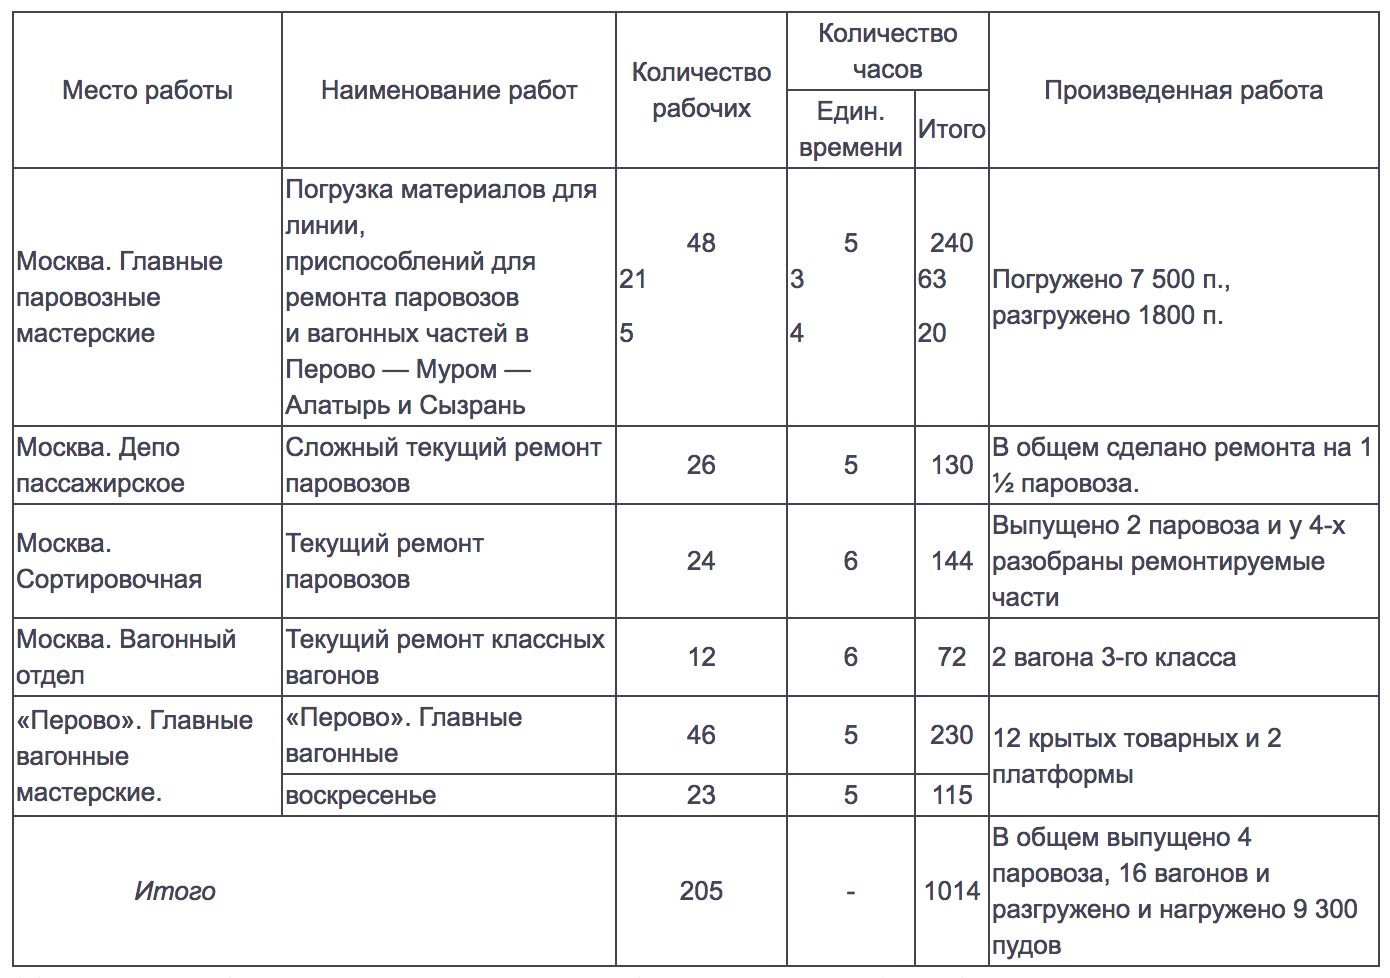
\includegraphics[width=10cm]{pictures/fig-1.png}
  \caption{Общая стоимость работы по нормальной оплате 5000 тыс. рублей, сверхурочной в 1 1/2 раза больше. Интенсивность труда по нагрузке выше обыкновенных рабочих на 270\%. Остальные работы приблизительно такой же интенсивности.}
  \label{fig:fig1}
\end{figure}

\begin{parnumbers}
Устранена задерживаемость заказов (срочных) по недостатку рабочей силы и волоките от семи дней до трех месяцев.

Работа происходила при наличии неисправности (легко устранимой) приспособлений, задерживавших отдельные группы от 30 до 40 минут.

Администрация, оставленная для руководства работами, едва успевала подготовить новые, и, может быть, немного преувеличено выражение старика-мастера, что в коммунистическую субботу сделано работы за неделю, против работы несознательных и расхлябанных рабочих.

Ввиду того, что на работах присутствовали и просто искренние сторонники Советской власти и ожидают наплыва таковых на будущие субботы, а также желания других районов взять пример с коммунистов-железнодорожников Московско-Казанской дороги, я остановлюсь подробнее на организационной стороне по сообщениям с мест.

На работах было процентов 10 коммунистов, постоянно работающих на местах. Остальные — занимающие ответственные посты и выборные, от комиссара дороги до комиссара отдельного предприятия, а также профессионального союза, и работающих в управлении и Комиссариате путей сообщения.

Воодушевление и дружность работы небывалая. Когда без ругани и споров рабочие, конторщики, управленцы, охватив сорокапудовый бандаж колеса для пассажирского паровоза, перекатывали его на место, как трудолюбивые муравьи, на сердце рождалось горячее чувство радости от коллективного труда и крепла вера в непоколебимость победы рабочего класса. Мировым хищникам не задушить победителей-рабочих, внутреннему саботажу не дождаться Колчака.

По окончании работ присутствующие были свидетелями невиданной картины: сотня коммунистов, уставших, но с радостным огоньком в глазах, приветствовала успех дела торжественными звуками Интернационала — и казалось, что эти победные волны победного гимна перельются за стены по рабочей Москве и, как волны от брошенного камня, разойдутся по рабочей России и раскачают уставших и расхлябанных.

Оценивая этот замечательнейший «пример, достойный подражания», «Правда» от 20 мая в статье тов. Н. Р. под этим заглавием писала:

«Случаи подобного рода работ коммунистов — не редкость. Я знаю о таких случаях на электрической станции и на различных железных дорогах. На Николаевской дороге коммунисты проработали несколько ночей сверхурочно, на подъемке свалившегося в круг паровоза; на Северной дороге, зимой, все коммунисты и сочувствующие проработали несколько воскресений, очищая пути от снега, ячейки многих товарных станций, в целях борьбы с хищениями грузов, совершают ночные обходы стан-ций, — но эта работа была случайной, не систематической. Товарищи казанцы внесли то новое, что делает эту работу систематической, постоянной. «До полной победы над Колчаком», постановили товарищи казанцы, и в этом все значение их работы. Они удлиняют на один час рабочий день коммунистов и сочувствующих на все время военного положения; одновременно они показывают пример продуктивной работы.

Этот пример уже вызвал и должен вызвать дальнейшие подражания. Общее собрание коммунистов и сочувствующих Александровской железной дороги, обсудив военное положение и постановление товарищей казанцев, постановило: 1) Ввести «субботники» для коммунистов и сочувствующих Александровской железной дороги. Первый субботник назначается 17 мая. 2) Организовать коммунистов и сочувствующих в примерные, показательные бригады, которые должны будут показать рабочим, как надо работать и что в действительности можно сделать при нынешних материалах, инструментах и питании.

По словам товарищей казанцев, их пример произвел большое впечатление, и на ближайшую субботу они ожидают на работы значительное количество беспартийных рабочих. Когда пишутся эти строки, в мастерских Александровской дороги сверхурочная работа коммунистов еще не началась, лишь слух о предполагающихся работах прошел, а уже беспартийная масса всколыхнулась, заговорила. «Мы не знали вчера, а то бы мы приготовились и тоже поработали», «в будущую субботу обязательно приду», — раздается со всех сторон. Впечатление, производимое такого рода работами, очень велико.

Примеру товарищей казанцев должны последовать все коммунистические ячейки тыла. Не только коммунистические ячейки Московского узла, — вся партийная организация России должна последовать этому примеру. И в деревнях коммунистические ячейки должны взяться в первую голову за обработку полей красноармейцев, помогая их семьям.

Товарищи казанцы закончили свою работу в первую коммунистическую субботу пением Интернационала. Если коммунистическая организация всей России последует этому примеру и будет неуклонно проводить его в жизнь, — ближайшие тяжелые месяцы будут пережиты Российской Советской республикой при громовых звуках Интернационала всех трудящихся республики...

За работу, товарищи коммунисты!».

«Правда» от 23 мая 1919г. сообщила, что

«17 мая на Александровской железной дороге состоялся первый коммунистический «субботник». 98 человек коммунистов и сочувствующих проработали, согласно постановлению общего собрания, 5 часов сверхурочно, бесплатно, лишь получив право вторично пообедать за деньги, причем к обеду за деньги же, как рабочим физического труда, было выдано по полфунта хлеба».

Несмотря на то, что работа была слабо подготовлена и слабо организована, все же производительность труда была выше обычной в 2 — 3 раза.

Вот примеры:

5 токарей в 4 часа сделали 80 валиков. Производительность по сравнению с обычной 213\%.

20 чернорабочих в 4 часа собрали старый материал в количестве 600 пудов и 70 вагонных рессор, по 3 1/2 пуда весом каждая, всего 850 пудов. Производительность по сравнению с обычной 300\%.

«Товарищи объясняют это тем, что в обычное время работа надоела, прискучила, а здесь работают с охотой, с воодушевлением. Но теперь стыдно будет в обычное время делать меньше, чем в коммунистический субботник».

«Теперь многие беспартийные рабочие заявляют о своем желании участвовать в субботниках. Паровозные бригады вызываются взять из «кладбища» паровоз в субботник, отремонтировать его и пустить в ход.

Получены сведения, что такие же субботники организуются на линии Вязьма».

О том, как идет работа в эти коммунистические субботники, пишет тов. А. Дьяченко в «Правде» от 7 июня. Приводим главную часть его статьи, озаглавленной «Заметки субботника»:

«С большой радостью собрался я с товарищем отбыть субботний «стаж» по решению железнодорожного подрайона партии и временно, на несколько часов, дать отдых голове, доставив работу мышцам... Нам предстоит работа на деревообделочном заводе дороги. Пришли, увидели своих, поздоровались, пошутили, сосчитали силу — всего 30... А перед нами лежит «чудовище» — паровой котел довольно солидного веса, пудов 600—700, и его-то и нужно нам «переставить», т. е. перекатить чуть ли не 1/4 или 1/3 версты к платформе. Сомнение закрадывается в наши мысли... Но вот мы уже стоим за делом: попросту товарищи подвели под котел деревянные катки, прикрепили две веревки, и работа началась... Подался котел неохотно, но все же пошел. Мы радуемся, нас ведь так мало... ведь этот самый котел тащили чуть ли не две недели рабочие-некоммунисты, числом втрое больше, а он упирался, пока не дождался нас... Работаем час, сильно, дружно под мерные звуки команды: «Раз, два, три» нашего тов. закоперщика, и котел идет да идет. Вдруг, что за оказия? Внезапно, смешно покатился целый ряд товарищей, — это «изменила» веревка в руках наших... Но минутная задержка: на месте ее укрепляем канат... Вечер, уже заметно темнеет, но нам нужно еще одолеть небольшую горку, и тогда работа будет скоро сделана. Трещат руки, горят ладони, нагреваемся, прем вовсю, — и дело спорится. Стоит «администрация» и, смущенная успехом, невольно тоже берется за канат: помогай! давно пора! Вот на нашу работу засмотрелся красноармеец. В руках его гармоника. Что он думает? Что за люди? Что им надо в субботу, когда все сидят по домам? Я разрешаю его догадки и говорю: «Товарищ! Сыграй нам веселую, мы ведь не какие-либо работнички, а настоящие коммунисты, — видишь, как у нас горит работа под руками, не ленимся, а прем». Красноармеец бережно кладет гармошку и скорей спешит к канату...

— «Англичанин мудрец!» — затягивает красивым тенором т. У. Мы вторим ему, и гулко раздаются слова рабочей песни: «Эй, дубинушка, ухнем, подернем, подернем...».

От непривычки мускулы устали, ломит плечи, спину, но... впереди свободный день — наш отдых, успеем выспаться. Цель близка, и после небольших колебаний наше «чудовище» уже почти у самой платформы: подкладывайте доски, ставьте на платформу, и пусть этот котел дает работу, которой уже давно ждут от него. А мы гурьбой идем в комнату, «клуб» местной ячейки, обвешанную плакатами, уставленную винтовками, ярко освещенную, и после хорошо спетого «Интернационала» лакомимся чаем с «ромом» и даже хлебом. Такое угощение, устроенное местными товарищами, как нельзя более кстати после нашей тяжелой работы. Братски прощаемся с товарищами и строимся в колонки-ряды. Песни революции оглашают в ночной тишине сонную улицу, мерные звуки шагов вторят песне. «Смело, товарищи, в ногу». «Вставай, проклятьем заклейменный» — несется наша песня Интернационала и труда.

Прошла неделя. Руки и плечи у нас отдохнули, и мы едем на «субботник» теперь уже за 9 верст, делать вагоны. Это — в Перово. Товарищи взобрались на крышу «американца» и звучно и красиво поют «Интернационал». Поездная публика прислушивается и, видимо, удивлена. Мерно стучат колеса, и мы, не успев влезть наверх, висим вокруг «американца» на лестницах, изображая «отчаянных» пассажиров. Вот и остановка, мы уже у цели, проходим длинный двор и встречаем радушного тов. комиссара Г.

— Работа есть, людей-то мало! Всего 30, а выпустить за 6 часов из среднего ремонта нужно чертову дюжину вагонов! Вот стоят размеченные скаты колес, есть не только пустые вагоны, еще и полная цистерна... но ничего, «приспособимся», товарищи!

Работа кипит. Я с пятью товарищами работаю важками, т. е. рычагами. Эти 60 и 70-пудовые колесные пары, под напором наших плеч, двумя важками, направляемые тов. «закоперщиком», живо и лихо перепрыгивают у нас с одних путей на другие. Одна пара убрана, — новая на ее месте. Вот уже всем им есть место, и мы это изношенное старье быстро-быстро по рельсам «сплавляем» в сарай... Раз, два, три, — подхвачены они на воздух железным вертящимся важком, и их уж нет на рельсах. Там, в темноте, идет стук молотков, то быстро, как пчелы, работают товарищи у своих «больных» вагонов. И столярят, и малярят, и крышу кроют, — работа кипит на радость нашу и тов. комиссара. А там понадобились наши руки и кузнецам. В переносном горне лежит раскаленное «правило», т. е. вагонный стержень с крюком, изогнутым неловким толчком. Белый, с искрами он очутился на чугунной плите и ловкими нашими ударами, под глазомером опытного товарища, принимает свою нормальную форму. Он еще бело-красный, а уже на плечах наших быстро-быстро подается к своему месту и с искрами вставлен в железную дыру, — несколько ударов, и он на месте. Лезем под вагон. Там устройство этих сцепок и правил совсем не так просто, как кажется, там целая система с заклепками и спиральной пружиной...

Кипит работа, темнеет ночь, ярче горят факелы. Скоро конец. Часть товарищей «приткнулась» у кучки ободьев и «потягивает» горячий чаек. Свежа майская ночь, и красив на небе серп молодого месяца. Шутки, смех, здоровый юмор.

— Товарищ Г., бросай работу, будет с тебя 13 вагонов!

Но тов. Г. этого мало.

Кончен чай, затянули свои победные песни, идем к выходу...».

Движение в пользу устройства «коммунистических субботников» не ограничивается Москвой. «Правда» от 6 июня сообщила:

«31 мая в Твери состоялся первый коммунистический субботник. На железной дороге работало 128 коммунистов. В 3 1/2 часа погружено и разгружено 14 вагонов, выпущено из ремонта 3 паровоза, распилено 10 саженей дров и произведены другие работы. Интенсивность работы квалифицированных рабочих-коммунистов превосходила обыкновенную производительность в 13 раз».

Затем в «Правде» от 8 июня читаем:

КОММУНИСТИЧЕСКИЕ СУББОТНИКИ

«Саратов, 5 июня. Железнодорожники-коммунисты, откликнувшись на призыв московских товарищей, на общем партийном собрании постановили: работать по субботам в течение пяти сверхурочных часов бесплатно для поддержания народного хозяйства».
\end{parnumbers}

\centering * * *

\begin{parnumbers}
  Я привел с наибольшей подробностью и полнотой сведения о коммунистических субботниках, ибо здесь, несомненно, мы наблюдаем одну из важнейших сторон коммунистического строительства, на которую наша печать обращает недостаточно внимания и которую мы все недостаточно еще оценили.

Поменьше политической трескотни, побольше внимания самым простым, но живым, из жизни взятым, жизнью проверенным фактам коммунистического строительства — этот лозунг надо неустанно повторять всем нам, нашим писателям, агитаторам, пропагандистам, организаторам и так далее.

Естественно и неизбежно, что первое время после пролетарской революции нас занимает более всего главная и основная задача, преодоление сопротивления буржуазии, победа над эксплуататорами, подавление их заговора (вроде «заговора рабовладельцев» о сдаче Питера, в каковом заговоре участвовали все от черной сотни и кадетов до меньшевиков и эсеров включительно1). Но рядом с этой задачей столь же неизбежно выдвигается — и чем дальше, тем больше — более существенная задача положительного коммунистического строительства, творчества новых экономических отношений, нового общества.

Диктатура пролетариата, — как мне приходилось уже не раз указывать, между прочим и в речи 12 марта на заседании Петроградского Совдепа, — не есть только насилие над эксплуататорами и даже не главным образом насилие. Экономической основой этого революционного насилия, залогом его жизненности и успеха является то, что пролетариат представляет и осуществляет более высокий тип общественной организации труда по сравнению с капитализмом. В этом суть. В этом источник силы и залог неизбежной полной победы коммунизма.

Крепостническая организация общественного труда держалась на дисциплине палки, при крайней темноте и забитости трудящихся, которых грабила и над которыми издевалась горстка помещиков. Капиталистическая организация общественного труда держалась на дисциплине голода, и громадная масса трудящихся, несмотря на весь прогресс буржуазной культуры и буржуазной демократии, оставалась в самых передовых, цивилизованных и демократических республиках темной и забитой массой наемных рабов или задавленных крестьян, которых грабила и над которыми издевалась горстка капиталистов. Коммунистическая организация общественного труда, к которой первым шагом является социализм, держится и чем дальше, тем больше будет держаться на свободной и сознательной дисциплине самих трудящихся, свергнувших иго как помещиков, так и капиталистов.

Эта новая дисциплина не с неба сваливается и не из добреньких пожеланий рождается, она вырастает из материальных условий крупного капиталистического производства, только из них. Без них она невозможна. А носителем этих материальных условий или проводником их является определенный исторический класс, созданный, организованный, сплоченный, обученный, просвещенный, закаленный крупным капитализмом. Этот класс — пролетариат.

Диктатура пролетариата, если перевести это латинское, научное, историко-философское выражение на более простой язык, означает вот что:

только определенный класс, именно городские и вообще фабрично-заводские, промышленные рабочие, в состоянии руководить всей массой трудящихся и эксплуатируемых в борьбе за свержение ига капитала, в ходе самого свержения, в борьбе за удержание и укрепление победы, в деле созидания нового, социалистического, общественного строя, во всей борьбе за полное уничтожение классов. (Заметим в скобках: научное различие между социализмом и коммунизмом только то, что первое слово означает первую ступень вырастающего из капитализма нового общества, второе слово — более высокую, дальнейшую ступень его.)

Ошибка «бернского», желтого, Интернационала состоит в том, что его вожди признают только на словах классовую борьбу и руководящую роль пролетариата, боясь додумывать до конца, боясь как раз того неизбежного вывода, который особенно страшен для буржуазии и абсолютно неприемлем для нее. Они боятся признать, что диктатура пролетариата есть тоже период классовой борьбы, которая неизбежна, пока не уничтожены классы, и которая меняет свои формы, становясь первое время после свержения капитала особенно ожесточенной и особенно своеобразной. Завоевав политическую власть, пролетариат не прекращает классовой борьбы, а продолжает ее — впредь до уничтожения классов — но, разумеется, в иной обстановке, в иной форме, иными средствами.

А что это значит «уничтожение классов»? Все, называющие себя социалистами, признают эту конечную цель социализма, но далеко не все вдумываются в ее значение. Классами называются большие группы людей, различающиеся по их месту в исторически определенной системе общественного производства, по их отношению (большей частью закрепленному и оформленному в законах) к средствам производства, по их роли в общественной организации труда, а следовательно, по способам получения и размерам той доли общественного богатства, которой они располагают. Классы, это такие группы людей, из которых одна может себе присваивать труд другой, благодаря различию их места в определенном укладе общественного хозяйства.

Ясно, что для полного уничтожения классов надо не только свергнуть эксплуататоров, помещиков и капиталистов, не только отменить их собственность, надо отменить еще и всякую частную собственность на средства производства, надо уничтожить как различие между городом и деревней, так и различие между людьми физического и людьми умственного труда. Это — дело очень долгое. Чтобы его совершить, нужен громадный шаг вперед в развитии производительных сил, надо преодолеть сопротивление (часто пассивное, которое особенно упорно и особенно трудно поддается преодолению) многочисленных остатков мелкого производства, надо преодолеть громадную силу привычки и косности, связанной с этими остатками.

Предполагать, что все «трудящиеся» одинаково способны на эту работу, было бы пустейшей фразой или иллюзией допотопного, домарксовского, социалиста. Ибо эта способность не дана сама собой, а вырастает исторически и вырастает только из материальных условий крупного капиталистического производства. Этой способностью обладает, в начале пути от капитализма к социализму, только пролетариат. Он в состоянии совершить лежащую на нем гигантскую задачу, во-первых, потому, что он самый сильный и самый передовой класс цивилизованных обществ; во-вторых, потому, что в наиболее развитых странах он составляет большинство населения; в-третьих, потому, что в отсталых капиталистических странах, вроде России, большинство населения принадлежит к полупролетариям, т. е. к людям, постоянно часть года проводившим по-пролетарски, постоянно снискивающим себе пропитание, в известной части, работой по найму в капиталистических предприятиях.

Кто пытается решать задачи перехода от капитализма к социализму, исходя из общих фраз о свободе, равенстве, демократии вообще, равенстве трудовой демократии и т. п. (как это делают Каутский, Мартов и другие герои бернского, желтого, Интернационала), те только обнаруживают этим свою природу мелких буржуа, филистеров, мещан, рабски плетущихся в идейном отношении за буржуазией. Правильное решение этой задачи может дать только конкретное изучение особых отношений между завоевавшим политическую власть особым классом, именно пролетариатом, и всей непролетарской, а также полупролетарской массой трудящегося населения, причем эти отношения складываются не в фантастически-гармоничной, «идеальной», обстановке, а в реальной обстановке бешеного и многообразного сопротивления со стороны буржуазии.

Громадное большинство населения в любой капиталистической стране, в том числе и в России, — а трудящегося населения и подавно — тысячи раз испытало на себе и на своих близких гнет капитала, грабеж с его стороны, всякого рода надругательство. Империалистская война, — т. е. убийство десяти миллионов людей для решения вопроса о том, английскому или германскому капиталу получить первенство в грабеже всего мира, — необычайно обострила, расширила, углубила эти испытания, заставила осознать их. Отсюда неиз-бежное сочувствие громадного большинства населения и особенно массы трудящихся к пролетариату за то, что он с геройской смелостью, с революционной беспощадностью свергает иго капитала, свергает эксплуататоров, подавляет их сопротивление, кровью своей пробивает дорогу к созданию нового общества, в котором не будет места эксплуататорам.

Как ни велики, как ни неизбежны мелкобуржуазные шатания и колебания назад, в сторону буржуазного «порядка», под «крылышко» буржуазии, со стороны непролетарских и полупролетарских масс трудящегося населения, тем не менее они все же не могут не признавать морально-политического авторитета за пролетариатом, который не только свергает эксплуататоров и подавляет их сопротивление, но который также строит новую, более высокую, общественную связь, общественную дисциплину: дисциплину сознательных и объединенных работников, не знающих над собой никакого ига и никакой власти, кроме власти их собственного объединения, их собственного, более сознательного, смелого, сплоченного, революционного, выдержанного, авангарда.

Чтобы победить, чтобы создать и упрочить социализм, пролетариат должен решить двоякую или двуединую задачу: во-первых, увлечь своим беззаветным героизмом революционной борьбы против капитала всю массу трудящихся и эксплуатируемых, увлечь ее, организовать ее, руководить ею для свержения буржуазии и полного подавления всякого с ее стороны сопротивления; во-вторых, повести за собой всю массу трудящихся и эксплуатируемых, а также все мелкобуржуазные слои, на путь нового хозяйственного строительства, на путь создания новой общественной связи, новой трудовой дисциплины, новой организации труда, соединяющей последнее слово науки и капиталистической техники с массовым объединением сознательных работников, творящих крупное социалистическое производство.

Эта вторая задача труднее первой, ибо она ни в коем случае не может быть решена героизмом отдельного порыва, а требует самого длительного, самого упорного, самого трудного героизма массовой и будничной работы. Но эта задача и более существенна, чем первая, ибо в последнем счете самым глубоким источником силы для побед над буржуазией и единственным залогом прочности и неотъемлемости этих побед может быть только новый, более высокий способ общественного производства, замена капиталистического и мелкобуржуазного производства крупным социалистическим производством.
\end{parnumbers}

\centering * * *

\begin{parnumbers}
  «Коммунистические субботники» именно потому имеют громадное историческое значение, что они показывают нам сознательный и добровольный почин рабочих в развитии производительности труда, в переходе к новой трудовой дисциплине, в творчестве социалистических условий хозяйства и жизни.

Один из немногих — вернее даже будет сказать: один из исключительно редких буржуазных демократов Германии, перешедших после уроков 1870—1871 гг. не к шовинизму и не к национал-либерализму, а к социализму, И. Якоби, сказал, что основание одного рабочего союза имеет большее историческое значение, чем битва под Садовой2. Это справедливо. Сражение под Садовой решало вопрос о первенстве одной из двух буржуазных монархий, австрийской или прусской, в деле создания национального германского капиталистического государства. Основание одного рабочего союза было маленьким шагом к всемирной победе пролетариата над буржуазией. Так и мы можем сказать, что первый коммунистический субботник, устроенный 10 мая 1919 года железнодорожными рабочими Московско-Казанской железной дороги в Москве, имеет большее историческое значение, чем любая победа Гинденбурга или Фоша и англичан в империалистской войне 1914—1918 годов. Победы империалистов есть бойня миллионов рабочих из-за прибылей англоамериканских и французских миллиардеров, есть зверство гибнущего, обожравшегося, заживо гниющего капитализма. Коммунистический субботник железно-дорожных рабочих Московско-Казанской дороги есть одна из ячеек нового, социалистического, общества, несущего всем народам земли избавление от ига капитала и от войн.

Господа буржуа и их прихвостни, включая меньшевиков и эсеров, которые привыкли считать себя представителями «общественного мнения», разумеется, издеваются над надеждами коммунистов, называют эти надежды «баобабом в горшке от резеды», смеются над ничтожным числом субботников по сравнению с массовыми случаями хищения, безделья, упадка производительности, порчи сырых материалов, порчи продуктов и т. п. Мы ответим этим господам: если бы буржуазная интеллигенция принесла свои знания на помощь трудящимся, а не русским и заграничным капиталистам ради восстановления их власти, то переворот шел бы быстрее и более мирно. Но это утопия, ибо вопрос решается борьбой классов, а большинство интеллигенции тянет к буржуазии. Не с помощью интеллигенции, а вопреки ее противодействию (по крайней мере, в большинстве случаев) пролетариат победит, устраняя неисправимо буржуазных интеллигентов, переделывая, перевоспитывая, подчиняя себе колеблющихся, постепенно завоевывая все большую часть их на свою сторону. Злорадство по поводу трудностей и неудач переворота, сеяние паники, пропаганда поворота вспять — все это орудия и приемы классовой борьбы буржуазной интеллигенции. Обмануть этим себя пролетариат не даст.

А если взять вопрос по существу, разве бывало в истории, чтобы новый способ производства привился сразу, без долгого ряда неудач, ошибок, рецидивов? Полвека после падения крепостного права, в русской деревне оставалось еще немало пережитков крепостничества. Полвека после отмены рабства негров в Америке, положение негров там сплошь да рядом оставалось еще полурабским. Буржуазная интеллигенция, в том числе меньшевики и эсеры, верны себе, служа капиталу и сохраняя насквозь лживую аргументацию: до революции пролетариата они упрекали нас в утопизме, а после нее они требуют от нас фантастически быстрого изживания следов прошлого!

Но мы не утописты и знаем истинную цену буржуазных «аргументов», знаем также, что следы старого в нравах известное время после переворота неизбежно будут преобладать над ростками нового. Когда новое только что родилось, старое всегда остается, в течение некоторого времени, сильнее его, это всегда бывает так и в природе и в общественной жизни. Издевательство над слабостью ростков нового, дешевенький интеллигентский скептицизм и тому подобное, все это, в сущности, приемы классовой борьбы буржуазии против пролетариата, защита капитализма против социализма. Мы должны тщательно изучать ростки нового, внимательнейшим образом относиться к ним, всячески помогать их росту и «ухаживать» за этими слабыми ростками. Неизбежно, что некоторые из них погибнут. Нельзя ручаться, что именно «коммунистические субботники» сыграют особо важную роль. Не в этом дело. Дело в поддержке всех и всяческих ростков нового, из которых жизнь отберет самые жизнеспособные. Если японский ученый, чтобы помочь людям победить сифилис, имел терпение испробовать 605 препаратов, пока он не выработал 606-ой, удовлетворяющий известным требованиям, препарат, то у тех, кто хочет решить задачу более трудную, победить капитализм, должно хватить настойчивости испробовать сотни и тысячи новых приемов, способов, средств борьбы для выработки наиболее пригодных из них.

«Коммунистические субботники» потому так важны, что начали их рабочие вовсе не поставленные в исключительно хорошие условия, а рабочие разных специальностей, в том числе и рабочие без специальности, чернорабочие, поставленные в обычные, т. е. самые тяжелые условия. Мы все хорошо знаем основное условие падения производительности труда, которое наблюдается не в одной России, а во всем свете: разорение и обнищание, озлобление и усталость, вызванные империалистской войной, болезни и недоедание. Последнее по важности занимает первое место. Голод — вот причина. А чтобы устранить голод, нужно повышение производительности труда и в земледелии, и в транспорте, и в промышленности. Получается, следовательно, какой-то порочный круг: чтобы поднять производительность труда, надо спастись от голода, а чтобы спастись от голода, надо поднять производительность труда.

Известно, что подобные противоречия разрешаются на практике прорывом этого порочного круга, переломом настроения масс, геройской инициативой отдельных групп, которая на фоне такого перелома играет нередко решающую роль. Московские чернорабочие и московские железнодорожники (конечно, имея в виду большинство, а не горстки спекулянтов, управленцев и т. п. белогвардейщины), это — трудящиеся, которые живут в условиях, отчаянно трудных. Недоедание постоянное, а теперь, перед новым урожаем, при общем ухудшении продовольственного положения, прямо голод. И вот эти голодные рабочие, окруженные злостной контрреволюционной агитацией буржуазии, меньшевиков и эсеров, устраивают «коммунистические субботники», работают сверхурочно без всякой платы и достигают громадного повышения производительности труда, несмотря на то, что они устали, измучены, истощены недоеданием. Разве это не величайший героизм? Разве это не начало поворота, имеющего всемирно-историческое значение?

Производительность труда, это, в последнем счете, самое важное, самое главное для победы нового общественного строя. Капитализм создал производительность труда, невиданную при крепостничестве. Капитализм может быть окончательно побежден и будет окончательно побежден тем, что социализм создает новую, гораздо более высокую производительность труда. Это — дело очень трудное и очень долгое, но оно начато, вот в чем самое главное. Если в голодной Москве летом 1919 года голодные рабочие, пережившие тяжелых четыре года империалистской войны, затем полтора года еще более тяжелой гражданской войны, смогли начать это великое дело, то каково будет развитие дальше, когда мы победим в гражданской войне и завоюем мир?

Коммунизм есть высшая, против капиталистической, производительность труда добровольных, сознательных, объединенных, использующих передовую технику, рабочих. Коммунистические субботники необыкновенно ценны, как фактическое начало коммунизма, а это громадная редкость, ибо мы находимся на такой ступени, когда «делаются лишь первые шаги к переходу от капитализма к коммунизму» (как сказано, совершенно справедливо, в нашей партийной программе3).

Коммунизм начинается там, где появляется самоотверженная, преодолевающая тяжелый труд, забота рядовых рабочих об увеличении производительности труда, об охране каждого пуда хлеба, угля, железа и других продуктов, достающихся не работающим лично и не их «ближним», а «дальним», т. е. всему обществу в целом, десяткам и сотням миллионов людей, объединенных сначала в одно социалистическое государство, потом в Союз Советских республик.

Карл Маркс в «Капитале» издевается над пышностью и велеречивостью буржуазно-демократической великой хартии вольностей и прав человека, над всем этим фразерством о свободе, равенстве, братстве вообще, которое ослепляет мещан и филистеров всех стран вплоть до нынешних подлых героев подлого бернского Интернационала. Маркс противопоставляет этим пышным декларациям прав простую, скромную, деловую, будничную постановку вопроса пролетариатом: государственное сокращение рабочего дня, вот один из типичных образчиков такой постановки4. Вся меткость и вся глубина замечания Маркса обнаруживается перед нами тем яснее, тем очевиднее, чем больше развертывается содержание пролетарской революции. «Формулы» настоящего коммунизма отличаются от пышного, ухищренного, торжественного фразерства Каутских, меньшевиков и эсеров с их милыми «братцами» из Берна именно тем, что они сводят все к условиям труда. Поменьше болтовни о «трудовой демократии», о «свободе, равенстве, братстве», о «народовластии» и тому подобном: сознательный рабочий и крестьянин наших дней в этих надутых фразах так же легко отличает жульничество буржуазного интеллигента, как иной житейски опытный человек, глядя на безукоризненно «гладкую» физиономию и внешность «блаародного чеаека», сразу и безошибочно определяет: «По всей вероятности, мошенник».

Поменьше пышных фраз, побольше простого, будничного, дела, заботы о пуде хлеба и пуде угля! Побольше заботы о том, чтобы эти необходимые голодному рабочему и оборванному, раздетому крестьянину пуд хлеба и пуд угля доставались не торгашескими сделками, не капиталистически, а сознательной, добровольной, беззаветно-героической работой простых тружеников, вот таких, как чернорабочие и железнодорожники Московско-Казанской железной дороги.

Мы должны все признать, что следы буржуазно-интеллигентского, фразистого подхода к вопросам революции обнаруживаются на каждом шагу повсюду, в том числе и в наших рядах. Наша печать, например, мало ведет войны с этими гнилыми остатками гнилого, буржуазно-демократического, прошлого, мало поддерживает простые, скромные, будничные, но живые ростки подлинного коммунизма.

Возьмите положение женщины. Ни одна демократическая партия в мире ни в одной из наиболее передовых буржуазных республик за десятки лет не сделала, в этом отношении, и сотой доли того, что мы сделали за первый же год нашей власти. Мы не оставили в подлинном смысле слова камня на камне из тех подлых законов о неравноправии женщины, о стеснениях развода, о гнусных формальностях, его обставляющих, о непризнании внебрачных детей, о розыске их отцов и т. п., — законов, остатки которых многочисленны во всех цивилизованных странах к позору буржуазии и капитализма. Мы имеем тысячу раз право гордиться тем, что мы сделали в этой области. Но чем чище очистили мы почву от хлама старых, буржуазных, законов и учреждений, тем яснее стало для нас, что это только очистка земли для постройки, но еще не самая постройка. Женщина продолжает оставаться домашней рабыней, несмотря на все освободительные законы, ибо ее давит, душит, отупляет, принижает мелкое домашнее хозяйство, приковывая ее к кухне и к детской, расхищая ее труд работою до дикости непроизводительною, мелочною, изнервливающею, отупляющею, забивающею. Настоящее освобождение женщины, настоящий коммунизм начнется только там и тогда, где и когда начнется массовая борьба (руководимая владеющим государственной властью пролетариатом) против этого мелкого домашнего хозяйства, или, вернее, массовая перестройка его в крупное социалистическое хозяйство.

Достаточно ли внимания уделяем мы на практике этому вопросу, который теоретически бесспорен для каждого коммуниста? Конечно, нет. Достаточно ли заботливо относимся мы к росткам коммунизма, уже теперь имеющимся в этой области? Еще раз, нет и нет. Общественные столовые, ясли, детские сады — вот образчики этих ростков, вот те простые, будничные, ничего пышного, велеречивого, торжественного не предполагающие средства, которые на деле способны освободить женщину, на деле способны уменьшить и уничтожить ее неравенство с мужчиной, по ее роли в общественном производстве и в общественной жизни. Эти средства не новы, они созданы (как и все вообще материальные предпосылки социализма) крупным капитализмом, но они оставались при нем, во-первых, редкостью, во-вторых, — что особенно важно — либо торгашескими предприятиями, со всеми худшими сторонами спекуляции, наживы, обмана, подделки, либо «акробатством буржуазной благотворительности», которую лучшие рабочие по справедливости ненавидели и презирали.

Нет сомнения, что у нас стало гораздо больше этих учреждений и что они начинают менять свой характер. Нет сомнения, что среди работниц и крестьянок имеется во много раз больше, чем нам известно, организаторских талантов, людей, обладающих уменьем наладить практическое дело, с участием большого числа работ-ников и еще большего числа потребителей, без того обилия фраз, суетни, свары, болтовни о планах, системах и т. п., чем «болеет» постоянно мнящая о себе непомерно много «интеллигенция» или скороспелые «коммунисты». Но мы не ухаживаем, как следует, за этими ростками нового.

Посмотрите на буржуазию. Как великолепно она умеет рекламировать то, что ей нужно! Как «образцовые», в глазах капиталистов, предприятия расхваливаются в миллионах экземпляров их газет, как из «образцовых» буржуазных учреждений создается предмет национальной гордости! Наша пресса не заботится, или почти совсем не заботится, о том, чтобы описывать наилучшие столовые или ясли, чтобы ежедневными настояниями добиваться превращения некоторых из них в образцовые, чтобы рекламировать их, описывать подробно, какая экономия человеческого труда, какие удобства для потребителей, какое сбережение продукта, какое освобождение женщины из-под домашнего рабства, какое улучшение санитарных условий достигается при образцовой коммунистической работе, может быть достигнуто, может быть распространено на все общество, на всех трудящихся.

Образцовое производство, образцовые коммунистические субботники, образцовая заботливость и добросовестность при добыче и распределении каждого пуда хлеба, образцовые столовые, образцовая чистота такого-то рабочего дома, такого-то квартала — все это должно составить вдесятеро больше, чем теперь, предмет внимания и заботы как нашей прессы, так и каждой рабочей и крестьянской организации. Все это — ростки коммунизма, и уход за этими ростками наша общая и первейшая обязанность. Как ни трудно наше продовольственное и производственное положение, все же за полтора года большевистской власти движение вперед по всему фронту несомненно: заготовки хлеба поднялись с 30 миллионов пудов (с 1.VIII.1917 по 1.VIII.1918) до 100 миллионов пудов (с 1.VIII.1918 по 1.V.1919); огородное хозяйство увеличено, недосев хлебов уменьшен, железнодорожный транспорт начал улучшаться, несмотря на гигантские трудности с топливом, и так далее. На этом общем фоне, и при поддержке пролетарской государственной власти, ростки коммунизма не зачахнут, а разрастутся и разовьются в полный коммунизм.
\end{parnumbers}

\centering * * *

\begin{parnumbers}
Надо хорошенько продумать значение «коммунистических субботников», чтобы извлечь из этого великого почина все громадной важности практические уроки, которые из них вытекают.

Всесторонняя поддержка этого почина — первый и главный урок. Слово «коммуна» у нас стало употребляться слишком легко. Всякое предприятие, заводимое коммунистами или при их участии, сплошь и рядом сразу уже объявляется «коммуной», — и при этом нередко забывается, что столь почетное название надо завоевать долгим и упорным трудом, завоевать доказанным практическим успехом в строительстве действительно коммунистическом.

Поэтому вполне правильно, по-моему, решение, созревшее у большинства ЦИК, отменить декрет Совнаркома в том, что касается названия «потребительских коммун»5. Пускай будет название попроще, — кстати, и недочеты, недостатки первых ступеней новой организаторской работы не будут взваливаться на «коммуны», а будут возлагаться (как это по справедливости и следует) на плохих коммунистов. Было бы очень полезно слово «коммуна» изгнать из ходячего употребления, запретить хватать это слово первому встречному, или признавать это наименование лишь за действительными коммунами, которые действительно доказали на практике (и единодушным признанием всего окрестного населения подтвердили) способность, уменье поставить дело коммунистически. Сначала докажи свою способность на бесплатную работу в интересах общества, в интересах всех трудящихся, способность «работать пореволюционному», способность повышать производительность труда, ставить дело образцово, а потом протягивай руку за почетным званием «коммуны»!

В этом отношении «коммунистические субботники» — самое ценное исключение. Ибо здесь чернорабочие и железнодорожные рабочие Московско-Казанской железной дороги сначала показали на деле, что они способны работать как коммунисты, а потом присвоили своему почину название «коммунистических субботников». Надо добиваться и добиться, чтобы это и впредь было так, чтобы все и каждый, кто называет свое предприятие, учреждение или дело коммуной, не доказывая тяжелым трудом и практическим успехом долгого труда, образцовой и действительно коммунистической постановкой дела, высмеивался беспощадно и предавался позору, как шарлатан или пустомеля.

Великий почин «коммунистических субботников» должен быть использован также в другом отношении, именно: для чистки партии. Совершенно неизбежно, что в первое время после переворота, когда особенно боязливо относилась масса «честных» и обывательски настроенных людей, когда буржуазная интеллигенция, включая, разумеется, меньшевиков и эсеров, поголовно саботировала, лакействуя перед буржуазией, совершенно неизбежно, что к партии правящей примазывались авантюристы и прочие вреднейшие элементы. Ни одной революции без этого не было и быть не может. Все дело в том, чтобы правящая партия, опирающаяся на здоровый и сильный передовой класс, умела производить чистку своих рядов.

В этом отношении мы начали работу давно. Надо продолжать ее неуклонно и неустанно. Мобилизация коммунистов на войну нам помогла: трусы и негодяи побежали прочь из партии. Скатертью дорога! Такое уменьшение числа членов партии есть громадное увеличение ее силы и веса. Надо продолжать чистку, используя почин «коммунистических субботников»: принимать в партию только после полугодового, скажем, «искуса» или «стажа», состоящего в «работе по-революционному». Такой же проверки потребовать от всех членов партии, вступивших позже 25 октября 1917 года и не доказавших особыми трудами или заслугами своей безусловной надежности, верности и способности быть коммунистами.

Чистка партии, связанная с неуклонным повышением ее требовательности насчет работы действительно коммунистической, будет улучшать аппарат государственной власти и гигантски приближать окончательный переход крестьян на сторону революционного пролетариата.

«Коммунистические субботники», между прочим, пролили необыкновенно яркий свет на классовый характер аппарата государственной власти при диктатуре пролетариата. Цека партии пишет письмо о «работе по-революционному»*. Мысль подана Центральным Комитетом партии в 100—200 тысяч членов (предполагаю, что столько останется после серьезной чистки, ибо теперь больше).

Мысль подхвачена профессионально-организованными рабочими. Их числится у нас, в России и на Украине, до 4-х миллионов человек. Они в гигантском большинстве за пролетарскую государственную власть, за диктатуру пролетариата. 200 000 и 4 000 000 — вот соотношение «зубчатых колес», если позволительно так выразиться. А дальше идут десятки миллионов крестьянства, которое распадается на три главные группы: самая многочисленная и самая близкая к пролетариату, полупролетарии или беднота; затем среднее крестьянство; наконец, весьма немногочисленная — кулаки или деревенская буржуазия.

Пока остается возможность торговать хлебом и спекулировать на голоде, крестьянин остается (и это неизбежно на известный период времени при диктатуре пролетариата) полутружеником, полуспекулянтом. Как спекулянт, он враждебен нам, враждебен пролетарскому государству, он склонен соглашаться с буржуазией и ее верными лакеями, вплоть до меньшевика Шера или эсера Б. Черненкова, стоящими за свободу торговли хлебом. Но как труженик, крестьянин — друг пролетарского государства, вернейший союзник рабочего в борьбе против помещика и против капиталиста. Как труженик, крестьянин своей громадной, многомиллионной массой поддерживает ту «машину» государства, которая возглавляется сотней-другой тысяч коммунистического пролетарского авангарда и состоит из миллионов организованных пролетариев.

Более демократического, в истинном смысле слова, более тесно связанного с трудящимися и эксплуатируемыми массами, государства на свете еще не бывало.

Именно такая пролетарская работа, которая знаменуется «коммунистическими субботниками» и проводится в жизнь ими, несет с собой окончательное укрепление уважения и любви к пролетарскому государству со стороны крестьянства. Такая работа — и только она — окончательно убеждает крестьянина в нашей правоте, в правоте коммунизма, делает крестьянина беззаветным нашим сторонником, а это значит: ведет к полному преодолению продовольственных трудностей, к полной победе коммунизма над капитализмом в вопросе о производстве и распределении хлеба, ведет к безусловному упрочению коммунизма.
\end{parnumbers}

28 июня 1919 г.

\end{document}